\documentclass[12pt,english]{report}

% % % These packages imported by Abe
\usepackage{xargs} 
%has to load before umlthesistemplate
\usepackage[colorinlistoftodos,prependcaption,textsize=tiny]{todonotes}
\newcommandx{\unsure}[2][1=]{\todo[linecolor=red,backgroundcolor=red!25,bordercolor=red,#1]{#2}}
\newcommandx{\change}[2][1=]{\todo[linecolor=blue,backgroundcolor=blue!25,bordercolor=blue,#1]{#2}}
\newcommandx{\info}[2][1=]{\todo[linecolor=OliveGreen,backgroundcolor=OliveGreen!25,bordercolor=OliveGreen,#1]{#2}}
\newcommandx{\improvement}[2][1=]{\todo[linecolor=purple,backgroundcolor=purple!25,bordercolor=purple,#1]{#2}}
\newcommandx{\thiswillnotshow}[2][1=]{\todo[disable,#1]{#2}}

%Has to load before umlthesistemplate
\usepackage{auto-pst-pdf}

%Can probably load anytime, but seems to work in advance...
\usepackage{graphviz}
\usepackage{microtype}
\usepackage{enumitem}
\usepackage{multicol}
\usepackage{caption}
\usepackage{subcaption}
\usepackage[toc,page]{appendix}
% From https://tex.stackexchange.com/questions/163330/creating-figures-to-show-binary-values
%For showing bitfields in the control hardware
\usepackage{bytefield}
\newcommand{\colorbitbox}[3]{%
\rlap{\bitbox{#2}{\color{#1}\rule{\width}{\height}}}%
\bitbox{#2}{#3}}
\definecolor{lightcyan}{rgb}{0.84,1,1}
\definecolor{lightgreen}{rgb}{0.64,1,0.71}
\definecolor{lightred}{rgb}{1,0.7,0.71}
% % % End Abe's stuff

\usepackage{umlthesistemplate}

\title{Command Language for Single-User, Multi-Robot Swarm Control}
\author{Abraham M. Shultz}
\pastdegrees{B.S. Worcester Polytechnic Institute (2004) \and M.S. University of Massachusetts Lowell (2014)}
\degree{Doctor of Philosophy}
\department{Computer Science}
\university{University of Massachusetts Lowell}
\majorprofessor{Dr. Holly A. Yanco}
\majorproftitle{Dissertation Chair}
\members{Dr. Radhika Nagpal \and Dr. Jay McCarthy}
\date{ 20 August, 2017}

\includeapproval
%Uncommenting any of these breaks the \begin{document} lines
\abstract{Command and control systems designed for a single operator to operate a single robot do not scale to control of swarms \citep{WangSearchScale}. User interfaces that require the user to attend to each robot overwhelm the controller when the number of robots increases beyond 12 or 13 for UAVs and 3-9 for UGVs \citep{WangSearchScale}. As robot swarms increase beyond these bounds, the control system must shift to controlling the swarm as a single entity. However, the form this interface should take to permit easy and understandable control of the swarm is largely undefined.

Previous work in HRI shows that multi-touch interfaces allow a scalable and direct mapping between the desires of the user and sequences of commands to robots \citep{micire2009multi}. By defining a mapping from user interface gestures to individual programs loaded on each robot, we can allow an individual to control arbitrarily large, heterogeneous swarms. This thesis presents an interface which extends previous work on multitouch interfaces for small groups of robots to larger swarms, and automates the process of converting command gestures into programs for each robot. The use of individual control programs rather than centralized control is important to realize the potential of swarms to continue to operate despite the possible failure of individual swarm robots.

The contributions of this thesis are a new swarm hardware platform, software to support it, and a user interface which converts user commands into programs for each robot in the swarm. The new swarm platform combines a wifi-enabled microcontroller with commodity mobility platforms sourced from children’s toys to allow large swarms to be built at a low cost. Because the design does not bind the implementation to a specific mobility platform, heterogeneous swarms can be constructed, using different toys. The hardware is also adaptable to new toys as older ones become unavailable, and could be used with custom-designed or 3-D printed mobility platforms. In order to maintain the low cost, sensors for the swarm robots are simulated with a top down camera. The use of simulation allows individual swarm members to be constructed cheaply in the present, while leaving the path clear in the future to push computation to the individual members as computer hardware becomes cheaper and smaller.
}

\acknowledgments{ Thank you to Dr. Holly Yanco, for encouraging me to turn one of my side projects into a dissertation, for providing guidance and resources for all these years, and finally for the encouragement to get out. Your ceaseless work to run the Robotics Lab and the NERVE Center and encourage a good mixture of freedom and focus for the people working there have made it a fantastic place to work. 

Thank you to Dr. Jay McCarthy for the useful pointers in programming languages and verification, and for keeping me on track when I was getting into the weeds of Turing completeness. 

Thank you to Dr. Radhika Nagpal for the loan of the E-Pucks, and for an impressive body of work in swarm robotics that inspired and informed some of this work. 

Thank you to Jonathan Roche for vastly speeding up the virtual laser, to James Kuczynski and Dalton Curtin for their attention to detail in coding the user responses, and everyone else in the UML robotics lab that I've asked to read papers, write ROS modules, or otherwise help out. Collaboration is one of our lab's strengths, keep it that way when I'm gone.  

Thank you to my parents, for teaching me, for encouraging me to pursue my own education, and putting up with the huge piles of messed-about-with hardware that follow me around. Your unconditional love and support has been a comfort to me in times of stress, and a joy always.

%Thank you to Vanessa Evers, Edwin Dertien, and the staff of the Human Media Interaction group at the University of Twente for hosting me while I worked on the swarm hardware. It was engaging and inspiring to ``do things with stuff'' with you. 
 }
\includetoc 
\maketitle

\begin{document}

\clearpage


\section{Intro/Research Statement}

Methods for command and control that are based on issuing individual orders to individual robots do not scale to large numbers of robots \cite{WangSearchScale}.
By defining a mapping from user interface gestures to individual programs loaded on each robot, we can allow an individual to control arbitrarily large, heterogeneous swarms.
Previous work in HRI shows that multi-touch interfaces allow a scalable and direct mapping between the desires of the user and sequences of commands to the swarm \cite{micire2009multi}. 
While swarm hardware is not yet at a point where very complex computation may be pushed directly to the swarm nodes themselves, that time is not far off. 
Until computational power in the individual swarm units does reach the levels required for complex computation, virtualization of computing resources can provide an adequate test environment for the development of swarm control algorithms at modest requirements in terms of space and power consumption. 
Centralizing the control of a large group of robots (a swarm) makes the system as a whole sensitive to the failure of the central controller. 
To avoid this type of failure, the overall action of the swarm should be guided by decentralized emergent behavior, rather than a centralized orchestration. 
Each robot receives its own program, and the sum of the execution of the programs on each robot results in completion of the task.
The various approaches to development of swarm robot control programs show that a wide variety of approaches can still result in robust controllers for swarm robots. 

\subsection{Problem Statement}

One potential method to control a swarm of robots is having a central computer dictate to individual robots how the robots should move.
However, centralized control is only as robust as the central controller. 
Distributed control systems do not have the single point of failure that centralized models have. 
In order to create reliable and useful swarm robotic systems, users must be able to specify a desired end state of the system that the swarm can converge to without reliable orchestration from a central controller. 
Moreover, this convergence must occur in the face of unreliability on the part of the individual swarm members. 

The current state of development of emergent control of swarms is guided by ad-hoc, iterative development models that are somewhat suited to software developers, but not suited to use by non-programming end users \cite{palmer2005behavioral}.
The motivating examples of uses for swarms are task oriented, such as sending swarm robots into disaster zones to search for survivors. 
While first responders are frequently trained in many specialized skills to perform their jobs, adding programming swarm robots to their training would be impractical. 
Even if first responders could be expected to develop software in a disaster zone, the situation frequently develops faster than the build/test cycles of software development can react. 
It is desirable to automate the construction of control software for a swarm so that it can adapt to a situation, without requiring significant development time. 
In order to support interactive control during a developing situation, the construction of the software should occur over a similar time scale to the user interactions.
Another possible example of an application for swarm robotics is cleaning, whether in a user's house, or in a more hazardous contaminated area. 

In either case, it is desirable for the user to be able to release the robots into the region with minimal oversight, and rely on the robots to discover what areas need cleaning, and to allocate robots to clean them. 
Modern household cleaning robots, such as the Roomba, are restricted to floors, and even specific types of flooring, but a heterogeneous cleaning swarm might include robots for cleaning windows and dusting surfaces as well. 
Currently, this kind of whole-house cleaning does not require programming the cleaning tools in advance, and any product which does require such a task is unlikely to succeed in the market. 

In order to remain useful in real-world applications, this work makes certain assumptions about the robots and the swarm. 
Networking between the robots is expected to be unreliable. 
Individual robots have limited transmission power over radio or infrared light links. 
Network links are also frequently attenuated by distance or intervening objects. 
As a result, when robots spread out into an area, some robots may not be directly reachable from others. 
Any software that purports to control a swarm under these conditions cannot rely on perfect connectivity for its operation. 

Robots' perception of their environment is frequently limited. 
Objects can block the sensing field of sensors.
Even without obstructions, most sensors have a limited effective range.
Because the real world is dynamic, robots can make only limited assumptions about what they cannot sense, and can only sense a limited area. 
Algorithms to control robots must primarily make use of locally sensed information, and secondarily make use of information received in communications from other robots. 

Because of the limited range of their sensing and networking, the localization of the robots may also be unreliable. 
GPS provides a global coordinate system in which robots can easily localize, but GPS signal is absent indoors, under dense tree cover, and in many other areas where it would be desirable to use swarm robots. 
The GPS signal is also weak, and so can easily be jammed by ambient RF interference or by malicious actors. 

Robots can also fail. 
The harsh conditions of the WTC rubble pile destroyed many of the robots sent in \cite{Micire02analysisof}.
In order to remain robust in the face of failures, algorithms should not be developed to depend on the perfect functioning of any individual robot. 
Rather, the behavior should emerge from the interaction of multiple, interchangeable robots, and tolerate the loss of individual robots up to some limit. 
In a situation where many or all of the robots attempting to complete a task are destroyed or disabled, it would be unreasonable to expect the task to be completed, but ideally, the bounds on how many robots are required to complete the task should be knowable. 

%A reliable robotic system is one that performs the required task, within some set of constraints, despite failures of some parts of the system. 
Cooperating systems can be broken down into two major classes, those that intentionally cooperate, and those that coopererate in the manner of ants or other swarm insects, without explicit agreements and planning \cite{parker1998alliance}.
The swarm-like approaches generally assume that the robots are homogeneous and all have the same control software. 
For the work described in this proposal, it may be that neither of these assumptions hold. 
The proposed hardware enables the creation of highly heterogeneous swarms, including variation in scale of the robots involved. 
Because the proposed control software generation scheme is intended to potentially result in different software for each robot, even robots with the same hardware may have different control programs. 
%However, the frameworks for analysis of explicitly cooperating multirobot systems may also not be applicable. 
%It is the intent of this project to have minimial explicit interrobot communication, which precludes many methods used to mutually plan tasks. 

%TODO: investigate CEBOT work 
%TODO: Is it possible to have the compiler compile to ALLIANCE specifications of task ability for each robot? Still has problems with sensing that task is done or other robots are doing it.
%TODO: ALLIANCE doesn't have an idea of minimum robots needed because even one robot can do the job, just more slowly. 
\subsection{Hypothesis}

There exists a number of robots beyond which users will transition from treating robots as individuals to interacting with the robots in small groups or as a single large group. 
This transition point will be apparent because of a change in the gesture set that the user uses to interact with the swarm. 
It is hypothesized that above the transition point, users will be more likely to neglect some subset of the available robots. 
The user will instead use commands that control the bulk of the robots as a cloud or flock, but may leave some robots unused. 
For example, the user may switch from selecting robots as individuals to shaping and pushing the swarm the way a child might play with a bug, putting their hand down so the bug goes around or avoids it, touching the back of the bug gently to make it scurry forwards, and so forth, or by shaping the group as if sculpting, with pushing and pinching to ``carry'' groups around. 
The user may also change how they indicate which robots are to be interacted with. 
Rather than selecting each robot by clicking on it, the may ``paint'' over the area containing the robots they want to use, or draw a circle around them. 
The size of the swarm where changes in the user gestures occur will indicate the transition point between the user intent to interact with individual robots as opposed to interacting with the swarm as a whole. 
%Harriet \emph{et al}. also put the estimated transition point between multi-agent control and swarm around 50 individuals \cite{harriott2014biologically}.  
%Above that threshold, human interaction may be able to remain focused on macro level behavior, influencing the overall behavior of the swarm rather than control of individuals.
%TODO is this relevant, if so, how?

Once the ratio of the size of individual swarm members to the size of the area the swarm is in becomes sufficiently large, displaying the swarm members at the same scale as the map will result in the representation of the swarm members being too small to interact with. 
This problem will arise at smaller scales if the swarm robots are themselves quite tiny, and some of the available swarm robots are indeed small \cite{pelrine2012diamagnetically}.
Scaling the representation of the robots up, relative to the map, will make the robot representations overlap unrealistically and obscure the map. 
Instead, we propose that for certain scales of swarms, it makes sense to represent the swarm as the area covered, rather than the locations of the individual robots.
This approach has been used successfully for navigation in three dimensions, by developing a controller that causes the individual UAVs to remain within a bounding prism, and allowing the user to control the shape and location of that prism \cite{ayanian2014controlling}.
Altering how the user interface displays the location of the robots in the swarm will affect the transition point. 
More specifically, a display which obscures individual robots and displays a cloud or swarm boundary will cause the user to treat the swarm as a whole rather than individuals, which will be apparent because the user will use different gestures. 

Further, it is hypothesized that it is feasible to convert user commands into programs for each robot which will converge to the desired behavior using only local sensing and local communications, and without resorting to global, absolute localization. 
However, this hypothesis must be modified with a few caveats. 
First, under the assumption that robots can fail, it is possible that the entire behavior can fail. 
For example, if enough of the robots are incapacitated, it may be that not enough are left to complete the task. 
It's also possible that at compile time, the task is still possible, but a later change of the environment renders it impossible. 
Assessing whether or not a user-specified action will be completed is not possible for all of the usual reasons that prevent prediction of the future, but in some limited cases, it may be possible to determine whether a specified action is impossible. The goal of this work is to provide a best-effort attempt to satisfy the user command, rather than prove anything about the possibility of doing so. 

%(Hadas http://link.springer.com/chapter/10.1007/978-3-642-22110-1_54#page-1 makes a distinction between unsatisfyable and unrealizable specifications. Unsatisfyable specs are those that the robot cannot do in any environment. Unrealizable specifications are those cases where there exist environments that can thwart the robot. In Hadas' work, there's also the idea that environments are finite in number. )
%\unsure{``Best effort", based on the information available, it's worth an attempt vs. not worth an attempt.}
%\unsure{So since we can't tell if a program will succeed, and determining if it is impossible might not be tractable, how do we know if we've written a compiler that does this?}



\chapter{Related Work}

Previous work in user interface gesture sets can be broadly separated into two classes: those that attempt to build a general gesture set, and those that attempt to build a gesture set to be used for a specific task. 

General gesture sets would be for operations such as the cut/copy/paste editing metaphors, which show up in word processing, image editing, and other productivity applications. 
These operations act in related but differing ways, depending on their context, but are invoked in the same way across applications and even across operating systems. 

Wobbrock, Morris, and Wilson use an interesting technique to elicit general user-interface gestures from non-technical users \citep{wobbrock2009user}.
The user is shown the \textit{effect} of a command, and then asked to perform the gesture that \textit{caused} that effect. 
The users were asked to think aloud, in order to understand their cognition about the system and gestures, in addition to their behaviour. 
The experiment used 27 commands: move a little, move a lot, select single, rotate, shrink, delete, enlarge, pan, close, zoom in, zoom out, select group, open, duplicate, previous, next, insert, maximize, paste, minimize, cut, accept, reject, access menu, help, task switch, and undo (listed in order of complexity as ranked by Wobbrock \textit{et al}).
Many of these commands are related to window managers, or occur in some form in multiple applications, such as the cut/copy/paste metaphors.

Task-specific gestures are for operations such as flying through a 3D rendering of an architectural space, or transposing cells in a spreadsheet. 
While somewhat intuitive gestures may exist for both operations, the operation is tightly bound to the task at hand, and the gestures would likely be different. 

Yao, Fernando, and Wang develop a set of task-specific gestures for urban planning from the required functionality of the interface and paper prototyping on a table \citep{yao2012multi}. 
The gestures were collected by placing a map on the table, and asking users to perform the gestures they would use to access the required functions. 
The resulting interface is modal, depending on the user's desired method of interaction, different gestures are available. 
The interface also permits the combination of some gestures, such as panning or rotating the map while zooming in or out at the same time. 

Micire \textit{et al}. develops a taxonomy of user gestures for control of both robots and of the interface to control them \citep{Micire:2009:ANG:1731903.1731912}. 
The interface control gestures are for actions such as zooming in on the content of the screen or panning around a map. 
Individual users chose a variety of gestures to perform the tasks, but for almost all types of tasks, having two gestures available to perform it would be sufficient to cover 60\% of the users. 
It was also noted that the gestures that users use are informed by their previous experience both with WIMP interfaces and with touch-screen technology. 
Since smartphones are a common multitouch interaction device, it would be expected that smartphone users expectations of multitouch interaction would be informed by their phones. 
Micire \textit{et al}. confirmed this, finding that iPhone owners used significantly more pinch gestures than participants with no iPhone experience. 
 
The more general gestures sets, such as those from Wobbrock, Morris, and Wilson, could be used in a gestural window manager or operating system interface. 
They are not tied to a specific application or working with a specific type or presentation of data.
The gesture sets developed by Micire \textit{et al}; Yao, Fernando, and Wang; or in this work are all intended to provide a more precise set of meanings for a single application and task. 

\section{Overview of Previous Swarm Hardware}

Swarm robots are generally small. 
The reason to keep swarm robots small is related to both the cost of making them and the cost of using them. 
Larger robots consume more materials per unit, and so cost more money.
As a result, for a given number of swarm units, larger robots will result in a higher cost swarm. 
Also, each robot requires some amount of space to move around in. 
To keep the ratio of free space to robots constant, the area of space used by the robots grows as the robots do. 
If the ratio isn't kept constant, the robots will crowd each other, and so large robots will require either a very large space, or become overly crowded.
Finally, larger robots are more cumbersome to deal with. 
They require larger storage areas, possibly teamwork to lift or repair, and so forth. 
All of these efforts are also multiplied by the number of robots in the swarm. 

The robots used in most swarm work are of a sufficiently small size that many of them can fit in a room. 
In addition to budgetary constraints, interaction with an environment built for humans places an upper bound the scale of the individual swarm members. 
For example, typical indoor doorways are around thirty inches wide, so a robot would have to be less than thirty inches wide to fit through them. 
The lower bound on swarm robots is generally dictated by fabrication technology, with smaller robots becoming increasingly difficult to assemble. 
As a result of these bounds, swarm robots are mostly between 1cm$^3$ and 0.3m$^3$. 
This scale range divides fairly evenly into robots that can operate in large swarms on a table, and those that can operate in swarms within a room, albeit possibly a large room. 
The challenge of construction of swarm robot hardware, then, is to put all of the same parts as non-swarm mobile robots: a mobility platform, a power supply, a processor, some sensors, and a communication system, into a small package.
Many impressive designs for small swarm robot platforms have been proposed and constructed as part of research in swarm robotics. 
However, most of these platforms are no longer easily commercially available, or never were. 

\subsection{Tabletop Swarms}

At the low end, in terms of size, the I-SWARM Project was intended to create a 2x2x1mm robot that moved by stick-slip locomotion actuated by piezo levers \citep{seyfried2005swarm}. 
Over the course of the project from 2004-2008, the hardware was developed and used in research, but was not converted to a commercial product.
Other techniques have been developed to use magnetic fields to apply force to small magnetic objects, resulting in controlled motion of the objects \citep{floyd2008untethered, pelrine2012diamagnetically}.
These systems are not amenable to decentralized control, because the moving components are not themselves robots. 
The moving parts are more accurately viewed as manipulators, with the instrumented environment, any sensors for feedback from that environment, and the manipulators themselves comprising a single robot. 

Alice, by Caprari \emph{et al}. \citep{caprari1998autonomous} combined a PIC16F84 processor, motors, RF and IR networking, and enough battery power for 10 hours of autonomy into a robot measuring under 2.5cm$^3$. 
The processor used in Alice is relatively underpowered compared to modern processors at the same price point and power consumption. 
Alice robots are no longer available for purchase. 


The Jasmine swarm robots were possibly the closest thing to a commercially-available successor to Alice  \citep{kernbach2011swarmrobot}.
Jasmine measured 26x26x20mm, and included an ATMega processor, IR close range communication and obstacle detection, two motor skid steering, and li-po batteries.
Unfortunately, Jasmine units cost about 100 Euro (\$111 USD) each when they were available, and they are no longer available for purchase. 
The plans and information required to reproduce Jasmine units are available for free at Swarmrobot.org.
Assembling a Jasmine robot is not beyond the reach of competent electronics hobbyists, but it does require some unusual build processes, such as grinding down the cases of certain electronic parts and filling holes in the PCB with solder to prevent light leaks. 
The chassis of Jasmine is also a custom mechanical assembly, rather than a commercially available product. 

InsBot was a small robot, measuring 41mm x 30mm x 19mm, that was designed to interact with cockroaches \citep{colot2004insbot}.
It used two processors, one to run higher level behaviors and one to interface with a suite of sensors that included 12 IR sensors and a linear camera. 
InsBots were never commercially available, and each required approximately 6 hours of work to assemble by hand. 
However, the construction process appears to have been relatively straightforward. 

The AmIR robot measured 6.5cm in diameter and 6cm tall. It has a more modern processor than Alice \citep{arvin2009development}.
There is no evidence that AmIR was ever widely available, and it cost \pounds65, or \$92 USD per unit \citep{arvin2015colias}.
The successsors to Amir, Colias and the related Colias-$\Phi$, are dual-microprocessor systems similar to Jasmine in functionality, but with additional features for pheremone robotics applications \citep{arvin2014colias, arvin2015colias}. 
It is built out of two PCBs, with the upper PCB and processor handling IR collision avoidance and communication, and the lower processor controlling the motors, power management, and a few other sensors.
Of particular note, the Colias-$\Phi$ lower processor is responsible for detecting light on the underside of the robot. 
Because of this downward facing light sensor, Colias-$\Phi$ robots can operate on an LCD screen or translucent table illuminated from beneath with a projector, for experiments in pheromone robotics. 
The light patterns displayed by the projector act as pheromones, which the robot can detect based on its position on the table. 
Colias robots cost \pounds25, or \$35US, in parts, but are not commercially available. 
The Colias-$\Phi$ model has an even more impressive price, at \pounds16, or \$22 USD.
Part of this drop in price may be due to the omission of the IR inter-robot communication system which Colias robots have. 

Even when they are commercially available, most existing swarm robots are too expensive to build a large swarm.
The E-puck from EFPL is approximately 800 Swiss francs (\$810 USD) per unit, so the cost of maintaining a large swarm can become daunting quickly. 
The high price of the E-puck is a result of its extensive suite of sensors, including a camera and 360$^{\circ}$ IR range sensor and communication system. 
E-pucks also require a fairly smooth operating surface.
The E-puck uses differential drive, and allows the front or back edge of the robot to serve as a skid. 
Due to the relatively sharp corner of the lower edges of the robot, the E-puck can become stuck on 2-3mm high obstacles. 

The r-one research robot is cheaper than the E-puck, at approximately \$220 USD per unit \citep{mclurkin2013low}. 
The developers of the r-one position it as a more-featureful and less expensive alternative to the E-puck (\$810, cannot sense neighbors without additional hardware), Parallax's Scribbler (\$198, minimal sensors), the iRobot Create (\$220, requires additional hardware to be programmable), the K-team Khepera III (\$2000), and the Pololu 3pi (\$99, minimal sensors). 
The main advantage in sensing that the r-one has over these other platforms is neighbor sensors and ground truth position sensing, both of which are implemented on the r-one using infrared.
The design of the r-one is open source, but it does not appear to be commercially available as of this writing.   

The Harvard Kilobots are a more recent entry to inexpensive swarms, and have been produced in large quantities \citep{rubenstein2014kilobot}. 
Kilobots contain about \$15 worth of parts, but a 10-pack sells for 1100 Swiss francs, or about \$112 (US) per robot. 
The Kilobots are intended for research in a highly homogeneous environment, with most or all of the robots executing the same program. 
As a result, they are designed to be programmed in parallel using an IR interface. 
For small groups, individual Kilobots can be programmed differently, but any attempt to give each of a very large collection of robots an unique program will take a long time. 
The Kilobots also move by stick-slip motion, and so must operate on a smooth surface, such as a whiteboard. 

One way to reduce the cost of swarm robots is to use commercial, off-the-shelf (COTS) hardware in the construction of the robot. 
Reusing existing hardware leverages the economies of scale that reduce the price of commercial hardware, as well as eliminating the need to design or build the COTS parts. 
Use of COTS parts in research robotics has led to at least two platforms referred to as COTSBots \citep{bergbreiter2003cotsbots, soule2011cotsbots}.
The first COTSBots used mote hardware for the communications link and sensing, plus a motor control add-on board \citep{bergbreiter2003cotsbots}. 
The mobility platform is a modified toy, in particular, a specific brand of high-quality micro RC car.
At the time of this writing, the car used in COTSBots is moderately expensive for a toy car, although quite cheap for a research robot, costing a little over \$100USD per unit. 
COTSBots use TinyOS, a modular and event-driven framework for developing node software \citep{levis2005tinyos}. 
TinyOS is written in a dialect of C called nesC. 
The motor and mote boards communicate using a messaging layer. 
The motor driver board is not commercially available, but can be custom-built by board fabrication companies, without the researcher having to assemble it by hand. 
The second COTSBots is larger, and will be discussed in the next section. 

\subsection{Room-sized Swarms}

One potential problem with extremely small swarms is that while the robots may scale down, the scale of obstacles they have to traverse may not scale with them. 
As previously mentioned, the Kilobots require a smooth surface, and the E-puck can be stopped by obstacles no more than a few millimetres tall. 
This sort of vulnerability prevents the smaller, tabletop swarm robots from operating well in human-scaled environments. 
In order to overcome this problem, larger swarm robots can be constructed.
 
The MarXbot swarm platform is capable of operating in unstructured human environments. 
MarXBots can also use their grippers to link themselves together and perform operations that an individual robot could not perform, such as bridging a gap larger than a single robot \citep{bonani2010marxbot}. 
The size and complexity of the MarXbots, as well as their powerful computer, renders the individual robots quite expensive. 

Swarmanoid extends the interlinking mechanism of MarXbot to a heterogeneous swarm with three different types of robots \citep{dorigo2013swarmanoid}.
The ``foot'' robots are MarXbots, and provide ground motion for ``hand'' robots. 
``Hand'' robots have grippers to manipulate objects, and can also climb.
The ``hand'' robots have an attachment point like the MarXbots, and so can be carried by ``foot'' robots. 
Flying ``eye'' robots provide overviews of the work area and networking.  

In order to reduce costs, another platform called COTSBots was developed \citep{soule2011cotsbots}.  
Instead of sensor motes on micro-scale RC cars, the newer COTSBots platform is composed of a laptop for processing and a modified RC car, tank, or similar toy as a mobility platform.
In order to interface between the laptop and motor drivers, a second micro-controller board, such as an Arduino or Phidget interface, may be used. 
Due to the diversity of possible combinations of hardware that can be assembled into this configuration, it is still a very viable platform. 
However, the minimum size of this style of COTSBot is the size of a laptop, which is in turn dictated largely by the minimum size of a useful keyboard. 
The large size of these COTSBots demands a very large space if the density of robots in a large swarm is to be kept low. 
Additionally, each laptop has a screen, keyboard, and so forth that are not useful while the robot is operating. 
All of these parts add to the overall cost of the swarm. 

Beyond the scale of rooms, swarm research has been done with Amigobots and Roombas, as well as larger custom platforms for outdoor multi-robot work \citep{guo2007bio, tammet2008rfid, olson2013cacm}.
In theory, swarm research could be performed using robots of any size, but financial limitations would place it out of the reach of most academic organizations. 

\section{UI Designs}

The user interface to a swarm has two functions. 
The first is to allow the user to provide input to the swarm, so that the user can direct the swarm to perform tasks. 
For the purposes of this research, the user interface is a multitouch surface that displays representations of the area the swarm is in and of the individual swarm robots \citep{micire2009multi}. 
The second function of a swarm user interface is to display information about the swarm, or to display information gathered by the swarm to the user. 
By providing an overview of the activities of the swarm, the user interface can give the user feedback on the progress of the task as it proceeds, as well as allowing the user to detect problems. 

Multitouch interfaces have been determined to improve on WIMP or voice interfaces for multi-robot control in a sequence of command and control tasks, including commanding the swarm to a location, performing reconnaissance, and having the swarm cross a dangerous area \citep{hayes2010multi}.
The interface displayed the locations of the robots on a directly manipulatable map, and used movable or semi-transparent user interface widgets, in order to minimize occlusion of the map. 
Areas were selected with with drawing gestures, and paths with fluid strokes, rather than e.g. selection of vertices bounding an area.
The use of multi-touch interaction is desirable because one-at-a-time selection doesn't scale beyond a very limited number of robots.
In order to interact with large groups of robots, the user must be able to perform operations on areas and groupings, rather than on the single point available with a traditional pointer-based interface. 

One approach to getting feedback from a swarm was the development of the Swarmish sound and light system \citep{mclurkin2006speaking}. 
Swarmish provides an ambient means of determining the overall state of the swarm, as well as some information about individual robots. 
The swarm that used Swarmish had autonomous charging, and so the individual robots had long runtimes, and minimal one-on-one interaction with humans. 
The ``ambient'' aspect of the interaction is that the information is continuously available, and the human user ``tunes in'' to it when needed. 
Swarmish uses a set of colored lights and sounds, produced by each robot, to provide feedback. 
The lights were in three colors, and had a total of 108 different combinations of colors and blink sequences, as a visual indicator of the state of each robot. 
In addition to the lights, each robot could produce MIDI notes over its audio system. 
Each note could vary in instrument, pitch, duration, and volume, as well as having tempos and rhythms as the code executes. 
The designers of Swarmish indicate that the sum of the audio output of the swarm could provide a overall idea of the status of the swarm, but that as a musical instrument, it is difficult to play well. 
Further, the use of lights as signaling mechanisms assumes that you can look at the robots. 

If we accept the assumption that the robots are visible to the user, the robots can carry some form of display that provides local information to the user. 
This information can then be displayed as an overlay in the real world, with the display of the information conterminous with its presence \citep{Daily:2003:WEI:820752.821587}. 
Local display of local information works if the user is part of a hybrid human/robot team, and so is in the same location as the users. 
However, there are many situations where the robot is not in the same location as the user. 
A common example is urban search and rescue, where buildings may be known to be unsafe, or of unknown stability, but it is desirable to search them for trapped people. 
In such a situation, the human user would rather be located elsewhere, and receive information from the robots. 

For situations where the user is not located in the same area as the robots, one possible approach is a ``call center'', where robots can request human attention when required \citep{chen2011supervisory}. 
The human in the call center, however, is faced with having to answer potentially multiple calls with no awareness of the robot's situation. 
The theoretical basis for call center UI is Supervisory Control. 
Supervisory control has the human act as the planner and monitor of the systems being supervised, but allowing the systems to operate on their own.
Automation is frequently broken down into ten levels of automation, with level 10 being a fully automatic system with no humans involved, and level 1 having no automation, such as a bicycle \citep{parasuraman2000model}. 

It would be expected that reducing the number of times the human is required to interact with the robot will permit the user to operate more robots.
With level one automation, the user has to interact constantly, and so could not be expected to operate more than one robot. 
By increasing the level of autonomy of the robot, the time required for the user to operate the robot decreases.
Instead of continuous interaction, the user can specify actions for the robot to undertake, and then ignore the robot while it performs the actions.
It is expected that the robot's effectiveness will decline over time since the last user interaction. 
This time that the robot operates without interaction before its effectiveness declines to a fixed minimum is called ``neglect time"\citep{olsen2003metrics}.
With increasing autonomy, neglect time increases.
The fifth level of the autonomy scale is operation by consent, where the computer chooses a route and executes it if the human permits it. 
The ninth level is the inverse of the fifth.
Rather than asking the user for consent to act, the robot acts autonomously and informs the human only in exceptional cases. . 
At the higher levels of the autonomy scale, the robot's neglect time far outweighs the time the user is expected to operate it, and so the user could reasonably be expected to operate other robots during the neglect time. 

Increasing neglect time may allow the user to operate more swarm robots, but it comes at a cost. 
The longer a user goes without learning about the state of one of the robots, the less idea they will have of the situation when they are called upon to operate that robot. 
The problem of automation decreasing the situational awareness (SA) of the user has been described in cockpit automation for aircraft \citep{wiener1980flight}, and generalized well to other systems that combine automation with human control \citep{kaber1997out}. 
If the user takes a long time to relearn the situation, the efficiency of the system will drop. 
Worse, the user may make errors because of an incorrect understanding of the system when they begin operations after a long neglect time \citep{cummings2008predicting}. 
One possible approach to maintain a constant and manageable workload on the user is adapting the level of automation to the workload. 
When the load is low, the user is more directly engaged, but when load is high, there is more automated assistance. 
By varying the level of automation, the workload for the user is kept constant. 
A constant workload is desirable because the user remains engaged with the work, and so has an ongoing understanding of the situation as it develops. 
The user is not suddenly called into a situation after remaining disengaged for some time. 
However, the workload must also be manageable. 
If the user is overloaded, their attention will become subject to triage, and they will begin to miss elements of the task. 
Adaptation does not have to be based on measured load, but could instead be based on perceived load or physiological markers in the user. 
%\citep{goodrich2010maximizing}

However, in situations with even moderate numbers of robots, even relatively high levels of automation may overwhelm the user \citep{lewis200617}. 
Level five, operation by consent, is a fairly high level of autonomy, but with a large number of robots checking in, even this level may generate too many events for the human to deal with. 
Increasing the autonomy to level nine, so that the robots are only checking in with the operator when an exceptional situation occurs, may still overwhelm the operator if enough robots are active.
Increasing the use of automation may also create new difficulties by leaving operator out of practice, or encouraging mis-placed trust in the automation's ability \citep{lee2004trust}. 

In fact, any kind of multitasking may prove insufficient for large swarms. 
For teleoperation, the best case is uncrewed aerial vehicles (UAVs), which require relatively little oversight. 
Uncrewed ground vehicles (UGVs) require more oversight than UAVs, due to the higher complexity of the ground environment. 
Estimates place the limits on the number of robots under control at 12 or 13 for UAVs and 3-9 for UGVs \citep{WangSearchScale}.  
There is some latitude, at least in UGVs, to increase multitasking by increasing automation, as shown by the relatively wide range in the interaction limits, but even 9 robots per operator is nowhere near the scale of kilo-robot swarms  \citep{Olsen:2004:FMH:985692.985722}.
Failure generally takes the form of task effectiveness no longer increasing as more robots are added.
Instead, the amount of time the user spends interacting with the robots begins to outweigh the neglect time, and so the robots spend increasing amounts of time waiting for interactions \citep{cummings2008predicting}. 

Ecological interface design (EID) presents a possible guide to the architecture of user interfaces for swarm robotics, and has been used in interfaces with mixed human-robot teams \citep{vicente1992ecological, gancet2010user}. 
In EID, a user's abilities that enable them to interact with a system is separated into a taxonomy of skills, rules, and knowledge. 
The user has skills, which are rote, simple activities that form the basis of the normal operation of the system. 
The user also knows a set of rules about the system. 
Rules allow the user to handle exceptions or unusual cases that have come up before. 
Rules do not require the user to understand the system, just to know that when certain situations are recognized, certain actions must be performed in response. 
Beyond rules and skills, the user also has knowledge of the system. 
Knowledge allows the user to handle novel exceptions. 
Knowledge gives the user an understanding of how the system works, and can apply that understanding to react to situations that the user has not experienced or been told about before. 
Events are also broken into three levels: routine, which uses skills; foreseen exceptions, which use rules; and unforeseen exceptions, which use knowledge. 
All levels should be supported by the interface, but the user should not be forced to operate at a higher level than is required. 
The abstraction of the process maps onto the hierarchy of ecological design, with the highest level being the function of the process and the lowest level being how the function is accomplished. 
At each level, there are constraints on the process that are used to define the normal operation of the process.
Detection of exceptions requires the display of all constraints, because exception is the breaking of constraints, and undisplayed constraints cannot be assessed to determine if they have been broken.

The user should be able to extract meaning from the information display quickly, as in the case of Swarmish and the robot-as-pixel UI designs.
By using the lights in Swarmish, the user can assess the state of individual robots, but by listening to the overall sound of the swarm, the user can also assess the behavior of the system as a whole.
The state and status lights of an individual robot is the low level in EID, watching how an individual action of the overall process is progressing. 
The ``tune'' of the entire swarm, produced by the sum of their MIDI notes, provides the high level overview, where a user can tell if the system is progressing well or developing problems. 
As the system changes, the changes and predictions should be highlighted so that the user understands consequences of their actions. 
In Swarmish, sudden changes in the tone or tempo of the swarm tune indicate transitions in its behavior, without the user having to observe the actions of the robots closely. 

EID is well-positioned to deal with emergent behavior, because the emergent behavior of the entire system is present at the functional level, but is composed of actions at the physical level.  
The control of swarm robots can be viewed as a hierarchy of increasing abstraction. 
At the least abstract, base level are the individual interactions of the swarm robots with each other and their environment, as dictated by their explicit programs. 
Above that level is the implicit, emergent behavior of the swarm as a whole. 
Finally, the most abstract level is the user intent, as expressed in the interface through their gestures. 
This hierarchy corresponds well to the abstraction of process in EID, with discrete physical actions at the lowest level and the overall results of the process at the highest level. 
Consequently, the user is permitted to issue commands in the most abstract domain, and the system can propagate them ``downwards'' into the concrete actions of the robots in the world, while also propagating information from individual robots ``upwards'' into the global view. 

Automation in EID allows the user to operate primarily with rules and knowledge, dealing with exceptions \citep{vicente2002ecological}.
The interface should allow direct manipulation of perceptual forms that map directly onto work-domain constraints and represent all of the information identified by the abstraction hierarchy. 
In a swarm context, this means displaying functional information in such a way that the user can move across the hierarchy from individual swarm bots to high-level swarm-wide tasks, and interact at all levels to control the swarm. 
More practically, this means that the information displayed must be integrated in such a way that the mapping from one unit of information to another is made apparent in the interface, rather than offloaded to the user to compute in their head \citep{yanco2004beyond}. 
For example, if a robot can send video and range information, the video and range information can be projected into a 3D space around the robot, rather than being displayed in separate UI windows.
Such a projection allows the user to easily relate visual and range information, and relate that information to the ongoing robot control task, which in turn increases task performance \citep{ricks2004ecological}.
Previous work in multi-touch interfaces directly satisfies these requirements of EID by providing both an omniscient camera view for direct manipulation of the high-level, functional actions of the entire swarm, and the ability to move down the hierarchy to control individual swarm members \citep{Micire:2009:ANG:1731903.1731912}.
The ability to display information about individual robots along side or on top of the interface representation of the robot is an important method of providing feedback to the user \citep{Kato:2009:MIC:1520340.1520500}. 

\subsection{Existing UI Designs}

Previous work in human-swarm interaction (HSI) shows an interesting diversity of methods to convey a command to a swarm. 
One approach, for co-located swarms, has the user making hand signals to the robots. 
If the swarm is equipped with cameras, the hand signs can be recognized visually by members of the swarm \citep{nagi2014online, giusti2012human, nagi2014human}. 
Because the recognition is performed by multiple robots at once, with different views, the robots can confer among themselves to arrive at a better understanding of the sign used.
Another approach to gesture control of swarms is to have the human and gesture recognition hardware separate from the swarm \citep{alonso2015gesture}.
This approach also allows the software to use the user's gestures to select part of the swarm by natural methods, such as pointing at robots. 

Another approach is the management of attractive and repulsive forces in the interface, which are conveyed to the robots. 
This style of interface maps reasonably directly to at least three of the programming paradigms used in swarm robotics. 
In physicomimetics, the attractors or repellents are points in the field that act on the robots through the same forces that the robots use in their interaction with each other. 
To cause robots to gather in an area, the user could place a source of virtual gravity there, which would draw robots towards it. 
In pheromone robotics, the effect would be much the same, but would be expressed as a pheromone source that diffused into the space and attracted robots. 
In vector fields, the vector field itself would be changed so that all vectors pointed towards the desired location. 

\citep{rusak2016affordances}
Affordances for designing natural user interfaces for 3D modelling
Zoltán Rusák, Ismail Cimen, Imre Horváth and Aadjan van der Helm
	Physical and anthropomorphic aspects of hand gestures
	Discussion of various matching methods
	Have to balance what can be detected by the technology with what the user finds appropriate
	Users asked to do gestures for various modeling actions
		motions, rotations of object
		Selection of object
		motion/rotation of camera/zoom
		extrude
		undo
		etc.
	Validation by doing the tasks
		Qualitative accuracy assessment
	Error types
		1 - hand motion isn't part of the UI, so system doesn't recognize it
		2 - system fails to recognize an action that is part of the UI
		3 - errors due to limitations of the tracking technology
	Mouse and keyboard took less time, but more actions
		It would be nice to know how an "action" is defined...
	Extrusion and delete tasks had most of the errors
		Mostly type 2 \& 3, so the gesture chosen by the designer was bad


Multitouch user interfaces don't generally have an agreed-upon standard for the gestures used in interaction with them, largely due to the relative novelty of the technology. 
The interface itself can be viewed as a message from the developer to the end user, which hopefully conveys enough information about the design of the interface to the end user that they are able to use it \citep{derboven2012semiotic}. 
The MuTable user interface in Derboven, De Roeck, and Verstraete uses a heirarchy of menus, which the user can explore and interact with. 
A multitouch user interface could attempt to do away with menus entirely, to encourage a direct interaction with the representations of the system objects on the screen, which would appear to reduce the interface to the point that there is not enough of it to convey a message. 
However, as long as the system both provides ways for the user to issue commands, and ways to return the results of those commands to the user, failures to figure out ways to issue commands and unwanted results are also a part of the interface that the user can interpret. 


	
\citep{musse1999guiding}		
Guiding and Interacting with Virtual Crowds in Real-Time
Soraia Raupp Musse, Fabien Garat and Daniel Thalmann
	Virtual crowds for simulated worlds
	Programmed, autonomous, or guided/interactive control
	UI allows people to type in messages to be sent to the crowds, text boxes and a big "SEND" button
	Guided crowd has some autonomy, can be told to go do specific actions or react to triggered events

\citep{mufti2017intguitive}
IntGUItive: Developing a Natural, Intuitive Graphical User Interface for Mobile Devices
Ammaar Amin Mufti
	Ha ha ha "Natural, Intuitive"
	Depth as a guide
		highlighting and shading
		static light in upper l of screen
		buttons on top of screen plane, screen controls below it
		non-interactive elements should stay flat/have no perspective
	Transition from skeuomorphism to flat/minimal
	Zooming-based UI


Early in the development of multitouch user interfaces, it became apparent that the window, icon, menu, and pointer (WIMP) interface would not be the best way to interact with novel interface technologies \citep{van1997post}. 
WIMP interfaces are tied to a metaphor of a desktop, where a user interacts with 2D spreadsheets and documents. 
To extend to information with higher dimensionality, the interfaces become more complex and less direct. 
The somewhat precient model proposed in by van Dam is a multi-modal interface of gestures and natural language, as is found in modern smartphones. 
This paper also shows an early example of a two-handed manipulation of a virtual object in a 3D environment, which presages the direct interaction style of multitouch user interfaces. 

The directness of user interactions as how much the interaction resembles the same interaction with physical objects, such as flipping pages of a calendar. 
With a physical calendar, one can turn pages by sliding a finger over them. 
Having a slider or buttons to switch months in a virtual calendar is thus less direct, and with a mulitouch interface, can be replaced by the same finger motion that would flip a page of a physical calendar. 

Keeping design elements of an object the same when the object is moved to a new material or created by new techniques is called ``skeueomorphism", and the copied design elements are ``skeueomorphs''. 
There are several reasons for skeueomorphs in design of user interactions. 
One reason is effectively kitsch. 
Design elements can be kept, despite not having a function in the new medium, simply because people find it entertaining to keep the appearance.
The vestigial jug handles on bottles of maple syrup or the yellow ``paper'' background of Apple Notes prior to its redesign are an example of this type of skueomorphism.
The jug handles are too small to use as handles, and the ``paper'' of Apple notes has no effect on the functioning of the application. 

Another reason to keep a design element, especially in multitouch UIs, is that the design element may provide hints to the user as to how the object can be interacted with. 
For example, in displaying photos, if the photo has a slight border, and the border appears to curve and ``lift'' off the screen background slightly, it will imply that the photo is a mobile object with a small space under it, and so could have other photos under or on top of it. 
If the photo is displayed totally flat, without a border, it will look more like a sticker or part of the background, and not imply that it can be moved. 
In neither case is the image actually ``above'' the background, but the visual impression to the user provides a clue for interacting with it. 

In the study of interactions with tangible interfaces, it has been proposed that the use of skueomorphic interfaces can also bridge between these two reasons for their use \citep{gross2014skeu}.
Rather than simple functionality, or pure amusement, the use of skueomorphic interface designs can convey messages about abstract qualities of a product to a user. 
One example given by Gross, Bardzell, and Bardzell is a digital synthesizer with a user interface that copies the knobs and switches of physical analog synthesizers. 
While this is likely not an optimal interface for controlling the synthesizer, it has connotations of quality, performance, and reference to more traditional electronic instruments, and so appeals to the user's idea of themselves as an artist and a participant in a tradition of artists. 

Intel has fielded drone fleets of up to 1,200 Shooting Star UAVs \citep{IntelDronesPage}. 
While the control system for the drones is proprietary, some information about the user interface can be gleaned from the promotional videos for the controller. 
The user interface for the creation of the light show appears to be very similar to those used in 3D rendering of computer graphics, including a timeline across the bottom of the screen, a preview in the center, and toolbars along the top and sides for interaction with the show. 
Visible tabs on the interface include "Curves/Surfaces", "Poly Modeling", "Sculpting", "Rigging", "Animation", "FX", "FX Caching", and "HEALTH". 
These different tabs are likely different ways to configure the shape of the formation in 3D (Curves, Poly Modeling, and Sculpting), animating the resulting formation (Rigging, Animation, and FX), and determining the state of the swarm as a whole (HEALTH). 

A screen that is likely part of the health interface is shown in one video \citep{OlympicTech}.
The screen has a grid of circles, colored various intensities of green, yellow, and red, as well as one shade of gray. 
The intensity may convey a different quality about the drone than the color, allowing at least two different dimensions of data per circle. 
As all the circles are displayed in a grid, an overview of the swarm health can be obtained by glancing at the display and assessing the relative balance of green vs. red. 

The user interface can import some form of data about the landscape where the drones will be launched, so the show can be positioned relative to hills or other obstacles in the area. 
The interface also supports at least some level of touch interaction, as users are shown pressing UI element buttons and rotating 3D renderings in the promotional videos. 

The interface for the drone light shows allows single users to fly hundreds to over a thousand drones, but it appears to be designed to create the show in advance, and execute it under central control. 
The drones themselves are well-localized, having GPS, barometers, and likely IMUs. 
The IMUs are likely based on Ascending Technologies AscTec Trinity autopilots, as Intel acquired AscTec in 2016. 

A number of systems propose pheromone-like control by the use of projected light in the area of the robots. 


One implementation of a human-swarm allows the human operator to describe the desired density of robots at locations within an operating area \citep{diaz2017human}. 
The use of density, rather than robot count, scales with the swarm size.
The desired configuration of the swarm can be drawn by the user on a tablet, and then converted to an update control law for the robots.
Alternatively, the user can directly place Gaussian functions in the space and vary their parameters. 
The resulting desired densities are smoothed to avoid discontinuities.
The use of density over location is similar to a number of interface methods that function by allowing the user to specify attractors and repulsion points in the swarm space \citep{goodrich2011toward, brown2014human, vasile2011integrating, kira2009exerting}. 

Goodrich et al use an attractor model under two different design metaphors, physicomimetics and a biomemetic model based on the dynamics of schooling fish, to solve an abstract information foraging problem \citep{goodrich2011toward}. 
The human influence is applied to a swarm system that is capable of some aspects of the problem without supervision, but is improved by the addition of human control. 
In keeping with the bio-inspired metaphor, the human can either control a leader, which the other members of the swarm are attracted to and follow, or a predator, which repels and can chase other members of the swarm. 
Leader-based models tend to lead to more stable, long-running interactions, as the members of the swarm move to remain near the leader, increasing the duration of the human operator's influence on the leader. 
In contrast, predator models result in high turnover of the swarm members that the human can influence, as the ``prey'' elements of the swarm act to get away from the predator's influence. 
This turnover is part of the two invariants proposed for swarm interaction by Brown et al, which are that the collective state is the fundemental perception of the swarm, rather than the individual robot, and that the ability of a person to influence and understand the collective state is determined by the balance between span and persistence \citep{brown2015two}. 
Persistence is the duration of each interaction with the swarm, and span is how many units the user interacts with. 
In a leader-based control UI, the span and persistence are both kept high, because the swarm elements are attracted towards the leader and remain under its influence for longer. 
In the predatory/repellent model, the span and persistence are low, because the other swarm elements flee from the user-controlled predatory unit. 

Brown, Kerman, and Goodrich demonstrate that a swarm can be controlled to form two different higher-level structures, a flock and a torus, by managing abstract attractors rather than individual behaviors. 
Further, the transition between modes was amenable to human control, so the overall behavior of the swarm could be configured with a relatively small set of tunable parameters. 
While the paper only indicates two possible modes, the torus and flock, these two behaviors are a relatively good match for the publicized behavior of the Perdix military drone swarm. 
Flock is a useful behavior for organized motion to a location, while the torus mode is good for loitering and overwatch of an area, matching the point-orbit, and move-to-point functions that are visible in videos of the Perdix UI. 
However, public materials on the Perdix system indicate that it uses a playbook interface, where the user selects from a set of available ``plays'', which the swarm then executes, rather than an explicit management of attractor parameters \citep{PerdixFactsheet}. 

Parasuraman, Galster, and Miller examined the use of playbook, waypoint, and combined playbook and waypoint control on robot teams in a capture-the-flag task \citep{parasuraman2005flexible}.
Playbook control provides a delegation layer to the interface, where the user does not have to specify the minutia of how a task is completed. 
The use of delegation decreases mission time and increases success, in this case, winning the game of capture-the-flag.
%If you have low span, you need long persistence to make a change
%Citation of mulitple fan-out papers
%Need to manage group, not individuals
%"Other work has estimated fan-out using large simulation studies involving several sizes of robot teams (Olsen \& Wood, 2004; Olsen, Wood, \& Turner, 2004)."
%"Pourmehr, Monajjemi, Vaughan, and Mori (2013) examine group-level abstracted multi-robot control to form dynamically-sized teams to increase fan-out."
%Interestingly, this tendency of an attractive/leading force to produce stronger and more persistent influences than a repulsive/pushing force is mirrored in natural integrative systems. If you attempt to blow or push a fluid, it succumbs to turbulence almost immediately, but drawing it with a continuous attractor results in coherent structures. The wind, for example, is generally a motion towards a low pressure zone, and streams are a motion downhill, but attempting to use pressure to push doesn't result in a coherent structure. Fuller's tensegrity stuff actually is based on this. 

There have been previous studies of the behavior of users in control of swarms with poor localization and bandwidth constraints \citep{nunnally2012human}. 
These constraints are realistic, as the motivating examples for swarm robotics, such as urban search and rescue or planetary exploration on e.g. Mars take place in locations where high-speed and high bandwidth networking infrastructure may be absent. 
The study describes a task similar to foraging, but under human control, where a 30-robot swarm is used to find a sequence of targets. 
The interface is mouse-based, and allows the user to issue two commands, "head towards the selected point" and "stop". 
The robots had gaussian error added their estimated location and orientation, meaning that the robots could start on a heading that was not exactly towards the selected point, when the user gave them a point to move towards. 
However, the robots had a consensus algorithm that would allow them to match heading with neighbors, which acts to counter the error in their initial headings. 
There were three conditions: low swarm-to-swarm bandwidth with low swarm-to-user bandwidth, high swarm-to-swarm with low swarm to user bandwidth, and high swarm-to-swarm bandwidth with high swarm-to user bandwidth.
The results showed that the medium bandwidth condition, with high swarm-to-swarm bandwidth but low swarm-to-user bandwidth was sufficient to complete the task. 
The users did adapt their behavior to match the information they had available, issuing more commands closer together in the medium bandwidth condition to drive the swarm into a smaller region and increase intra-swarm connectivity. 
In the low bandwidth condition, the user did not receive updates about the swarm condition often enough to enable them to maintain a dense swarm, and as a result, had trouble finding targets. 
The fact that the user interface and the user's intuition about the swarm could drive adoption of different behaviors supports the use of different rendering schemes for the swarm to encourage different user control strategies or conceptualizations about the swarm. 

Nunnally \emph{et al} explored the condition where a limited amount of information was available, but the time it takes for that information to become available (latency) is another factor in human-swarm interaction \citep{walker2012neglect}.
In the study , the latency was either absent, present both between members of the swarm and between the swarm and the user, and present, but the interface to the user predicted future swarm motion and displayed it. 
The task was similar to Nunnally \emph{et al}, in that the swarm was used to search a region for targets in a foraging task. 
The swarm could be commanded to move to a heading, stop, or flock under a model similar to boids \cite{reynolds1987flocks}.
The latency condition was significantly worse, in terms of targets found, than the no-latency condition, but the predictive display countered the latency sufficiently that the predictive and no-latency conditions were not significantly different. 
Interestingly, latency also drove the appearance of what the authors refer to as ``neglect benevolence", where the user not interacting with the system was not only tolerated, but actually helped improve the behavior of the system. 
Under latency, the user would issue a command, and then wait out the latency period to see how the system responded.
The resulting delay allowed operations such as flocking to converge and stabilize, thus increasing the swarm connectivity beyond what was attained in the no-latency condition. 

The previously discussed work on attractor management and control under latency and bandwidth restriction is concerned with UI design for swarm robots from the point of view of controllability and influence, which is to say whether or not the user can maintain desirable aspects of the swarm under the given conditions. 
It is not largely concerned with whether the interface itself, as presented in the experiment, is the best way for the user to attempt to control the swarm.
That is to say, the interface is taken as a fixed point, and the experimental condition is variation in the quality of the link between the user interface and the swarm. 

Humphrey et al assess the scalability of a multiple-robot control interface that uses a ``halo'' around the view from the currently-controlled robot to provide awareness of the positions of the other robots \citep{humphrey2007assessing}
The commands available to control each robot were high-level commands such as looking at specfic items or going to a point, which relied on the robot's autonomy, and more teleoperation oriented commands such as turning left or right, stopping, and moving. 
While this interface did appear to have a positive influence on the number of robots the user could control, it is not a swarm interface, but an interface for individual control of multiple robots. 

\citep{schoof2014bearing}
Bearing-Compass Formation Control: A Human-Swarm Interaction Perspective
Eric Schoof, Airlie Chapman, and Mehran Mesbahi
	Using only local information aids robustness: agent can act alone
	Version in this paper uses bearing only
	Also uses a compass to get rotation of robot in global frame
	Deals with predictability of the motion from an HRI view
		Example is preservation of scale and centroid when changing formation shape
	Control permits combination with human influence to allow scaling and translation of formation
	Very control-theoretic approach

\citep{kolling2013human}
Human-Swarm Interaction: An Experimental Study of Two Types of Interaction with Foraging Swarms
Andreas Kolling, Katia Sycara, Steven Nunnally, Michael Lewis
	"Currently, multi-robot approaches generally scale to at most ten’s of robots per operator even when using state of the art mapping, path planning, target detection, and coordination algorithms to alleviate the load on the operator (H. Wang et al., 2011; J. Wang \& Lewis, 2007)."
	2 kinds of interaction
		Intermittent
			User tells swarm when to change from one behavior to another
			Selection - active selection of robots
				Scales better to larger swarms
				Outperforms beacon
					Broader span and persistence
		Environmental
			User manipulates environment to cause swarm response
			Beacon - operates on robots within beacon range
	Paper also lists
		Persistent
			User provides a constant control input
				Predator/leader systems, single-joystick systems
		Parameter setting
			Attractor management
	UI appears to be very single-click mouse oriented




%\citep{tejada2003virtual}
%Virtual Synergy: A Human-Robot Interface for Urban Search and Rescue
%Sheila Tejada, Andrew Cristina, Priscilla Goodwyne, Eric Normand, Ryan O’Hara, and Shahrukh Tarapore
%	Robots build 3d VR map (Aibos + 2 blimps)
%	Virtual world acts as "memory" of the system, stores the things it has seen
%	System is based on Tekkotsu
%	Humans can interact with robots in VR
%	Student paper, probably undergrads
%	Not a lot of detail on UI evaluation

\subsection{The Interfaceless Interface}	

Some swarm robots are designed to be used with no control interface at all.
By altering the shape of simple stick-slip locomotion toys with laser-cut foam ``hats'' that change their outer perimeter, and changing the outline of the laser-cut foam forms they interact with, the random motion of the toys can create stable structures \citep{andreen2016emergent}).
The development of the shapes relies on human interaction, but specifying the shapes of the hats and interactive components seems amenable to solution with genetic algorithms. 
Because the toys used in this work were about \$4-8 USD, and everything else was composed of laser-cut foam, the platform is extremely inexpensive. 

\citep{gancet2010user}
User Interfaces for Human Robot Interactions with a Swarm of Robots in Support to Firefighters
Jeremi Gancet, Elvina Motard, Amir Naghsh, Chris Roast, Miguel Munoz Arancon and Lino Marques
	"Sahin [2] describes the swarm robotics as a (i) a large number, of (ii) homogeneous, (iii) autonomous, (iv) relatively incapable or inefficient robots with (v) local sensing and communication capabilities" - Could be the other Sahin definition I was looking for
	Remote v. Prximate interaction
	Early deployment to gather knowledge vs. synchronous deployemnt as helpers
	Details reasons firefighting is hard and how they constrain the interface design
	Light array visor
		LEDs on inside of visor as a HUD
		...I guess that's a good idea? Looks like it could be blinding.
	Paper cites EID, but I'm not sure the LAV is properly EID based on my understanding of it
	Paper mostly about LAV and data on tests with it
		Remote HSI evaluation was inerview with 4 firefighters
		Swarm seems to have been very small (4 robots?) and not very swarm-like
%The possibility of robots being designed so that their behavior is controlled by their physical form points towards a possible convergence of the physical design of swarm robots and physicomimetic swarm controls with design of macromolecules. 
%Rather than implementing physicomimetic controls in software, the resulting system would use the existing laws of physics as an element of its control program.
%These systems would construct structures larger than themselves as a consequence of how they react, chemically and physically, with their environment. 
%Each assembly step would be done by a vast number of robots so cheap and so fast to build that it is easier to synthesize new ones for each construction step than to build a general-purpose reprogrammable assembler. 


\subsection{Video Game UI Design}

\todo{Mobile video game design similar to top-down interaction with the 3M Multitouch monitor.}

\todo{Mark's work on video games, RTS gamers want menus}

Games with a similar top-down interface for control of multiple units generally appear in the genres of Real Time Strategy (RTS) games, Turn-based strategy games, and Multiplayer Online Battle Arena (MOBA). 

Realtime strategy games generally have the player playing against multiple other players, some or all of which may be controlled by the computer. 
The goal of the game is typically to acquire some form of resources, which are used to develop military units or units which accelerate the acquisition of further resources. 
The military units are then used to attack the other players, with the goal of the game being to be the only remaining player. 

Turn-based strategy games are similar to RTSs, but instead of all players acting simultaneously, each players actions are taken on their turn. 

MOBAs have a smaller focus and more rapid play than RTS or turn-based strategy games. 
Typically, there are multiple players, but each player is on one of two sides battling over some set of objectives on the world map. 
Rather than controlling multiple units, each player controls a single, powerful unit, and may be able to influence weaker, semi-autonomous computer-controlled units.  There may be resources as in RTS games, but typically they are far more limited in number.   

MOBAs, RTSs, and turn-based strategy games all have a similar user interface. 
The ``world'' or area of play is depicted as a map, typically viewed either top-down or an axonometric perspective. 
The map is where the main action of the game takes place, and displays the relative position of the characters and other elements of the game. 
Around the map are typically displays and interactive elements such as menus or buttons to interact with the game. 

The control of units in the game is typically done using the mouse to select units and send commands via mouse clicks, while one hand operates keys, typically on the left side of the keyboard, for other functions. 
How the keyboard is mapped depends on the pace of gameplay. 
For extremely rapid games, such as Defense of the Ancients (DoTA, a MOBA), there are a small number of key commands that can all be operated without removing the fingers of the left hand from the keyboard. 
DotA in particular uses mouse clicking, combined with the control, shift, and alt keys in various combinations, to perform all of the actions of gameplay \todo{cite https://dota2.gamepedia.com/Controls}. 

Age of Empires is a RTS. 
It is less fast-paced than DotA, but still takes place in realtime. 
Most of the keys of the keyboard are mapped to various commands, such as locating and selecting different types of units or buildings, or commanding those units and buildings. 
Commands to buildings typically cause the construction of various units, while consuming resources. 
For example, pressing `D' would find a Dock, and then pressing `A' would command the Dock to start work on a Fishing boat \todo{cite http://ageofempiresonline.wikia.com/wiki/List\_of\_Hotkeys }. 

Europa Universalis 4 uses the entire top row of letters on the keyboard to switch between different map modes, and every other key to activate some feature of the game, as well as mouse controls for interactions with individual units and locations \todo{cite https://eu4.paradoxwikis.com/Controls}. 
Europa Universalis gameplay does not take place in realtime, and the player may speed or slow the game clock, as well as pausing the game. 

Another common feature of MOBA, RTS, and turn-based strategy games is the ``fog of war". 
The entire map is normally hidden from the player until they command their units to enter an area, whereupon the area is revealed. 
In gameplay, the intent of fog of war is to prevent players from knowing about the opposing player's location without sending sorties. 
This lack of information is almost identical to that experienced by a teleoperator of a robot exploring an area with a SLAM algorithm, as the map is revealed to the operator as the robot moves into the area. 

\todo{graphic here to depict typical game UI}

% Previous work with top-down multitouch user interfaces has found that users who play video games express a desire for more UI ``widget'' interactions, that is, interacting with buttons, menus, or specialized user interface components \cite{Micire:2009:ANG:1731903.1731912}. 
Gamers who play RTS games also used fewer pinch gestures in a multitouch context, possibly because RTS games are typically played with a mouse and keyboard, which does not have a pinch-like gesture. 

% % TODO: Maybe use some of this stuff, but I don't have a good idea where
% %Emergent behaviors arise from the interactions of actors with each other and the world around them. 
%In the face of uncertainty in the world, the behaviors will also become uncertain. \change{cite trust work}
% %Programs synthesized to guide the swarm should be designed to be robust against failure or degradation of swarm members. 
% %The heterogeneity of the swarm may also be leveraged to increase its robustness against failures of individual nodes or alterations of the environment. 
% %However, because heterogeneity increases the dimensionality of the solution space for program synthesis, it may adversely affect the performance of the program synthesis and the swarm's runtime convergence to the desired state.
% %
% %A concept of the swarm as a whole as a programmable entity runs into trouble with reliability. 
% %In conventional compilation, assuming the compiler is correct and the computer is correct, the compiled binary does what the source code says. 
% %Robots interact with the real world, which is much less likely to be ``correct'' in the same sense a compiler can be asserted to be. 
% %Programs for swarms are only going to be functional within some probabilistic grounds and assumed conditions. 
% %This requirement indicates that the situation has to be at least somewhat known ahead of time, so that the robots will all receive programs that allow them to perform the task.
% %In the ideal case, the emergent action of all of the robots interacting with the environment causes them to perform the task. 
% %
% %Swarms have more uncertainty, because the reliability of individual robots is low; and higher attentional demands because there are many robots. 
% %It may be that above some threshold, the attentional demand will drop again, as the group is no longer treated as a large number of individuals, but as a single group. 
% %%A lot of Dr. Adams' work in HSI was under ONR Award N00014-12-1-0987
% %
% %If the user is unconcerned with the functioning of individual swarm members, so long as the swarm as a whole remains functional, the UI may simply drop malfunctioning individuals from view. 
% %This handling of error conditions on individual swarm units fits with the assumption that the swarm as a whole achieves robustness through redundant expendable units, while also allowing the human user to have a rough idea of how the situation is developing by watching the cloud shrink. 
% %Do long as progress appears to be being made on the mission, the user might let underperforming units slide. 
% %The supervisory system might not even announce when units are lost, until it starts to affect performance.  
 

\section{Swarm Software Development Methods}

Because the conversion of the specification of desired behavior for the swarm into individual programs for the swarm member robots is still an open question, it is necessary to understand the current methods used in the development of programs for swarm robots. 
Much of swarm robotic development follows the usual model of software development. 
Starting from a desired functionality, the developer writes a program that they think will provide that functionality.
The program is then tested, in simulation or on real robots, and its behavior is observed. 
The programmer then modifies their program to account for any observed difference between the desired function and the system's behavior. 
This loop of coding, testing, and coding again is repeated until the system behaves as expected, or the programmer graduates \citep{cham2010graduate}. 

Because the normal software development model is time-consuming, and outside of the abilities of many people who might want to use swarm robots, it is desirable to automate the development of software controllers for robots. 
One approach to the conversion of the command language to programs for the robots is to define a transformation from the command language to executable code. 
The transformation operation can be codified as a sort of ``compiler'', or more accurately, a code generator, which creates programs for the robots. 
The possibility of coding for the swarm as an entire system, rather than writing each robot's program independently, has given rise to several programming paradigms and domain-specific languages for robotic swarms. 

Another possibility is the composition of preexisting behaviors that each satisfy part of the user's desired behavior. 
Given some library of primitives, the user could select a sequence of behaviors, or conditions for the execution of behaviors, to build a complete program. 
Pheromone robotics provides one possible method of controlling this composition dynamically.
 
Still another approach is to allow the user to specify a desired behavior and evolving controllers to match it. 
It would be hoped that evolving the controllers would reduce the complexity of the development task to the definition of a suitable means of determining the fitness of the resulting program. 
Unfortunately, even this reduction does not permit an escape from iterative development. 

\subsection{Amorphous Computing}

Amorphous computing (AC), also called spatial computing, is computation using locally-linked and interacting, asynchronous, unreliable computing elements dispersed on a surface or throughout a volume \citep{abelson2000amorphous}. 
The motivation for AC is that while it may be possible to produce arbitrary quantities of ``smart dust'', it is not possible to ensure that it all works well and is precisely located, especially in real-world applications.
The goal of AC is to get useful work out of such materials, despite uncertainty as to their reliability and location. 
Smart dusts are also the limit case, in terms of scale, for swarm robotics. 
Indeed, most of the volume of existing swarm robots is motors and batteries, with the computational components taking far less space. 
If AC promises to get useful work out of smart dust, then it also has some applicability to larger swarm robots.

There are several languages intended to program amorphous computers. 
``Proto" is a language for a continuous plane spatial computer \citep{correll2009ad}.
Because the devices are distributed over a plane, the difficulty in communicating between any two devices is a function of the distance between them, much as with RF or other radiative communications.
In Proto, the behavior of regions of space is described by the programmer, and the description is transformed into local actions for the network of devices. 
Because devices have a size in the real world, and space between them, the devices cannot not have a one-to-one mapping with the space, but instead perform an approximation of the desired behavior. 
Swarm robots are mobile, so some swarm algorithms can be implemented as a description of constraints on the robot's state, such as ``the robot must have communications links to no more than 2 and no less than 1 other robots", and a command to move randomly unless the constraint is satisfied. 
Within a bounded environment, such an algorithm can be shown to converge to satisfy its constraints \citep{correll2009ad}. 

Proto also has considerable appeal as a programming language for swarm control development because of the layering in its structure. 
Proto is designed to map from behavior of regions at the global level to programs for discrete points at the level of individual devices \citep{beal2006infrastructure}. 
If user interface interactions can be interpreted as indications of desired behaviors displayed over spatial regions, then conversion of those behaviors into programs in Proto may be amenable to automation. 
Proto's layered structure also has a clear relationship to the hierarchical structure of EID, with the programming language serving as a user interface at the highest abstraction level of the interface design, but providing a smooth transition to the lower abstraction levels.  

Origami Shape Language (OSL) uses the abstraction of a foldable sheet to form shapes, inspired by both origami and the folding of epithelial cells during the development of biological organisms \citep{nagpal2004engineering, nagpal2001programmable}.
Regions and edges on the sheet can be defined by propagation of morphogens, and folds along the edges result in the development of the final form.
Because of the use of morphogens and local communication between the agents on the sheet, there is no need for a global controller to dictate the development of the final form. 
Further, because the high-level description of the desired form does not involve abstractions of the underlying modules, OSL could operate on interlocking modular robots, actuated flexible materials, swarms, or other kinds of computational media. 
In fact, the flexible sheet could be assumed to be virtual, and the resulting motions of the sheet could be translated into motor commands to configure swarm robots into specific arrangements in space. 

Growing Point Language (GPL) allows the specification of topological patterns in an amorphous computer, and so can also be used to specify the distribution of swarm robots, or behaviors of the swarm robots, in a space \citep{nagpal2004engineering}. 
GPL is inspired by the morphogenic controls present in biological organisms, which use gradients of chemicals called morphogens to dictate the development of cells \citep{turing1952chemical}.
The name GPL arises from one of the language's main abstractions, the growing point. 
The growing point is the location of activity within the amorphous medium, at which local agents are changing their state. 
Growing points move through the medium, affecting the state of the computational points they pass, and emitting pheromones into the medium which control the motion of growing points.

Importantly, GPL does not make any prior assumptions on the location of the particles in the system, or robots in the swarm, aside from that they are sufficiently dense in the medium. 
For swarm robotics, this is an important quality, as precise localization may not be available. 
Initially, all agents have the same state and program, with a few exceptions that serve as seeds for the growth to begin. 
If the pattern is not required to be fixed at a particular location, even the seeds could be undetermined initially, and elect themselves via a method such as lateral inhibition. 
During the execution of the GPL program, each agent chooses its state based on the presence of pheromones, which are morphogens with limited range. 
Range limitation on morphogens propagating between robots is set using a TTL (Time To Live) counter that propagates with the morphogen, and is decremented with each hop in the communication network. 
When the TTL hits zero, the morphogen message is no longer propagated. 
By controlling the production or propagation of morphogens within the amorphous medium, complex patterns can be developed. 

\subsection{Pheromone Approaches}

The abstractions of GPL bear a very strong relation to pheromone robotics. 
Pheromone robotics is a metaphor used in developing control software for swarm robots. 
Some social animals, especially insects, use chemical signals called pheromones to communicate with each other. 
For example, wasps inside their nest react to the scent of wasp venom by travelling to the outer surface of the nest and attacking nearby moving targets  \citep{jeanne1981alarm}.
Ants leave trails of pheromones for other ants to follow to food sources. 
Each individual ant's contribution to the trail can be modulated by the quality of the food source, which allows the reaction of the other ants to the trail to cause an emergent distribution of the foraging work force that favors higher-quality food sources \citep{sumpter2003nonlinearity}.
Because pheromones are chemicals with spatial locations, it would be possible to combine the use of pheromones with reaction diffusion equations to structure activity within a space or to converge to patterns of activity over time  \citep{turing1952chemical}. 
Assuming even diffusion of the robots in space, the global map of the pheromone concentrations is represented over the network by the locally-computed concentrations computed by each robot.

In pheromone robotics, the pheromones are usually simulated or ``virtual'' pheromones, rather than real chemicals which are detected by chemical sensors (for an exception, see \citep{hayes2001swarm}). 
Each pheromone can have properties such as diffusion and evaporation rates that result in the pheromone spreading in space or gradually disappearing. 
In addition to its properties, the pheromones may have other characteristics which robots can sense. 
For example, a robot may emit a pheromone which diffuses into the environment and evaporates quickly, so distance from the robot can be determined by the strength of the pheromone, and approaching or avoiding the robot may be accomplished by moving up or down the gradient of pheromone strength. 
If the swarm is engaged in a search, each searching robot may emit a ``search marker'' pheromone that lingers in the area after the robot leaves. 
Other robots, on entering the area, would detect the pheromone and know that searching this area again would be fruitless. 
If the object of the search can move, the marker pheromone could diminish as a function of time, so areas that have not been searched for a long time become unmarked and may be searched again. 
Once the target is found, the robot may stop and emit a ``discovery pheromone'', which diffuses into the environment, attracts other robots, and causes them to also emit a discovery pheromone. 
As a result, once any robot discovers the target, all of the robots quickly converge on its location. 

The addition of directional communication for the messages that convey virtual pheromone information allows easy determination of the direction of pheromone gradients \citep{payton2001pheromone}.
Rather than directly diffusing in the space as a chemical would, hop counts in the network of robots simulate diffusion. 
Because routes may be of different length, the message with the lowest hop count is assumed to be the truest indication of minimal distance within the network. 
Rather than modelling the world based on the incoming messages, the content of the pheromone messages and the network behavior as a whole serves as a model of the world, mapped 1:1 onto the real environment. 
While it is possible to build a set of behavioral primitives out of pheromone signaling and associated behaviors, controlling the swarm to perform a task with these primitives is still done by hand \citep{payton2003compound}.

In all of these examples, the sensing of the pheromones is assumed to be local to the robot, at least metaphorically. 
To actually maintain pheromones in the environment without robots being present to transmit them requires, again, a global representation of the task space which the robots can refer to when needed. 
Use of pheromones to guide swarm robots for simulated search and patrol tasks has been demonstrated, with the assumption that there is a central controller maintaining the concentration of pheromones on the map, and informing the swarm members \citep{coppin2012controlling}. 
In a real implementation, some robots could remain stationary and only act as transponders, computing and transmitting the local pheromone information for a given area. 
Another possible approach to enable pheromones in space is to operate the robots in an area which is illuminated by a projector. 
The projector can then color the area with light that the robots can sense, and modulate the intensity of the light to indicate the intensity of the pheromone \citep{arvin2015cosvarphi,diaz2017human}. 
However, even if the robots are limited to only the pheromones they can directly perceive and emit at the present instant, some emergent behaviors are still possible. 


It has been demonstrated that a swarm can perform construction tasks using only local sensing and no communication \citep{wawerla2002collective, bowyer2000automated}.
However, the addition of communication between systems and memory of the state of the world will improve the efficiency of the system.
The system under discussion was developed to have the task implied by the behaviors available for the agents, rather than generating the program from a higher-level specification, such as the form of the structure to be built.

Pheromone approaches can guide the construction of objects, even if the individual swarm members have no memory and only local perception \citep{mason2003programming}. 
The agents engaged in the construction move at random, and take actions governed by their individual perception of environment at present time. 
The agents can release and react to pheromones in the environment, and so there is an implicit communication via stigmurgy, but no explicit agent-to-agent communication. 
The set of rules that govern the mapping of sensor precepts to actions must be such that no point in the construction of the building can be mistaken for another, as that could result in loops or skipping parts of the building sequence. 
The TERMES project created a compiler that translates desired final structures into rules to guide the construction of those structures by cooperating agents \citep{werfel2014designing}.

Both global vector fields and the global and local blending of vector fields in co-fields can be viewed as subsets of pheromone robotics that use a global spatial representation. 
One approach to a control UI for a remotely-located swarm is a multi-touch interface for specifying a vector field \citep{Kato:2009:MIC:1520340.1520500}.
Because the user interface design focuses on the vector field rather than individual robots, the same control interface can scale to an arbitrarily large collection of robots. 
Vector field paths can have loops, which do not exist in waypoint-based paths. 
Waypoint paths have explicit ends, unless an additional command is added to join beginning and ending points. 

Vector field paths have substantial limitations. 
Because the vectors are bound to a 2-D plane, the paths they create cannot cross each other. 
Instead, they flow together. 
A 2-D vector field is also not a useful metaphor for controlling UAVs.
The vector field could be possibly extended into three dimensions, to control UAVs as well as ground vehicles, but there would have to be some form of discontinuity in the field to prevent assignment of UAVs to ground vehicle paths and vice versa. 
The vector field can be viewed as an abstraction of pheromone control, or even implemented in terms of the presence or absence of virtual pheromones, but it has some limitations that pure pheromone control does not have.
For instance, pheromones permit the presence of multiple pheromones at one point, with multiple meanings, but the vector field has one value for each point. 
Attempting to solve this problem by proposing multiple fields raises the question of how to combine them, and if a universal combination function applies at all points in the field, it raises the question of why they were not combined already. 

The vector field is also not very intuitive to users. 
Kato \emph{et al}. indicates that in order to use the vector field well, the users had to anticipate and project the future motions of the robots. 
Interface changes, such as showing particles on the vector field, could improve usability, but these approaches would have the same scaling problems that the robot representation does. 
When the view is zoomed out very far, individual whirls and eddies in the field may not be visible to the user. 

This vector field interface does not directly map to programs on the robots. 
Instead, the central computer maintains the vector field representation and commands the individual robots.
Vector fields also do not allow the assignment of tasks to robots, but allows the user to directly control the motion of the robots. 
In order to convert from a task-based user interface to a vector field representation, the task would have to be converted into a series of changes to the field.
Since the robots may not have accurate localization within the task space, it may not be possible to guide the robots by relating their position to a global vector field. 

The use of co-fields may provide a way to move the vector field representation from the central computer to the swarm, or allow the swarm to act for some time without constant updates from a central controller \citep{mamei2003co}.
Co-fields distribute the data within a space, which may be physical or may be abstract. 
Agents react to gradients in field, and spread their own fields over local communication networks. 
The overall vector space created by the user (the UI vector space) could be propagated to the robots periodically, and combined with their own internal vector fields to generate movement based on both the user's desires and the local rules operating on each robot. 
As with general vector fields, knowing which areas of the UI vector space are relevant to each robot may require global localization, and so only be available for swarms operating in conditions that permit global localization. 

\subsection{Compositional Approaches}

Rather than developing a novel control program for each robot automatically, it may be possible to compose programs from behavioral primitives, such that some combination of the primitives results in the emergence of the desired behavior. 
A compositional approach to program generation requires the definition of primitives out of which programs can be composed, and some degree of assurance that these primitives can cover the space of possible tasks required from the robot. 
One possible list of primitives is disperse (no other nodes within distance d), general disperse (no more than n nodes within distance d), clump/cluster, attract to location, swarm in a direction, and scan area \citep{evans2000programming}.
Another proposed catalog of behaviors for swarm control bases the simple behaviors on pheromones or chemical sensing in single cells \citep{nagpal2004catalog}. 
The proposed behaviors are the use of gradient sensing for position and direction information, local inhibition and competition, lateral inhibition for spatial information, local monitoring, quorum sensing for timing and counting, checkpoint and consensus sensing, and random exploration. 
The first five are common in amorphous computing as well, but the last three are not. %TODO what are their uses?. 
While these behaviors are themselves expressed in terms of pheromones, the composition of the primitives into complete programs is not dictated by a pheromone-based system.
Furthermore, compostional approaches have been proposed in control-theoretic terms as well as pheremone-based terms, so the process of composition of primitives can be viewed as a metastrategy for the creation of programs, rather than a process specific to pheremone robotics \citep{belta2007symbolic}.

The pheromone based approaches to swarm programming are sufficient for relatively complex behaviors. 
Quorum sensing is used to detect whether the local agent count is sufficient for a task. 
By detecting the presence of sufficient robots to perform a task, the robots can allocate themselves to tasks in a just-in-time manner, rather than being pre-allocated when the task is designed. 
Decentralizing the selection of robots, in turn, may be more robust against failures of individual robots, as it uses the robots that are in the right place at the right time, rather than waiting for specially assigned robots. 
However, under sufficiently bad conditions, a sufficient quorum may never arrive, deadlocking the task. 
In combination with domino timing, where completion of each phase triggers the next, locking at any step could then deadlock the entire process unless another mechanism detects and corrects it.

Individual robots can cooperate without communication to push an object to a beacon based on simple behaviors \citep{chen2015occlusion}. 
Each robot has two simple behaviors.
If the view of the beacon is blocked, and the robot is next to an object, the robot pushes on the object.
If the robots can see the beacon, it wanders and avoids obstacles. 
The sum of the two behaviors results in a net pushing force on the side of the object opposite the beacon, which moves the object to the beacon. 
There do exist certain pathological shapes which the system cannot move towards the beacon, but it is demonstrated to work for all convex shapes. 

Another compositional method for programming robots proposes that the behaviors can be separated into classes, such as motion, orientation, and so forth \citep{mclurkin2004stupid}. 
Among these behaviors are ``primitives'' such as several forms of clustering, which other, later works have treated as an emergent behavior itself, arising from more primitive primitives. 
The variable granularity of the primitives available to compose swarm control programs seems to point to a hierarchy of control elements, with perhaps single motor operations at the bottom, and an increasing composition of elements to create more and more complex behaviors.
Swarm control programs would then call multiple primitive behaviors, providing them with parameters such as degrees of bearing and centimeters of proximity. 
The behaviors ideally run concurrently, and some of them respond to sensor inputs. 
The output of behaviors is whether they are running, translational and rotational velocity for the robot, and LED configuration. 
Because multiple behaviors might specify differing outputs, subsumption and summation are used to arbitrate between behaviors of differing priorities. 

These emergent approaches do not have the robots perform all of their available actions all of the time. 
Instead, it is assumed that the behavior of each robot is controlled by its reaction to the environment around it, and possibly to signals from other robots, so that actions are only performed when they are required. 
As a result, user programs compiled from a higher-level representation could be a table consisting of possible values for the sensors, and the actions to undertake when those values are met.
Guarded Command Programming with Rates (GCPR) provides a formal framework for the analysis of this type of compositional program \citep{napp2011compositional}. 
Robots are assumed to only have local sensing.
The guards of GCPR are conditions on the environment.
When a condition is met, the robot performs actions at a given rate. 
In the concurrent case, this is modeled as each action happening one at a time, but in random order. 
On a real swarm, the actions would take place in parallel, but the concurrent model is more amenable to analysis. 
To determine if a set of actions will be successful, it is required to ensure that for all orderings of all actions, the final state space of the swarm is the desired final state. 
Correct programs are those that reach the target state with probability one, even when composed with bounded failures. 
Once the target state is reached, the program is assumed to halt, so while the final state may be reached very slowly, once it is reached, it is not left. 
In the GCPR models, the time to execution of an action is stochastic, but in the real-world case of noisy or imperfect sensors, the variable time to execution of a guarded behavior would be caused by the imperfection of the robot's ability to detect that the guard was satisfied. 

\subsection{Evolutionary Composition}

Determining how the behaviors should be composed for an individual swarm robot's controller is difficult. 
Unfortunately, much of the process of composing of programs for swarm robots consists of iterating between composing sets of primitives and observing behavior of the system in an ad hoc process, just as with the creation of control programs by coding \citep{palmer2005behavioral}. 
Rather than removing iterative software design from the process, it has simply been moved up one layer of abstraction, from writing code for the robots to composing that code from behavior primitives. 

One possibility is to permit composition to behave like the programming environment Tierra \citep{ray1991approach}.
In Tierra, there is no such thing as an invalid program. 
All sequences of the existent symbols are regarded as executable programs, although some are more useful than others. 
The possibility that programs can be ranked by some function creates the possibility that genetic algorithms (GA) can direct the automated composition of behavioral primitives into programs \citep{palmer2005emergence}.
A GA expresses the robot program as a genome, which is translated into the actual program and run on the robot. 
The result of running each program is assessed using a fitness function and then the genomes for the best programs are combined to produce a new generation of genomes. 
This cycle of combining and assessing genomes continues until a certain level of quality is reached, as judged by the fitness function.

Unfortunately, given the time required to iterate over multiple generations of controllers, genetic approaches are unlikely to be fast enough for interactive control of robots by a human user. 
However, it is still useful to examine the possibility of developing a fitness function as a way of investigating methods for automatically assessing the behavior of a swarm.
Without some way of determining the ``goodness'' of a swarm's behavior, it is useless to say that one algorithm or design paradigm is better or worse than another. 

In order to determine the quality of the behavior of the swarm, its behavior must be measured.
Harriott \emph{et al}. propose that metrics for measuring the interaction of humans and swarms differs significantly from the interaction of humans and individual robots, and can be broken down into 9 classes \citep{harriott2014biologically}. 
\begin{itemize}[noitemsep]
\item Human attributes - Interaction, trust, intervention frequency 
\item Task performance - Ability to accomplish task, speed, accuracy, cost
\item Timing - Command diffusion lag, behavior convergence
\item Status - Battery life, number of functioning members, stragglers
\item Leadership - Interaction between special members of the swarm and others
\item Decisions - Action selection, likelihood that the correct action is chosen
\item Communication - Speed, range, network efficiency
\item Micromovements - Relative motion of individual swarm elements
\item Macromovement - Overall swarm motion, flocking, elongation, shape 
\end{itemize}

Task performance is an especially interesting metric, but it is difficult to automatically extract from the observed behavior of the system an overall understanding of the progress it is making on the task, and so a value for the output of the fitness function. 
Worse, without a time bound on solving a problem or a way to calculate progress, it is impossible to tell if a program has failed, or has merely not yet succeeded.
For example, assume a program's intended purpose is to gather all of the units of a resource at a goal. 
If the program merely moves the units stochastically, sometimes they will enter the goal, creating an appearance of progress. 
However, it may be vanishingly unlikely that all the units will randomly happen to be in the goal at once. 
Counting the units moved to the goal, then, cannot distinguish between a program that cannot find the goal, and so will never put any units in it, and a perfect resource-gathering program that just has not moved any units to the goal yet.
 
Ideally, it would be possible to recognize and evaluate performance on sub-problems. 
It has been proposed that the interactions and emergent behavior of the system are observable, while the reactions of the agents in the system are programmable, and so by observing the interactions and emergent behavior, the developer can receive feedback on how the system is progressing \citep{palmer2005behavioral}. 
However, all of the proposed observation and hierarchy of reaction and emergence is intended as a design process, not an automation process. 
In other words, while the observation and hierarchical structure may guide the development of an emergent system, the system is still developed by programmers writing code and then running it on the robots.

In the limit, the swarm could be treated as a gas, and for tasks such as diffusion over an area, the performance of the swarm would be compared to the behavior of an ideal gas \citep{jantz1997kinetics}.
The addition of sensors and computation would then allow the robots to outperform a gas at tasks, and so achieve higher scores on a task-oriented metric than a gas could attain. 
Unfortunately, this metric is constrained to tasks that an ideal gas could perform, which are largely restricted to diffusion and alteration of density in response to temperature. 

Controllers have been evolved to allow robots to move into formation from random starting positions \citep{quinn2003evolving}. 
These controllers use local interactions and minimal sensing to achieve their goals. 
One point the authors make, which is not frequently mentioned in other work, is that while flocking or shoaling behavior is a relatively simple behavior to have emerge from robots who can detect the distance, position, and velocity of the other nearby robots, implementing that perception on real robots is quite difficult.
Because a specific behavior was desired, the fitness function used to evolve it was specified in terms of metrics related to the behavior. 
Task-specific fitness functions are also found in later work on evolution of swarm robot behavior, which seems to indicate that evolution of behaviors in swarm robots may only be a time-complexity trade-off. 

Interestingly, some of the work in evolvable controllers leads to inter-robot communication as one of the emergent properties of the evolved controller \citep{quinn2001evolving}.
In order to move as a formation, one of the robots must be the leader, but there is nothing in the fitness function or any of the other code that designates roles for the robots. 
Instead, the selection of the leader arises from the evolutionary development of the controllers, and is present in the controller as a response to a particular series of stimuli. 
Genomes that did not encode such a symmetry-breaking reaction never developed a leader-follower distinction, and so failed to move in formation, and so received low fitness scores. 
For the follow-the-leader task, genetic variation among the robots increased fitness more readily than having all robots share the same genome \citep{quinn2001comparison}.
The condition where all robots shared the same genes was called ``clonal", while each robot having its own genome was ``aclonal".
Oddly, while one would expect that the aclonal condition would result in a specialization, with each robot developing a genome that performed either the leader or follower role well, the aclonal condition developed robots which could perform both roles. 
It was hypothesized that while the clonal condition had to evolve roles and an allocation mechanism simultaneously, the aclonal condition could specialize the roles during early evolution, and then develop an arbitration mechanism to select roles.

Genetic algorithims have also been used to develop aggregation behavior in swarm robots \citep{bahgecci2005evolving, dorigo2004evolving}.  
Aggregation was chosen because it is a preliminary behavior primitive, which the swarm might engage in prior to doing some other task, such as moving an object or attacking together.
The resulting controllers only controls aggregation behavior, so each behavioral primitive would require its own evolutionary development. 
Solutions discovered by genetic algorithms are also prone to overfitting. 
The swarms described in Dorigo \emph{et al}. decreased in performance when the number of robots involved in the swarm was changed from the values used to evolve the solutions, and when a more accurate physical model was used in the simulations.

The common hope of users of genetic algorithms is that they can reduce the complexity of directly specifying the task to the (hopefully lower) complexity of describing the results in the fitness function.
Rather than describing how to solve a problem, one simply describes what the solution would look like. 
Unfortunately, the reduction in hands-on time spent programming frequently comes at the expense of time spent waiting for the system to converge, or determining why it converged on a problematic solution. 
One attempt to evolve aggregation controllers had a fitness function which allowed the evolved motion strategy to acquire a high fitness by spinning in place.
The ad hoc iterative process of creating emergent behaviors is replaced by an ad hoc iterative process of creating fitness functions.
As a result, developing novel behavior in the field by converting user specifications of the behavior of the swarm into a fitness function for a genetic algorithm is unlikely to yield results in a timely manner. 
However, individually evolved primitives could be saved in a library of primitives for use by a higher-level compositional approach. 
Such a library could take advantage of the possible overfitting of GA evolution by storing primitives intentionally overfitted to specific situations and robots, and using the best matches. 
For example, a controller that aggregates small-scale UAVs outdoors is likely quite different from one that aggregates medium-scale wheeled robots indoors, even though they are both aggregation controllers. 

\subsection{Domain-Specific Languages for Swarms}

Proto and other programming languages for amorphous computers provide abstractions for computation performed on homogeneous spatially-distributed computing nodes, but do not generally support motion of nodes within the space. 
Other versions of tuple-space based amorphous computation include motion of the agents, but do not explicitly support heterogeneity \citep{viroli2012linda}.

The Voltron programming language provides what its authors describe as ``team-level programming'' for autonomous drones \citep{mottola2014team}.
This level of programming is distinct from drone-level programming, where specific instructions are provided to each drone, and swarm programming, where each drone has the same instructions and operates without communication with other drones.
Voltron programs consist of sensing tasks that are subject to space and time constraints, so the language does not permit the user to specify direct interactions between drones. 
This leaves out activities beyond sensing that may be useful for swarm robots, such as patrolling an area or collaboratively moving an object.
Additionally, Voltron is based on the assumptions that drones have global localization, synchronous clocks, and reliable inter-unit communication.   

Karma provides a programming framework for micro-aerial vehicles with minimal localization and no communication in the field \citep{dantu2011programming}.
The framework allows the composition of behaviors described at the level of individual robots. 
Rather than each robot performing a set of behaviors in response to input from its sensors, each robot is tasked by a central ``hive'' to perform a single behavior, such as performing a sensor sweep of an area. 
The hive collects data from robots as they return to the hive, and updates a central data store, which includes both the sensor information from the individual robots and spatial information about the sensor information. 
The hive then assigns activities to robots based on rules that use the central data store to determine which activities should be performed. 
As a result, while the individual robots are autonomous and not in communication with the hive while operating, the hive maintains a central data store that is used to guide the future behaviors of the swarm. 
This model does permit a form of interaction between swarm members, in that information from one swarm member can inform the behavior of another member, but it does not permit dynamic collaboration between swarm members while they are operating away from the hive. 

Meld is a programming language for robot ensembles, which are composed of individual modular robots \citep{ashley2007meld}. 
However, many of the problems facing an ensemble of modules are the same as those facing a swarm, such as determining the overall goal, moving to proper positions, and detecting when the goal has been acheived. 
Meld is written in terms of facts and rules. 
Facts describe things such as adjacency between robots and location of robots. 
Rules are applied to facts, resulting in the generation of new facts. 
By including rules that generate facts which describe motor actions, the application of rules to the known state of the system can create a ``to-do list'' of actions for individual members of the system to perform. 
Rules are said to ``prove'' facts, and when no further facts can be proven, the system has arrived in a final state. 
Since facts that alter the state of the world can make previous facts false, the set of facts available must be periodically purged of facts that no longer hold. 
The authors of Meld point out that logic programming, of which Meld is an example, is poor at representing state beyond what can be computed as a consequence of the base facts. 
However, it is also claimed that the use of aggregates, which compute results based on the provable facts, can be used to store state about the system, avoiding this restriction. 

Buzz is a programming language and a virtual machine (VM) to run it on that is designed for programming swarm robots \citep{PinciroliLB15}. 
Each robot is assumed to be running the same bytecode on the Buzz VM (BVM). 
Buzz is also based on the assumption that robots exchange information in a situated manner, with any robot that receives a communication also being able to estimate the relative location of the source of that communication.
In order to support programming for swarms, Buzz treats the swarm and virtual stigmergy as first-class objects in the language. 
Swarms in Buzz provide an abstraction for a group of robots that allows the programmer to have every robot in the group execute a function, as well as dynamically create and disband groups. 
Virtual stigmergy provides a global, distributed data store for the swarm. 
The implementation of the virtual stigmergy structure allows the robots to maintain relatively up-to-date versions of the values stored in the data store, and to refresh them after recovering from failures of network connectivity.
Buzz also provides a convenient abstraction of the neighbours of the robot executing the program, which usually consists of all robots within communication range. 
Using the neighbours abstraction, the robot can, for instance, query all its neighbours about the value of a sensor precept at their location, in order to build a local map of the intensity of the sensed quantity. 

A Minimalist Flocking Algorithm for Swarm Robots
Christoph Moeslinger, Thomas Schmickl, and Karl Crailsheim
	Simulated flocking 
	Can work with heterogeneous robots as long as they use the same sensing method (IR rangers)
		Doesn't actually justify how they know this, though
		Robots heading/motion is abstract, so could be mobility-heterogeneous

Self-Organized Flocking with a Heterogeneous Mobile Robot Swarm
Alessandro Stranieri, Vito Trianni, Eliseo Ferrante, Carlo Pinciroli, Marco Dorigo, Ali Emre Turgut, Mauro Birattari
	Heterogeneous
	Aligning robots can agree on a common heading
	non-aligning robots cannot
	Behavioral heterogeneity
	Boids - seperate, cohere, align
		This work, some robots don't align
	As proportion of aligning robots drops, performance degrades

Mixed Species Flocking for Heterogeneous Robotic Swarms
Sifat Momen, Bala P. Amavasai, Nazmul H. Siddique 
	Defines flocking efficiency as percentage mean number of agents participating in a flock
	Two types of agents, can tell each other apart
	Variable heterospecific attraction (tendency to join each other's flocks)
		Increasing this increases efficency
	Doesn't really indicate why heterogeneity is cool
		Birds apparently form mixed flocks for predator defence

Flocking for Heterogeneous Robot Swarms: A Military Convoy Scenario
Christopher JR. McCook and Joel M. Esposito
	2 unit types, supply unit and defender unit
	Control based on potential field derived from stated goals of the units

Swarmanoid: A Novel Concept for the Study of Heterogeneous Robotic Swarms
By Marco Dorigo, Dario Floreano, Luca Maria Gambardella, Francesco Mondada, Stefano Nolfi, Tarek Baaboura, Mauro Birattari, Michael Bonani, Manuele Brambilla, Arne Brutschy, Daniel Burnier, Alexandre Campo, Anders Lyhne Christensen, Antal Decugnière, Gianni Di Caro, Frederick Ducatelle, Eliseo Ferrante, Alexander Förster, Jerome Guzzi, Valentin Longchamp, Stéphane Magnenat, Javier Martinez Gonzales, Nithin Mathews,
Marco Montes de Oca, Rehan O’Grady, Carlo Pinciroli, Giovanni Pini, Philippe Rétornaz, James Roberts, Valerio Sperati, Timothy Stirling, Alessandro Stranieri, Thomas Stützle, Vito Trianni, Elio Tuci, Ali Emre Turgut, and Florian Vaussard
(37 authors, but it was a big project...)
	Accuses swarm systems of being homogeneous as an oversimpification of natural systems, e.g. all worker ants
	Footbots (wheeled, with omnicams)
	Handbots (climbers and manipulators)
	Eyebots (flyers, with cameras for overhead views)
	No centralized control
	Swarm + Humanoid, intended to refute the idea humans are the best form to operate in human-designed spaces
	Interchangalbe parts, gives robustness
	Local ad-hoc groups and structures to perform tasks
	Being able to physically interact adds complexity to design
		Manipulation and sensing methods must be compatible to allow interaction and communication
		Robots may have very different perceptions and want to communicate about them
	Indirect relationship between what individual robot is doing and what swarm as a whole is doing
		Heterogenieity increases complexity
	All the robots do IR comms and range/bearing sensing
	Eyebots collaborate to localize off each other
		Other robots can also localize off of them

\section{Program Generation}

Controllers for modular robots that allow them to form shapes under stochastic mixing have been automatically generated from descriptions of the desired shape \citep{klavins2002automatic}. 
These controllers are focused on structures and formations that can be expressed as a tree. 
They do not relate the structure to any other point in space, but are purely in terms of connectivity between modules. 

Other work with modular robots has used sensing to characterize the environment and decide on the reconfiguration of the robot that will best allow it to complete the assigned task \cite{daudelin2017integrated, jing2016end}.
The high-level planner uses linear temporal logic in a tool called LTLMoP (Linear Temporal Logic MissiOn Planning) to synthesize a controller for the robot task, and from the behaviors required from the controller, a sequence of transformations of the robot into forms that provide those behaviors. 
	
Generation of programs from e.g. LTL descriptions of the task and environment are promising because they can generate provably correct controllers.
Unfortunately, these approaches to program generation are prone to extreme conservationism in the face of an unknown environment. 
Assume that a robot is placed in a simply-connected maze, with instructions to traverse the maze. 
Selecting one wall, either the left or the right, and following it, will result in the robot finding the exit, or returning to the entrance if there is none. 
However, the \emph{a priori} generation of a motion plan to reach the exit from the entrance is impossible, as the actual path taken is unknown. 
LTL and similar logics can only work on what is known about their environment, and so cannot operate in unknown environments. 
	
One workaround for this problem is to extend what is known about the environment as the robot explores, and rebuild the controller as new facts are added, in order to determine when the robot has explored enough to build a controller that achieves the desired result. 
While effective in theory, this approach can run aground on combinatorial problems, particularly in dynamic environments, as the facts may vary often, and require reworking of the controller. 

One approach to correct-by-construction controller synthesis for dynamic environments combines an offline LTL-based planner with an online motion planner for collision avoidance \citep{alonso2018reactive}. 
Rather than replanning as the environment changes, the system generates alternative plans, or explains to the user why no alternative plan satisfies the requirements.  

Unfortunately, this controller synthesizer still relies on a known map of the entire environment (but not of the obstacles in it). 
For real-world applications in disaster recovery, the map may not be available, or may be undergoing constant revision by the disaster. 
The synthesizer also creates revisions to the assumptions about the environment, and the number of these revisions grows combinatorially. 
Each revision is an assumption about the environment which must hold for the controller to be correct, such as "There will never be a deadlock if robot 1 is not in the hallway when robot 2 enters the hallway".
The revision can be viewed as a constraint on the motion of the robots, preventing robot 1 from entering the hallway, or robot 2 from entering the hallway if robot 1 is in it. 
With one robot in a fairly simple map, the paper indicates that 16 revisions are needed. 
Adding a second robot increases this to 1306 revisions.  

Combinatorial explosions are a frequent problem in synthesis of provably correct controllers. 
Mehta \emph{et al} presented work that that synthesizes not just the controller, but the entire robot \citep{mehta2018robot}.
In the controller, the sensors are represented by binary propositions of the controller logic, one for each possible sensed object.
For small cases, this is sufficient, but the number of such propositions is $2^|objects|$, and so becomes unwieldy for more complex specifications and robots.  
However, it does pose an interesting argument for heterogeneity of robots. 
Rather than changing how a swarm of robots with a fixed morphology is used to perform a task, robots can be generated as needed for tasks and added to the swarm. 
One would expect that once a diverse enough pool of robots exists, the work in this paper could be extended to select combinations of existing robots to perform a task, rather than creating new ones. 

%Translating Temporal Logic to Controller Specifications
%Georgios E. Fainekos, Savvas G. Loizou and George J. Pappas
%	LTL -> Hybrid automaton -> control spec
%	Control specification is probably for movement, continuious moves despite discrete states
%	Event-based semantics for LTL can't distingish events that must hold at an instant from those that must hold over a time period
%	Combines continuious flows (vector field) with discrete control transitions
%	I think this is making some assumptions of a pure holonomic robot on the ideal plane
%	
%From High-level Task Specification to Robot Operating System (ROS) Implementation
%Kai Weng Wong and Hadas Kress-Gazit
%	Automatically suggests possible fixes for mapping from controller to ROS
%	"While many of these approaches have been demonstrated on physical robots, the low-level integration of the provably-correct, typically symbolic, controller with the hardware is usually a manual and robot-specific ad-hoc process"
%		MURI integration 
%	Assumes single rosmaster, and no node launches another node as part of execution
%		Pretty reasonable
%	Talks about a boolean person detector
%		This stuff frequently gets really noisy, people can be hard to detect
%		Although hitting a person you fail to detect is provably correct, it's not great
%	Permits easy integration of provably correct controllers to ROS
%		Doesn't deal with the problems with provably correct controllers
%			Perfect information
%			Perfect sensors/actuators
%			
%Decentralized Control of Robotic Swarms from High-Level Temporal Logic Specifications
%Salar Moarref and Hadas Kress-Gazit
%	High level temporal logic to controllers for safe nav of area
%	Imperfect synchronization
%	Again with the known map
%	This paper assumes static and known environment, but the approach used doesn't rule out reaction to dynamic environment
It has been suggested that LTL is not the best formalism for the description of desired behavior for robot controllers \citep{belta2007symbolic}.
Belta \emph{et al} also raises some other problems with symbolic control and planning as a paradigm for robot control. 
Among others, they point out that the invariance of the dynamics of the robots to certain transformations, such as rotation around certain axes, permits symbolic control. 
However, pointed out by Rodney Brooks in ``Artificial life and real robots'', environment conditions such as carpet nap can change dynamics of the robots in ways that break the symmetry of the dynamics about certain axes \citep{brooks1992artificial}.
In addition, the symbolic methods still have problems with incomplete knowledge, and dynamic worlds (which imply incomplete knowledge, as things may change without being observed). 
While valuable for the strength of the assertions they can make about the generated controllers, symbolic and formal methods still require some level of reactive or heuristic buffering from the real world, to present them with the atomic actions and perfect sensors that their assertions rely on. 
%(Hadas http://link.springer.com/chapter/10.1007/978-3-642-22110-1_54#page-1 makes a distinction between unsatisfyable and unrealizable specifications. Unsatisfyable specs are those that the robot cannot do in any environment. Unrealizable specifications are those cases where there exist environments that can thwart the robot. In Hadas' work, there's also the idea that environments are finite in number. )
%\unsure{``Best effort", based on the information available, it's worth an attempt vs. not worth an attempt.}
%\unsure{So since we can't tell if a program will succeed, and determining if it is impossible might not be tractable, how do we know if we've written a compiler that does this?}

\section{Group Perception of Humans}

One potential guide to when users will stop treating robots as individuals and begin treating them as a group is the numerical point that humans come to regard a collection of other humans as a collective instead of individuals. 
Unfortunately, that point is quite complex to determine, because humans have vastly more complex social interaction with each other than they do with robots, and elements of that social interaction color how humans think of each other. 

In perceptual psychology, gestalt perception provides a number of heuristics or principles that can influence whether a set of objects is perceived as a group. 
\begin{description}
\item[Proximity principle]
Objects near each other are perceived as a group.

\item[Common fate principle] 
Objects that move together are perceived as a group.

\item[Similarity principle]
Objects that are visually similar are grouped together.
\end{description}	

There are various other principles, and the order in which they are assessed or their relative strengths are unclear, so it is difficult to determine how a complex scene will be parsed. 
However, these general guidelines do appear to influence how people perceive groups of other people. For example, all of the people in a line or a parade move together, and so are perceived as a group, separate from people around them moving in other directions. 

Humans also make some distinction between aggregates and groups \cite{wilder1978perceiving}.
Groups have a boundary, such as a common belief or goal, and sharing that element makes someone a member of the group or not. 
Aggregates are random sets of people, who may have nothing in common.
The people inside a church at a given time are likely a group, the people on the sidewalk outside are more likely an aggregate. 
This factor, combined with the gestalt common fate principle, may be useful for encouraging users to think of a swarm as a group. 
Since it can be made explicit to the user that the swarm shares common goals, and the swarm can move together, the user would come to regard it as a group, rather than a simple aggregate. 

Whether a set of people is perceived as a group is referred to as ``entitativity", which is to say, how much like a single entity they are perceived to be. 
Groups with high entitativity are expected to have a higher degree of unity and consistency within the group. 
The smaller a group is, the more similar its members are perceived to be, which seems to indicate that smaller groups would have higher entitativity \citep{stewart2003trust}. 

Entitativity isn't a binary classification, with groups being either entities or not. 
Rather, it is a spectrum, with groups such as families or organizations at the high entitativity end, and groups such as people in line at the bank on the low entitativity end. 
By surveys, some clusters of groups have been elucidated, such as intimacy groups (family and friends), task groups (co-workers, juries), social groups (gender, race, class), and loose associations (parade crowds, fans of a music genre) \citep{lickel2001elements}. 
In a situation familiar to computer scientists, the analysis of perception of group entitativity is prone to the curse of dimensionality: what counts as a group is highly variable along multiple axes \citep{lickel2000varieties}.  
Among the factors influencing it are differences in the perceiver (level of need to perceive a group, individualism or collectivism bias), contextual factors (group membership or opposition), and properties of the group itself (visual or behavioral similarity).
Minorities become higher in entitativity due possibly to the perception of them as figures distinct from a ``ground'', as in the gestalt figure/ground principle, or because stereotyping increases the perception of similarity within the group. 
The perception of similarity within the group may be in turn be related to the gestalt perception of similarity, and so visually-similar minorities would be expected to have a higher entitativity than visually dis-similar groups of people. 
	
Research in the influence of group size on effectiveness of persuasion reveals that the gestalt principle of similarity works on the level of information as well as visual similarity \cite{wilder1977perception}. 
When a person is confronted by a group attempting to influence them, increase in the size of the opposition beyond about 3-4 people has little effect. 
Rather than treating each person in the opposing group as contributing a bit of information that might sway the subject, and so a large group would contribute many bits, the entire group is lumped together and contributes one bit of information. 
The first person from the group who expresses their opposition may be viewed as a leader, but the rest can then be dismissed as followers, expressing an opinion no different from the leader's opinion. 

Unfortunately, the study of the entitativity of groups makes it clear that the factors that humans consider when deciding how strongly an association of other humans count as a group extend well beyond how many of people are in the group.
Human perception of groups has less to do with exact count of people, and far more to do with common cause, visible similarity, tasks, interpersonal relations, and so forth. 
One potential upper bound that is simply numeric is Dunbar's Number, a constraint on the understanding of a social network placed by neocortex size \citep{dunbar1992neocortex}. 
For humans, Dunbar's number is estimated to be around 150 individuals, and beyond that, people would be expected to begin chunking the people in their social network into hierarchies or groups in order to keep track of a reduced number of entities (e.g. one group called "co-workers" instead of every individual on the team). 


\subsection{human/robot teaming}

Does driving real robots affect user behavior?
	Does realism of NUI affect user behavior?


Unified Human and Robot Command for Disaster Recovery Situations
Carlos Ibarra Lopez, James Kuczynski, Holly A. Yanco
	(Hey, I know that guy!)
	Multi-agent command software
		Expanded on Mark's work, small group and individual C\&C, not swarm scale
		DREAM controller
	People are willing to use manual control mode on people
		if they're inexperienced with robots, they're more likely to use it on people than on robots
		If they're experinced with robots, they use it more on robots than on people
	Similar level of success with both people and robots and mixte teams

So driving real robots vs. driving people does affect human behavior, what about driving real robots vs. simulated robots?


Carlos cites Humphrey et. al. 2007 for interface for control, but it's for multiple individuals, not swarms
	What does Humphrey cite? Can talk about distinction between multi-individual and swarm

\chapter{Proposed work}

For the purposes of this work, the tasks that users will be asked to complete consist largely of directing the motion of the swarm. 
While a task is generally defined as a unit of work to be accomplished, motion within space is not usually considered a task. 
Instead, motion within a space is usually performed as part of a task.
For example, searching an area requires moving over the area to be searched.
Specialized tasks will likely require specialized interfaces to provide the information that is specific to that task. 
To attempt to elicit specifications for such interfaces, users will be requested to think aloud while they are using a proposed interface. 
It is hoped that users will describe how they would invoke the more specialized components of the desired interface. 

\section{Compilation of robot programs}

In order to create a mapping from commands, as issued by the users, to a set of individual robot programs for multi-robot command and control, the gesture set for the commands must first be specified. 
Multitouch gesture sets as a command language for controlling robots have been developed by an empirical process with naive users \citep{Micire:2009:ANG:1731903.1731912}. 
These gestures frequently consisted of sequences of gestures that roughly fit the linguistic structure of a sentence, with the first gesture indicating the subject of the sentence, and the next gesture indicating a verb and possibly an object. 
As a consequence, the gestures form a sort of language, and commands are sentences in the gesture language.
A user might select a group of robots by circling them. 
These robots would be the subject of the ``sentence''.
Then the user might draw a path or tap a spot on a map, indicating that the robots should ``go here''. 
Taken all together, the sentence could be read as ``these robots, follow this line to this location'', with the pronouns disambiguated by the locations of the command gesture on the screen.

One way to define such an interface would be to select a fixed set of gestures, and then train the users to use those gestures when they interact with the system. 
However, if the system is not one that the users use frequently, they will forget the training. 
Since the advent of multitouch interfaces for smartphones and the trackpads of some laptops, many users already have some prior experience with multitouch gesture controls in everyday life. 
Multitouch gestures can also be imitations of the way the users would expect to interact with material objects. 
For example, zooming out of a map view by pinching two fingers together imitates the distant points of the map becoming closer together, indicating outward zoom, and spreading the fingers imitates stretching a smaller region to cover the screen for an inward zoom. 
From these ``naturalistic'' expectations and daily use, users already have some idea of how a multitouch user interface can work. 
If the interface fulfills these intuitions, the users will find it easier to learn to use. 

For the purposes of this research, an intuitive gesture language is one that is freely chosen by the majority of users. 
In \citep{Micire:2009:ANG:1731903.1731912}, for each available command, one or two gestures were used by 60\% or more of the users. 
These gestures are the intuitive gestures for issuing the command. 
It is possible that there is no intuitive gesture for a given task.
If no two users use the same gesture for the same commands, or, more generally, there is very poor inter-user similarity for the gestures chosen to issue a command, then there is not an intuitive gesture for that command.

In order to determine if the intuitive gestures change with the size of the swarm, tests will be conducted with varying swarm sizes performing the same tasks. 
The swarm used for these tests will be large, with the lower bound on its size being significantly larger than the number of fingers a user could potentially gesture with. 
In order to have a less tongue-in-cheek definition of ``large'', the scale required for a swarm to be considered ``large'' will be determined empirically.
It is expected that there exists a transition point for the number of members in a swarm where users will stop interacting with the UI representation of the members of the swarm as individuals, and attempt to interact with the representations as groups or collections. 

A large swarm is, then, a swarm with a number of members above the point at which such a transition occurs. 
The user interface may be able to drive the re-imagining of the robots as a unified swarm, and so alter the user's interaction with the swarm, by depicting the group in different ways \citep{manning2015heuristic}.
The base case is to simply display all the units as individuals, but this may not be useful for the operator \citep{coppin2012controlling}. 
Other approaches include an amorphous shape covering the area occupied by the swarm, an amorphous shape with density shading and motion arrows, the fields of influence for leaders in the swarm, and the web generated by the flow of information within the swarm. 
Considered as a whole, the swarm has properties, such as center of gravity or flock thickness, that do not exist in individual robots. 
Views of these properties may assist the user, for example in determining what areas have insufficient robot density for a thorough search operation. 

The information available to the user through the UI also implies the availability of certain information within the system. 
The distinction between UI representations of the swarm that display each robot as an individual robot versus those that display a cloud or amorphous shape in the area occupied by robots is the most obvious example. 
A system that displays the location of each robot must actually have localization information about each robot.
The presence of this information in turn implies that the localization information can be used to plan the actions of each robot, which in turn affects the structure of the programs generated for each robot. 

For example, if the task assigned to the swarm is to surround a fixed point, and localization information is available, then each robot can be given a program that instructs it to move towards a known location, based on its current known location.
Even if the robots cannot determine their location, but the UI and program generator have it, the robots closest to the point can be assigned programs that cause them to act as beacons, while all the other robots are assigned programs to wander until they see a beacon and then move towards it. 
If, instead, neither the robots nor the program generator have information on the location of the robots, then all of the robots can be assigned programs that instruct them to wander until they detect the target point, and then act as beacons, at which point the overall behavior of the system returns to the previous example.
In the most extreme case, neither the robots nor the user interface have any information about the location of the robots. 
This extreme is outside the scope of this work, as it is more suited to an interface that permits the provisioning of the robots with a description of the target point. 
A method for providing such a description through multitouch gestures is likely to be more tedious than other approaches, e.g. summarizing desired sensor precepts or including an image of the target area for the robots to recognize. 
However, if the user task is expressible in terms of the overhead view of the area, the user interface could simply allow the user to issue commands that are situated in that view, such as rallying at a certain point or moving an object that is visible in overhead view. 
Without information about the robot positions, the user would not be able to watch the motion of the robots to see that the commands were being followed. 

All of the valid expressions possible in the command language should be converted into programs for the robots, or the user must be usefully informed as to why it was not possible. 
The synthesized program should result in convergence of the swarm's overall behavior to the desired result. 
Clearly, in a developing situation in the real world, success may become impossible, and so there is not a practical way to guarantee that a particular valid command sequence will result in a particular desired state of the world. 
However, certain minimum bounds on the problem may be able to be used to determine if a desired task is certain to fail. 

\section{Swarm Robot Software Framework}

The individual robots being developed for this research have minimal sensing capacity and relatively weak processors. 
The majority of the processing is performed on a host computer running the ROS software framework. 
Each robot's processor is mostly concerned with interfacing with the robot's sensors, if any, and controlling the motors of the robot. 
The structure of the software framework is such that as available processing power on each individual robot increases, more of the processing can be handled locally, without changing the overall design of the system.

The central computer has a top-down camera over the ``arena'' the robots are active in. 
Each robot has an AprilTag \citep{olson2011tags} on top of it, so that the central computer can localize them within the arena. 
The central computer uses the location information to create ``virtual sensors'' for each robot. 
Since the central computer knows the location of each robot, the relevant information can be sent to each robot's control process as if it were coming from a sensor on the robot. 
For example, since the central computer knows the location, adding a range and bearing sensor that allows each robot to detect the distance and angle of the nearby robots is simple to implement. 
This functionality is available in hardware on Epucks and Marxbots, but since each robot must be equipped with it, the cost scales linearly with the number of robots to equip.  
It is possible to calculate the odometry for individual robots by watching the change in position in their tags over time. 
The calculated odometry could then be published as a ROS topic, just like odometry collected from e.g. wheel encoders. 
Because the system has an omniscient-view camera, other objects in the robot arena can also be tracked. 
The system currently treats blue tape on the floor of the arena as obstacles.

%Graphic of the software environment as a whole
\begin{figure}[h]
	\centering
	\digraph[scale=0.6]{Framework}{
	
	graph[nodesep=0.5];
	
	subgraph clusterRobot1 {
		motor[shape=box; label="Motor Driver"];
		robotCode[label=<Robot <br/> Firmware>];
		robotCode -> motor;
		label="Robot 1";
		shape=box;
	}
	
	subgraph clusterRobot2 {
		motor2[shape=box; label="Motor Driver"];
		robotCode2[label=<Robot <br/> Firmware>];
		robotCode2 -> motor2;
		label="Robot 2";
% 		shape=box;
% 	}
	
	subgraph clusterRobot3 {
		motor3[shape=box; label="Motor Driver"];
		robotCode3[label=<Robot <br/> Firmware>];
		robotCode3 -> motor3;
		label="Robot 3";
% 		shape=box;
% 	}
	
	subgraph clusterRobotN {
		motorN[shape=box; label="Motor Driver"];
		robotCodeN[label=<Robot <br/> Firmware>];
		robotCodeN -> motorN;
		label="Robot N";
% 		shape=box;
% 	}
	
	subgraph clusterComp {
		concentrate=true;
		label="Control Computer";
		{rank=source;
			vrSense [label="Virtual Sensors"];
			vrNet [label="Virtual Network"];
			worldModel [label="World Model"];
			worldModel -> vrSense;
			worldModel -> vrNet;			
		}
		rp1 [label=<Robot <br/> Process 1>];
		rp2 [label=<Robot <br/> Process 2>];
		rp3 [label=<Robot <br/> Process 3>];
		rpN [label=<Robot <br/> Process N>];
		vrNet -> {rp1, rp2, rp3, rpN} [dir="both"];
		vrSense -> {rp1, rp2, rp3, rpN};	
% 	}
	
	camera[label=<Overhead<br/>Camera>;shape=box;]
	camera->worldModel;
	
	rp1 -> robotCode [label="WiFi", dir="both"];
	rp2 -> robotCode2 [label="WiFi", dir="both"];
	rp3 -> robotCode3 [label="WiFi", dir="both"];
	rpN -> robotCodeN [label="WiFi", dir="both"];
% 	}
	\caption{Overview of the planned framework. Rectangular nodes are hardware, oval nodes are software.}
\end{figure}

Since the robots are reporting to a central server, and the central server also receives the video from the overhead camera, it may appear that this is a highly centralized system. 
However, the central computer provides a framework for implementing a decentralized control scheme on the individual robots. 
Rather than controlling each robot, the central computer maintains a separate process for each robot in the swarm. 
Each of these robot processes only has access to the information that would be available to that robot, and so acts as a local control program for the robot, but with the full processing resources of the host computer. 
As a result, the individual robots can be small, lightweight, and consume relatively little electrical power, but the system as a whole gives them with significant computing power. 
When more powerful and lower power consumption processors become available, more of the processing can be moved from the virtualized robot processors and onto the actual robots, enabling a smooth transition from a simulated decentralized system to a real decentralized system. 

Similarly, it should be stressed that while the central computer can localize the robots, both relative to each other and by absolute position within the arena, this information may be withheld from the individual robots, or given to them if required. 
The code virtually operating on the robot may be neither aware of its own position in the world, or the location of other robots, if the experiment calls for such a lack of information. 
However, the central computer can use the location information to create ``virtual sensors'' for each robot. 
The sensor precepts from virtual sensors would be simulated, but their magnitude or direction is be based on the location of a real robot relative to a real object in the experiment area. 
For example, collision avoidance between two robots can be implemented by a virtual sensor on each robot that indicates the direction and heading of the nearest robot. 
% Since the central computer knows the location of each robot, the relevant information can be sent to each robot's control process as if it were coming from a sensor on the robot. 
The virtual sensors can also be configured to emulate error conditions such as noisy sensors, failed sensors, degraded localization, and so forth.
Virtual parameter tweaking allows fine-grained testing of the behavior of algorithms under imperfect conditions, and the response of human users to unreliability in the swarm. 

\subsection{Virtual Localization}

The AprilTag tracking of the robots provides localization of the robots within a common coordinate frame. 
It should be stressed that while the central computer can localize the robots, both relative to each other and by absolute position within the arena, this information may be withheld from the individual robots, or given to them if required. 
The code virtually operating on the robot may be neither aware of its own position in the world, nor the location of other robots, if the experiment calls for such a lack of information. 

Currently, the AprilTag-based localization is used to implement virtual laser scanners similar to the Sick or Hokyuo brand laser scanners used on larger robots. 
It is also used to limit the range of messages sent between the robots through a virtual network. 

\subsection{Virtual Laser Scanners}

The AprilTag localizations and the image of the arena are used to provide virtual laser rangers for each robot. 
The virtual laser ranger consists of two ROS nodes, a service and clients for the service. 
The service is called ``laser\_oracle\_server''. 
It subscribes to the AprilTag detections and the images from the arena overhead camera. 
 
When a client requests a laser scan, the virtual laser service masks the modified arena image with a circle with a radius of the laser range, centered on the robot requesting the scan.
This masking removes all of the objects that are out of range of the laser, and so reduces the time spent calculating the laser scan points. 

Each sample of the laser scan is represented as a line segment, located based on the requested start, stop and inter-measurement angles for the virtual laser scanner. 
Each line segment is checked for intersection with the lines defining the contours of the blue objects in the image. 
As the virtual laser service receives images, it draws a blue dot over the location of every robot. 
This dot provides the outer edge of each robot in the virtual laser scan. 
The approach of using blue objects as obstacles was chosen because if the laser scanner service treats anything blue as an obstacle, then ``walls'' can be created in the arena by making lines of blue masking tape on the arena floor. 
If multiple intersections are found for a line segment, the intersection closest to the robot is used, as the laser would stop after reflecting off an object.
The service then formats the distances to the intersection points as a ROS sensor\_msgs/LaserScan and returns it as the service response to the requesting client. 

The virtual laser clients take the place of the laser driver ROS nodes that would be used to control a real linear laser scanner. 
The laser client is initialized with some parameters, such as the sweep angle and angular resolution of the virtual laser, and polls the laser service regularly. 
As it receives laser scans from the service, it publishes them to a ROS topic in the same manner as a ROS node for a hardware laser. 

The apriltags\_ros node publishes the detected locations of the tags in meters, but the computer vision detection of blue objects in the arena camera image operates in pixels. 
In order to convert from pixels to real-world distances, the apriltags\_ros node was forked and a modified version was created that provides the locations of the tags in pixel as well as real-world coordinates. 
The modified version is available at https://github.com/ab3nd/apriltags\_ros.

\begin{figure}
 	\centering
	\digraph[scale=0.6]{VirtualLaserSystem}{
	
	vls -> vsc [label=<std\string_msgs/Integer&nbsp;&nbsp;&nbsp;&nbsp;>];
	vsc -> vls [label=<sensor\string_msgs/LaserScan>];
	vsc -> sub1 [label=<sensor\string_msgs/LaserScan>];
	cam -> vls [label=<sensor\string_msgs/Image>];
	cam -> atag	[label=<sensor\string_msgs/Image>];
	atag -> vls [label=<apriltags\string_ros/TagDetections>];	
		 
	vls [label="Virtual Laser Service"];
	vsc [label="Virtual Laser Client"];
	atag [label="AprilTag Detector"];
	cam [label="Arena Camera"];
	sub1 [label="Subscriber"];
 	}
	\caption{Data flow in the virtual laser service}
\end{figure}

\subsection{Virtual Networking}

If the robots are required to communicate directly with each other, the communication passes through a virtual network.
From the point of view of the robots, messages sent into the virtual network are delivered to other robots as if the messages were sent directly from one robot to another. 
However, all the communication is taking place between processes running on the central computer.
By changing how the messages are delivered by the central system, the virtual network can provide full connectivity, range-limited mesh networking, directional beacons, or other forms of networking. 
The reliability of the network can also be varied, by dropping some messages or otherwise changing them based on information about the robots. 
For example, the likelihood that a message arrives at the robot to which it was transmitted may depend on the distance between the sender and receiver, or signals that pass through a virtual wall may have a reduced virtual signal strength and range.

 \begin{figure}
 	\centering
	\digraph[scale=0.6]{VirtualNetwork}{
	
	{rank=same atag dist}
	{rank=same tx rx}

	vns -> dist [label="Robot IDs"];
	dist -> vns [label="Distance"];
 	cam -> atag	[label=<sensor\string_msgs/Image>];
	atag -> dist [label=<apriltags\string_ros/TagDetections>];	
	vns -> rx [label="Network Message"];
	tx -> vns [label="Network Message"];	 
	
		
	vns [label="Virtual Network Service"];
	dist [label="Distance Service"];
 	atag [label="AprilTag Detector"];
 	cam [label="Arena Camera"];
	tx [label="Transmitter"];
	rx [label="Receiver"];
 	}
	\caption{Data flow in the virtual network. The virtual network service can take the distance between the transmitting robot and the receiving robot into account when determining if the message is delivered.}
 \end{figure}

\section {Firmware}

The current version of the robots' firmware is developed in the open-source Arduino development environment.
Arduino programs are written in a dialect of C++. 

Every robot runs the same firmware. 
The firmware listens for connections on port 4321 for TCP/IP packets containing one of two types of messages. 
Messages starting with a 0x51 byte (ASCII 'Q') cause the firmware to respond with a message containing the ASCII string "TinyRobo". 
This function is to allow automatic detection of robots on a network by querying all connected systems to determine if they respond in this way. 

Messages starting with a 0x4D byte (ASCII 'M') followed by four bytes are motor speed commands.
The firmware interprets the first two bytes as the speed and direction for the first motor, and the second two bytes as speed and direction for the second motor.
The control bytes are converted to a single byte command for the DRV8830 motor driver and transmitted over the I2C bus to set the motor speed.
 
The DRV8830 driver is a voltage-controlled motor driver. 
It accepts a single-byte command for each motor. 
Bits 7-2 of the byte define the output voltage to be applied to a motor, and the driver attempts to maintain that output voltage.
The valid range of motor voltage commands for the DRV8830 driver is 0x06 to 0x3F, which corresponds to a range of 0.48V to 5.06V in 0.08V increments. 
Because the robot battery is nominally 3.7V, the motor command 0x30 is the highest output available. 
Bits 1 and 0 of the command byte control the polarity of the output voltage, and so the direction of the motor, as per table \ref{tab:DRV8830_truth}.

\begin{table}
	\begin{tabular}{l l l l l}
	Bit 1 & Bit 0 & Out 1 & Out 2 & Function\\
	\hline
	0 & 0 & Z & Z & Coast\\
	0 & 1 & L & H & Reverse\\
	1 & 0 & H & L & Forward\\
	1 & 1 & H & H & Brake\\				
	\end{tabular}
	
	\caption{Truth table for DRV8830 drive direction bits. Coast allows the motor to turn freely. Brake connects the motor leads, which results in braking using the motor's back-EMF}
	\label{tab:DRV8830_truth}
\end{table}

Once the motor speed is set, the firmware reads the fault bytes from the DRV8830, and sends the motor command and the fault bytes for each motor back to the client over WiFi. 
The client uses the fault bytes to detect overcurrent conditions in the motor drivers and reduce output power. 

The decision to have all of the robots have the same firmware and control the speed of the motors from ROS was made because different toys have different control schemes. 
Toy tanks use differential drive, toy cars have Ackerman steering, and so forth. 
By moving the control to the main computer, the firmware can be kept simple while still allowing researchers to adapt the system to the available toys.


		
\section{Proposed work}

% For the purposes of this work, the tasks that users will be asked to complete consist largely of directing the motion of the swarm. 
% While a task is generally defined as a unit of work to be accomplished, motion within space is not usually considered a task. 
% Instead, motion within a space is usually performed as part of a task.
% For example, searching an area requires moving over the area to be searched.
% Specialized tasks will likely require specialized interfaces to provide the information that is specific to that task. 
% To attempt to elicit specifications for such interfaces, users will be requested to think aloud while they are using a proposed interface. 
% It is hoped that users will describe how they would invoke the more specialized components of the desired interface. 

\subsection{Compilation of user commands into robot programs}

% In order to create a mapping from commands, as issued by the users, to a set of individual robot programs for multi-robot command and control, the gesture set for the commands must first be specified. 
% Multitouch gesture sets as a command language for controlling robots have been developed by an empirical process with naive users \cite{Micire:2009:ANG:1731903.1731912}. 
% These gestures frequently consisted of sequences of gestures that roughly fit the linguistic structure of a sentence, with the first gesture indicating the subject of the sentence, and the next gesture indicating a verb and possibly an object. 
% As a consequence, the gestures form a sort of language, and commands are sentences in the gesture language.
% A user might select a group of robots by circling them. 
% These robots would be the subject of the ``sentence''.
% Then the user might draw a path or tap a spot on a map, indicating that the robots should ``go here''. 
% Taken all together, the sentence could be read as ``these robots, follow this line to this location'', with the pronouns disambiguated by the locations of the command gesture on the screen.

% One way to define such an interface would be to select a fixed set of gestures, and then train the users to use those gestures when they interact with the system. 
% However, if the system is not one that the users use frequently, they will forget the training. 
% Since the advent of multitouch interfaces for smartphones and the trackpads of some laptops, many users already have some prior experience with multitouch gesture controls in everyday life. 
% Multitouch gestures can also be imitations of the way the users would expect to interact with material objects. 
% For example, zooming out of a map view by pinching two fingers together imitates the distant points of the map becoming closer together, indicating outward zoom, and spreading the fingers imitates stretching a smaller region to cover the screen for an inward zoom. 
% From these ``naturalistic'' expectations and daily use, users already have some idea of how a multitouch user interface can work. 
% If the interface fulfills these intuitions, the users will find it easier to learn to use. 

% For the purposes of this research, an intuitive gesture language is one that is freely chosen by the majority of users. 
% In \cite{Micire:2009:ANG:1731903.1731912}, for each available command, one or two gestures were used by 60\% or more of the users. 
% These gestures are the intuitive gestures for issuing the command. 
% It is possible that there is no intuitive gesture for a given task.
% If no two users use the same gesture for the same commands, or, more generally, there is very poor inter-user similarity for the gestures chosen to issue a command, then there is not an intuitive gesture for that command.

% In order to determine if the intuitive gestures change with the size of the swarm, tests will be conducted with varying swarm sizes performing the same tasks. 
% The swarm used for these tests will be large, with the lower bound on its size being significantly larger than the number of fingers a user could potentially gesture with. 
% In order to have a less tongue-in-cheek definition of ``large'', the scale required for a swarm to be considered ``large'' will be determined empirically.
% It is expected that there exists a transition point for the number of members in a swarm where users will stop interacting with the UI representation of the members of the swarm as individuals, and attempt to interact with the representations as groups or collections. 

% A large swarm is, then, a swarm with a number of members above the point at which such a transition occurs. 
% The user interface may be able to drive the re-imagining of the robots as a unified swarm, and so alter the user's interaction with the swarm, by depicting the group in different ways \cite{manning2015heuristic}.
% The base case is to simply display all the units as individuals, but this may not be useful for the operator \cite{coppin2012controlling}. 
% Other approaches include an amorphous shape covering the area occupied by the swarm, an amorphous shape with density shading and motion arrows, the fields of influence for leaders in the swarm, and the web generated by the flow of information within the swarm. 
% Considered as a whole, the swarm has properties, such as center of gravity or flock thickness, that do not exist in individual robots. 
% Views of these properties may assist the user, for example in determining what areas have insufficient robot density for a thorough search operation. 

% The information available to the user through the UI also implies the availability of certain information within the system. 
% The distinction between UI representations of the swarm that display each robot as an individual robot versus those that display a cloud or amorphous shape in the area occupied by robots is the most obvious example. 
% A system that displays the location of each robot must actually have localization information about each robot.
% The presence of this information in turn implies that the localization information can be used to plan the actions of each robot, which in turn affects the structure of the programs generated for each robot. 

% For example, if the task assigned to the swarm is to surround a fixed point, and localization information is available, then each robot can be given a program that instructs it to move towards a known location, based on its current known location.
% Even if the robots cannot determine their location, but the UI and program generator have it, the robots closest to the point can be assigned programs that cause them to act as beacons, while all the other robots are assigned programs to wander until they see a beacon and then move towards it. 
% If, instead, neither the robots nor the program generator have information on the location of the robots, then all of the robots can be assigned programs that instruct them to wander until they detect the target point, and then act as beacons, at which point the overall behavior of the system returns to the previous example.
% In the most extreme case, neither the robots nor the user interface have any information about the location of the robots. 
% This extreme is outside the scope of this work, as it is more suited to an interface that permits the provisioning of the robots with a description of the target point. 
% A method for providing such a description through multitouch gestures is likely to be more tedious than other approaches, e.g. summarizing desired sensor precepts or including an image of the target area for the robots to recognize. 
% However, if the user task is expressible in terms of the overhead view of the area, the user interface could simply allow the user to issue commands that are situated in that view, such as rallying at a certain point or moving an object that is visible in overhead view. 
% Without information about the robot positions, the user would not be able to watch the motion of the robots to see that the commands were being followed. 

% All of the valid expressions possible in the command language should be converted into programs for the robots, or the user must be usefully informed as to why it was not possible. 
% The synthesized program should result in convergence of the swarm's overall behavior to the desired result. 
% Clearly, in a developing situation in the real world, success may become impossible, and so there is not a practical way to guarantee that a particular valid command sequence will result in a particular desired state of the world. 
% However, certain minimum bounds on the problem may be able to be used to determine if a desired task is certain to fail. 

\subsection{Swarm Robot Software Framework}


% The individual robots being developed for this research have minimal sensing capacity and relatively weak processors. 
% The majority of the processing is performed on a host computer running the ROS software framework. 
% Each robot's processor is mostly concerned with interfacing with the robot's sensors, if any, and controlling the motors of the robot. 
% The structure of the software framework is such that as available processing power on each individual robot increases, more of the processing can be handled locally, without changing the overall design of the system.

% The central computer has a top-down camera over the ``arena'' the robots are active in. 
% Each robot has an AprilTag \cite{olson2011tags} on top of it, so that the central computer can localize them within the arena. 
% The central computer uses the location information to create ``virtual sensors'' for each robot. 
% Since the central computer knows the location of each robot, the relevant information can be sent to each robot's control process as if it were coming from a sensor on the robot. 
% For example, since the central computer knows the location, adding a range and bearing sensor that allows each robot to detect the distance and angle of the nearby robots is simple to implement. 
% This functionality is available in hardware on Epucks and Marxbots, but since each robot must be equipped with it, the cost scales linearly with the number of robots to equip.  
% It is possible to calculate the odometry for individual robots by watching the change in position in their tags over time. 
% The calculated odometry could then be published as a ROS topic, just like odometry collected from e.g. wheel encoders. 
% Because the system has an omniscient-view camera, other objects in the robot arena can also be tracked. 
% The system currently treats blue tape on the floor of the arena as obstacles.

% %Graphic of the software environment as a whole
% \begin{figure}[h]
% 	\centering
% 	\digraph[scale=0.6]{Framework}{
	
% 	graph[nodesep=0.5];
	
% 	subgraph clusterRobot1 {
% 		motor[shape=box; label="Motor Driver"];
% 		robotCode[label=<Robot <br/> Firmware>];
% 		robotCode -> motor;
% 		label="Robot 1";
% 		shape=box;
% 	}
	
% 	subgraph clusterRobot2 {
% 		motor2[shape=box; label="Motor Driver"];
% 		robotCode2[label=<Robot <br/> Firmware>];
% 		robotCode2 -> motor2;
% 		label="Robot 2";
% 		shape=box;
% 	}
	
% 	subgraph clusterRobot3 {
% 		motor3[shape=box; label="Motor Driver"];
% 		robotCode3[label=<Robot <br/> Firmware>];
% 		robotCode3 -> motor3;
% 		label="Robot 3";
% 		shape=box;
% 	}
	
% 	subgraph clusterRobotN {
% 		motorN[shape=box; label="Motor Driver"];
% 		robotCodeN[label=<Robot <br/> Firmware>];
% 		robotCodeN -> motorN;
% 		label="Robot N";
% 		shape=box;
% 	}
	
% 	subgraph clusterComp {
% 		concentrate=true;
% 		label="Control Computer";
% 		{rank=source;
% 			vrSense [label="Virtual Sensors"];
% 			vrNet [label="Virtual Network"];
% 			worldModel [label="World Model"];
% 			worldModel -> vrSense;
% 			worldModel -> vrNet;			
% 		}
% 		rp1 [label=<Robot <br/> Process 1>];
% 		rp2 [label=<Robot <br/> Process 2>];
% 		rp3 [label=<Robot <br/> Process 3>];
% 		rpN [label=<Robot <br/> Process N>];
% 		vrNet -> {rp1, rp2, rp3, rpN} [dir="both"];
% 		vrSense -> {rp1, rp2, rp3, rpN};	
% 	}
	
% 	camera[label=<Overhead<br/>Camera>;shape=box;]
% 	camera->worldModel;
	
% 	rp1 -> robotCode [label="WiFi", dir="both"];
% 	rp2 -> robotCode2 [label="WiFi", dir="both"];
% 	rp3 -> robotCode3 [label="WiFi", dir="both"];
% 	rpN -> robotCodeN [label="WiFi", dir="both"];
% 	}
% 	\caption{Overview of the planned framework. Rectangular nodes are hardware, oval nodes are software.}
% \end{figure}

% Since the robots are reporting to a central server, and the central server also receives the video from the overhead camera, it may appear that this is a highly centralized system. 
% However, the central computer provides a framework for implementing a decentralized control scheme on the individual robots. 
% Rather than controlling each robot, the central computer maintains a separate process for each robot in the swarm. 
% Each of these robot processes only has access to the information that would be available to that robot, and so acts as a local control program for the robot, but with the full processing resources of the host computer. 
% As a result, the individual robots can be small, lightweight, and consume relatively little electrical power, but the system as a whole gives them with significant computing power. 
% When more powerful and lower power consumption processors become available, more of the processing can be moved from the virtualized robot processors and onto the actual robots, enabling a smooth transition from a simulated decentralized system to a real decentralized system. 

% Similarly, it should be stressed that while the central computer can localize the robots, both relative to each other and by absolute position within the arena, this information may be withheld from the individual robots, or given to them if required. 
% The code virtually operating on the robot may be neither aware of its own position in the world, or the location of other robots, if the experiment calls for such a lack of information. 
% However, the central computer can use the location information to create ``virtual sensors'' for each robot. 
% The sensor precepts from virtual sensors would be simulated, but their magnitude or direction is be based on the location of a real robot relative to a real object in the experiment area. 
% For example, collision avoidance between two robots can be implemented by a virtual sensor on each robot that indicates the direction and heading of the nearest robot. 
% Since the central computer knows the location of each robot, the relevant information can be sent to each robot's control process as if it were coming from a sensor on the robot. 
% The virtual sensors can also be configured to emulate error conditions such as noisy sensors, failed sensors, degraded localization, and so forth.
% Virtual parameter tweaking allows fine-grained testing of the behavior of algorithms under imperfect conditions, and the response of human users to unreliability in the swarm. 

% \subsection{Virtual Localization}

% The AprilTag tracking of the robots provides localization of the robots within a common coordinate frame. 
% It should be stressed that while the central computer can localize the robots, both relative to each other and by absolute position within the arena, this information may be withheld from the individual robots, or given to them if required. 
% The code virtually operating on the robot may be neither aware of its own position in the world, nor the location of other robots, if the experiment calls for such a lack of information. 

Currently, the AprilTag-based localization is used to implement virtual laser scanners similar to the Sick or Hokuyo brand laser scanners used on larger robots. 
% It is also used to limit the range of messages sent between the robots through a virtual network. 

% \subsection{Virtual Laser Scanners}

% The AprilTag localizations and the image of the arena are used to provide virtual laser rangers for each robot. 
% The virtual laser ranger consists of two ROS nodes, a service and clients for the service. 
% The service is called ``laser\_oracle\_server''. 
% It subscribes to the AprilTag detections and the images from the arena overhead camera. 
 
% When a client requests a laser scan, the virtual laser service masks the modified arena image with a circle with a radius of the laser range, centered on the robot requesting the scan.
% This masking removes all of the objects that are out of range of the laser, and so reduces the time spent calculating the laser scan points. 

% Each sample of the laser scan is represented as a line segment, located based on the requested start, stop and inter-measurement angles for the virtual laser scanner. 
% Each line segment is checked for intersection with the lines defining the contours of the blue objects in the image. 
% As the virtual laser service receives images, it draws a blue dot over the location of every robot. 
% This dot provides the outer edge of each robot in the virtual laser scan. 
% The approach of using blue objects as obstacles was chosen because if the laser scanner service treats anything blue as an obstacle, then ``walls'' can be created in the arena by making lines of blue masking tape on the arena floor. 
% If multiple intersections are found for a line segment, the intersection closest to the robot is used, as the laser would stop after reflecting off an object.
% The service then formats the distances to the intersection points as a ROS sensor\_msgs/LaserScan and returns it as the service response to the requesting client. 

% The virtual laser clients take the place of the laser driver ROS nodes that would be used to control a real linear laser scanner. 
% The laser client is initialized with some parameters, such as the sweep angle and angular resolution of the virtual laser, and polls the laser service regularly. 
% As it receives laser scans from the service, it publishes them to a ROS topic in the same manner as a ROS node for a hardware laser. 

% The apriltags\_ros node publishes the detected locations of the tags in meters, but the computer vision detection of blue objects in the arena camera image operates in pixels. 
% In order to convert from pixels to real-world distances, the apriltags\_ros node was forked and a modified version was created that provides the locations of the tags in pixel as well as real-world coordinates. 
% The modified version is available at https://github.com/ab3nd/apriltags\_ros.

% \begin{figure}
% 	\centering
% 	\digraph[scale=0.6]{VirtualLaserSystem}{
	
%	{rank=same atag vls}
	
%	vls -> vsc [label=<sensor\string_msgs/LaserScan>];
%	vsc -> vls [label=<std\string_msgs/Integer&nbsp;&nbsp;&nbsp;&nbsp;>];
% 	vsc -> sub1 [label=<sensor\string_msgs/LaserScan>];
% 	cam -> vls [label=<sensor\string_msgs/Image>];
% 	cam -> atag	[label=<sensor\string_msgs/Image>];
% 	atag -> vls [label=<apriltags\string_ros/TagDetections>];	
		 
% 	vls [label="Virtual Laser Service"];
% 	vsc [label="Virtual Laser Client"];
% 	atag [label="AprilTag Detector"];
% 	cam [label="Arena Camera"];
% 	sub1 [label="Subscriber"];
% 	}
% 	\caption{Data flow in the virtual laser service}
% \end{figure}

% \subsection{Virtual Networking}

% If the robots are required to communicate directly with each other, the communication passes through a virtual network.
% From the point of view of the robots, messages sent into the virtual network are delivered to other robots as if the messages were sent directly from one robot to another. 
% However, all the communication is taking place between processes running on the central computer.
% By changing how the messages are delivered by the central system, the virtual network can provide full connectivity, range-limited mesh networking, directional beacons, or other forms of networking. 
% The reliability of the network can also be varied, by dropping some messages or otherwise changing them based on information about the robots. 
% For example, the likelihood that a message arrives at the robot to which it was transmitted may depend on the distance between the sender and receiver, or signals that pass through a virtual wall may have a reduced virtual signal strength and range.

% \begin{figure}
% 	\centering
% 	\digraph[scale=0.6]{VirtualNetwork}{
	
% 	{rank=same atag dist}
% 	{rank=same tx rx}

% 	vns -> dist [label="Robot IDs"];
% 	dist -> vns [label="Distance"];
% 	cam -> atag	[label=<sensor\string_msgs/Image>];
% 	atag -> dist [label=<apriltags\string_ros/TagDetections>];	
% 	vns -> rx [label="Network Message"];
% 	tx -> vns [label="Network Message"];	 
	
		
% 	vns [label="Virtual Network Service"];
% 	dist [label="Distance Service"];
% 	atag [label="AprilTag Detector"];
% 	cam [label="Arena Camera"];
% 	tx [label="Transmitter"];
% 	rx [label="Receiver"];
% 	}
% 	\caption{Data flow in the virtual network. The virtual network service can take the distance between the transmitting robot and the receiving robot into account when determining if the message is delivered.}
% \end{figure}



\subsection {Firmware}

% The current version of the robots' firmware is developed in the open-source Arduino development environment.
% Arduino programs are written in a dialect of C++. 

% Every robot runs the same firmware. 
% The firmware listens for connections on port 4321 for TCP/IP packets containing one of two types of messages. 
% Messages starting with a 0x51 byte (ASCII 'Q') cause the firmware to respond with a message containing the ASCII string "TinyRobo". 
% This function is to allow automatic detection of robots on a network by querying all connected systems to determine if they respond in this way. 

% Messages starting with a 0x4D byte (ASCII 'M') followed by four bytes are motor speed commands.
% The firmware interprets the first two bytes as the speed and direction for the first motor, and the second two bytes as speed and direction for the second motor.
% The control bytes are converted to a single byte command for the DRV8830 motor driver and transmitted over the I2C bus to set the motor speed.
 
% The DRV8830 driver is a voltage-controlled motor driver. 
% It accepts a single-byte command for each motor. 
% Bits 7-2 of the byte define the output voltage to be applied to a motor, and the driver attempts to maintain that output voltage.
% The valid range of motor voltage commands for the DRV8830 driver is 0x06 to 0x3F, which corresponds to a range of 0.48V to 5.06V in 0.08V increments. 
% Because the robot battery is nominally 3.7V, the motor command 0x30 is the highest output available. 
% Bits 1 and 0 of the command byte control the polarity of the output voltage, and so the direction of the motor, as per table \ref{tab:DRV8830_truth}.

% \begin{table}
% 	\begin{tabular}{l l l l l}
% 	Bit 1 & Bit 0 & Out 1 & Out 2 & Function\\
% 	\hline
% 	0 & 0 & Z & Z & Coast\\
% 	0 & 1 & L & H & Reverse\\
% 	1 & 0 & H & L & Forward\\
% 	1 & 1 & H & H & Brake\\				
% 	\end{tabular}
	
% 	\caption{Truth table for DRV8830 drive direction bits. Coast allows the motor to turn freely. Brake connects the motor leads, which results in braking using the motor's back-EMF}
% 	\label{tab:DRV8830_truth}
% \end{table}

% Once the motor speed is set, the firmware reads the fault bytes from the DRV8830, and sends the motor command and the fault bytes for each motor back to the client over WiFi. 
% The client uses the fault bytes to detect overcurrent conditions in the motor drivers and reduce output power. 

% The decision to have all of the robots have the same firmware and control the speed of the motors from ROS was made because different toys have different control schemes. 
% Toy tanks use differential drive, toy cars have Ackerman steering, and so forth. 
% By moving the control to the main computer, the firmware can be kept simple while still allowing researchers to adapt the system to the available toys.



%\section{UI Gesture Collection} \label{section:UI_Gesture_Collection}
%
%In order to create a mapping from commands, as issued by the users, to a set of individual robot programs for multi-robot command and control, the gesture set for the commands must first be specified. 
%Multitouch gesture sets as a command language for controlling robots have been developed by an empirical process with naive users \citep{Micire:2009:ANG:1731903.1731912}. 
%These gestures frequently consisted of sequences of gestures that roughly fit the linguistic structure of a sentence, with the first gesture indicating the subject of the sentence, and the next gesture indicating a verb and possibly an object. 
%As a consequence, the gestures form a sort of language, and commands are sentences in the gesture language.
%A user might select a group of robots by circling them. 
%These robots would be the subject of the ``sentence''.
%Then the user might draw a path or tap a spot on a map, indicating that the robots should ``go here''. 
%Taken all together, the sentence could be read as ``these robots, follow this line to this location'', with the referents disambiguated by the locations of the command gesture on the screen.
%
%One way to define such an interface would be to select a fixed set of gestures, and then train the users to use those gestures when they interact with the system. 
%However, if the system is not one that the users use frequently, they will forget the training. 
%Since the advent of multitouch interfaces for smartphones and the trackpads of some laptops, many users already have some prior experience with multitouch gesture controls in everyday life. 
%Multitouch gestures can also be imitations of the way the users would expect to interact with material objects. 
%For example, zooming out of a map view by pinching two fingers together imitates the distant points of the map becoming closer together, indicating outward zoom, and spreading the fingers imitates stretching a smaller region to cover the screen for an inward zoom. 
%From these ``naturalistic'' expectations and daily use, users already have some idea of how a multitouch user interface can work. 
%If the interface fulfills the users' expectations, the users will find it easier to learn to use. 
%
%In other work, for each available command, one or two gestures were sufficient to cover the gestures used by 60\% or more of the users\citep{Micire:2009:ANG:1731903.1731912}. 
%However, it  is possible that there is no common gesture across users for a given task.
%If no two users use the same gesture for the same commands, or, more generally, there is very poor inter-user similarity for the gestures chosen to issue a command, then the approach of defining gestures from the user input does not offer useful guidance. 
%
%In order to determine if the chosen gestures change with the size of the swarm, tests will be conducted with varying swarm sizes performing the same tasks. 
%The swarm used for these tests will be large, with the lower bound on its size being significantly larger than the number of fingers a user could potentially gesture with. 
%In order to have a less tongue-in-cheek definition of ``large'', the scale required for a swarm to be considered ``large'' will be determined empirically.
%It is expected that there exists a transition point for the number of members in a swarm where users will stop interacting with the UI representation of the members of the swarm as individuals, and attempt to interact with the representations as groups or collections. 
%
%A large swarm is, then, a swarm with a number of members above the point at which such a transition occurs

\subsection{Introduction} \label{section:Introduction}

Multitouch gestural interfaces, like those found on tablets and smartphones, offer the possibility of a very direct user experience, especially compared to the Windows, Icons, Mouse, Pointer (WIMP) interface design. 
Rather than, for example, using an arrow key to scroll in a document, the user can drag the document directly, as though they were sliding a long piece of paper on a table. 

This directness is a hallmark of what has come to be called Natural User Interfaces, or NUI. 
A natural user interface is one that allows the user to re-use existing skills and natural motions to interact directly with content \citep{blakeNUIWin}. 
In practice, this means that the elements of the interaction are actions such as pointing and other gestures, drawing with a pen, speech, gaze, and so forth, rather than computer-specific interface devices. 
By way of contrast, the command line interface is defined in terms of typing with some form of keyboard, and the graphic user interface is (in most cases), defined in terms of mouse actions. 

However, as the number of operations the user wishes to perform increases, the limitations of multitouch screens become more apparent. 
Screens are flat, and so only afford 2-dimensional gestures, such as dragging, poking, and tapping. 
Even if the screen depicts a 2-dimensional projection of a 3-dimensional world, operations that would make sense in the 3D world, such as grasping, have to be mapped to the 2-dimensional space of operations to be performed. 
Typically, the gestures that the user uses to perform the available operations are chosen by the interface developer, and the user is trained to perform them, possibly by a short tutorial program \citep{wobbrock2009user, vanacken2008ghosts, freeman2009shadowguides}. 

Unfortunately, the use of screens with interactions inspired by the affordances of physical objects leads to the user having to decide between ``natural'' skills and motions, which are used on physical objects, and the skills and actions used with screens: single-point dragging and clicking. 
Most users understand that they are looking at pictures of things on a screen, and so default to single-point interactions \citep{vanacken2008ghosts}.

However, the behavior of users interacting with an NUI device is not solely informed by their intuitions about the physical objects represented on the screen. 
Smartphones, tablets, and other multitouch user interface devices, as well as specific types of computer programs, such as CAD and realtime strategy game programs, also inform the user's expectations about interactions with new interfaces. 
Rather than claiming that the users are untrained, and the gestures are ``intuitive'', it would be more accurate to claim that the users already have a form of training, from the devices that they use in their daily lives. 
We attempt to discover the gestures that users would choose themselves, based on their own thinking about the interface and their own past experience with computer technology such as tablets, smartphones, and video games. 

This work is an extension of previous work that used a similar process to discover user interface gestures for single or small groups of robots \citep{Micire:2009:ANG:1731903.1731912}. We extend this method from groups to larger swarms of robots, in an attempt to discover if the gestures that users select vary with the number of robots available.

More specifically, it is hypothesized that there exists a swarm size beyond which users will transition from treating the swarm robots as individuals to interacting with the robots in small groups or as a single large group. 
This transition point will be apparent because of a change in the gesture set that users choose to interact with the swarm. 
Rather than issuing one command for each robot, the user will instead use commands that control the bulk of the robots as a cloud or flock, but may leave some robots unused. 
For example, the user may switch from selecting robots as individuals to shaping the group as if sculpting, with pushing and pinching to ``carry'' groups around. 
The user may also change how they indicate which robots are to be interacted with. 
Rather than selecting each robot by clicking on it, the user might circle a group they want to use, or simply assume that the same command is issued to all robots by default. 
The size of the swarm where changes in the user gestures occur will indicate the transition point between the user intending to interact with individual robots as opposed to interacting with the swarm as a whole. 

Further, it is hypothesized that altering how the user interface displays the location of the robots in the swarm will affect the transition point.
Once the ratio of the size of individual swarm members to the size of the area the swarm is in becomes sufficiently small, displaying the swarm members at the same scale as the map will result in the representation of the swarm members being too small to interact with. 
Scaling the representation of the robots up, relative to the map, could make the robot representations overlap unrealistically and obscure the map. 
Instead, we propose that for certain scales of swarms, it makes sense to represent the swarm as the area covered by the swarm, rather than the locations of the individual robots.
This approach has been used successfully for navigation in three dimensions, by developing a controller that causes the individual UAVs to remain within a bounding prism, and allowing the user to control the shape and location of that prism, instead of the location of each individual UAV \citep{ayanian2014controlling}.
 
More specifically, a display which obscures individual robots and displays a cloud or swarm boundary will cause the user to treat the swarm as a whole rather than individuals, which will be apparent because the user will use the same gestures that users select for controlling individual robots. 

\subsection{Experiment Setup} \label{section:Experiment_Setup}

Users were seated in front of the interface and read a script describing the system and the experiment. The user interface displayed alternating slides of instructions to the user, such as ``Move the robots to area A", and interface screens for them to interact with. 
The interface did not visibly respond to user contact or move the robots depicted on it.
In this regard, it more closely resembles the paper prototypes of the User-Centered Design process than a fully functional interface \citep{ehn1992cardboard}.

The multitouch user interface device used in this experiment is a 3M M2265PW touchscreen. 
This screen can track up to 20 simultaneous points, but reports only points, rather than shapes or areas of contact. 
While the user interacted with the touch screen, their touches and the positions of their hands were recorded by the computer connected to the screen and by the video cameras. 
One video camera was placed high, looking down at the screen, to track where the user's hand position over the screen. 
The other video camera was placed in front of the screen at a low angle, in order to observe whether the user's hands were touching the screen, or moving above it. 
In addition to screen contacts and video, users were asked to think aloud about their actions.
A microphone placed near the screen was used to record everything the user said. 

\begin{figure}
	\centering
	\includegraphics[width=\linewidth]{/home/ams/TinyRobo/docs/setup.png}
	\caption{Experiment setup, showing, L to R, the survey computer, microphone, cameras and multitouch interface device, and an example robot.}
	\label{fig:experiment_setup}
\end{figure}

The software used to record all of this information is ROS, the Robot Operating System \citep{ROS_announcement_paper}. 
ROS was developed as a message-passing framework and hardware abstraction layer for robots. 
Software using ROS is implemented as ``nodes'', which communicate by passing messages, generally in a publisher/subscriber pattern. 
The format of the messages is formally defined, and the generation of the code for generating messages and handling routing of messages is provided by ROS. 

It may seem unusual to use a framework intended for operating robots as a recording program for collecting experiment data, but ROS provides a utility called rosbag that records some or all of the messages emitted by the robot's sensors in a ``bag'' file. 
In this case, the cameras, microphone, and UI application are the ``sensors'' which rosbag records.
A ROS launch file starts multiple ROS nodes to record image data from the cameras, audio from the microphone, and touch events and screen updates from the UI.
ROS also provides tools for manipulating bag files, and playing them back. 
All of the data in the file is timestamped, so it plays back with the audio, video, and UI interactions all accurately synchronized. 
Because all of the data is treated as standard ROS message types, it is relatively easy to write custom processors for the recorded data.
For example, a node was written that accepts the replayed UI screen changes and touch events, and renders them as a stream of ROS image messages showing the contact points overlaid on the UI screen. 
Ultimately, the entire data stream was rendered to video, as the rosbag playback does not support rewinding the playback, and being able to re-view a section conveniently was useful for coding. 

\subsubsection{Experiment Conditions} \label{section:Experiment_Conditions}

Each user was assigned to one of five conditions, varying by how many robots were in each condition. 
The conditions consisted of 1-2 robots, 10 robots, 100 robots, 1000 robots, or an unknown number of robots.
In the unknown number condition, the area the robots were present in was represented by a cloud. 
For each condition, the user was requested to perform a sequence of tasks. 
The exact number of tasks varied between conditions due to some tasks not making sense with the number of robots involved. 

\begin{figure}
	\centering
	\begin{subfigure}{0.4\textwidth}
		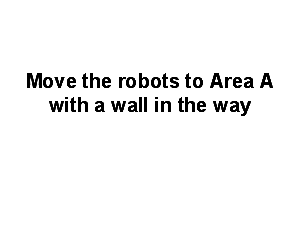
\includegraphics[width=\linewidth]{../ui_experiment/slide_images/Swarm_Robot_Control_-_10_Robot_0004.png}
	\end{subfigure}
	\begin{subfigure}{0.4\textwidth}
		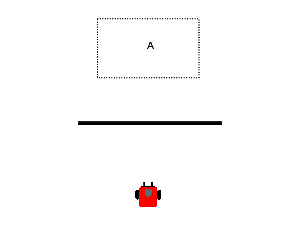
\includegraphics[width=\linewidth]{../ui_experiment/slide_images/Swarm_Robot_Control_-_Single_Robot_0005.png}
	\end{subfigure}
	\begin{subfigure}{0.4\textwidth}
		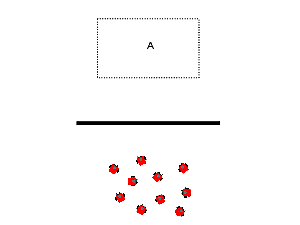
\includegraphics[width=\linewidth]{../ui_experiment/slide_images/Swarm_Robot_Control_-_10_Robot_0005.png}
	\end{subfigure}
	\begin{subfigure}{0.4\textwidth}
		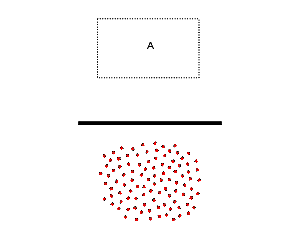
\includegraphics[width=\linewidth]{../ui_experiment/slide_images/Swarm_Robot_Control_-_100_Robot_0005.png}
	\end{subfigure}
	\begin{subfigure}{0.4\textwidth}
		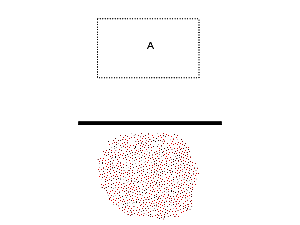
\includegraphics[width=\linewidth]{../ui_experiment/slide_images/Swarm_Robot_Control_-_1000_Robot_0005.png}
	\end{subfigure}
	\begin{subfigure}{0.4\textwidth}
		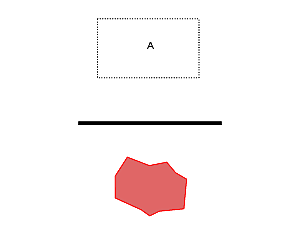
\includegraphics[width=\linewidth]{../ui_experiment/slide_images/Swarm_Robot_Control_-_Unknown_Number_of_Robots_0007.png}
	\end{subfigure}
	\caption{Instructional slide and situations for moving around the wall to area A, in each condition.}
	\label{fig:move_around_wall}
\end{figure}

\begin{tabular}{l|l|l|l|l|l}
& 1 & 10 & 100 & 1000 & Unknown \\
Move to area A & x & x & x & x & x\\
Move to area A with a wall & x & x & x & x & x \\
Stop the robots & x & x & x & x & x\\
Divide around an obstacle & & x & x & x & x \\
Orange to B, red to A & x & x & x & x & x \\
Orange to A, red to B & x & x & x & x & x \\
Orange to A, red to B (mixed) & x & x & x & x & x \\
Divide group & x & x & x & x & x \\
Merge groups & & x & x & x & x \\
Form a line & & x & x & x & x \\
Form a square & & x & x & x & x \\
Move the crate to area A & x & x & x & x & x \\
Move the crate to area A (dispersed) & x & x & x & x & x\\
Mark defective robot & x & x & x & x & \\
Remove defective robot & x & x & x & x &  \\
Patrol the screen border & x & x & x & x & x \\
Patrol area A & x & x & x & x & x \\
Disperse over screen & x & x & x & x & x \\
\end{tabular}

The individual robot case is lacking the tasks that do not make sense for a single robot. A single robot cannot, for example, divide around an obstacle or form a square. 
The ``Merge groups" task was left out of the single robot case because of the potential for confusion when referring to a single robot as a group. 

The unknown number of robots condition has the same tasks as the 10, 100, and 1000 robot cases, except for the ``Mark defective robot" and ``Remove defective robot" task. 
Without UI elements that represent individual robots, the user cannot take any actions that refer to a specific robot. 

\subsection{Analysis} \label{section:Analysis}

User gestures were coded using a methodology adopted from the social sciences, Grounded Theory \citep{glaser2017discovery}.
Grounded Theory is an iterative process, where the data are first coded at a very fine-grained level, and then the resulting coded elements are compared to each other to try to determine their qualities, similarities, and differences. 
Codes can be consolidated or divided until repeated passes of coding and comparison no longer alter the emerging structure of the coding scheme. 
During each iteration of coding and comparison, the coder makes memos as well, describing the links they see between related coded elements and higher-level abstractions that relate the elements. 
These memos are eventually written up as the social scientific theory, which is believed to be grounded in the data because it arises from the coding process. 

\subsubsection{Initial coding pass} \label{section:Initial_coding_pass}

The inital pass used open coding, where the ``codes'' were essentially free-form text entry. 
Rough counts of the open codes for the first 10 participants indicated that ten of the codes covered 81\% of the 580 total coded events. 
The ten most heavily used codes are, in order of occurrence: drag, tap, voice command, box select, 2 finger drag, double-tap, lasso, tap and hold, 2 handed drag, reverse pinch, and parallel hands. 
This pass of coding indicated that a majority of the user actions could be coded as some form of drag, some form of tap, box or lasso selection, pinch, and parallel hands. 
The final gesture, ``parallel hands'' is placement of the hands, palms facing each other, over some area of the screen. This gesture was used many times by the same user who issued voice commands, to indicate where the robots should form a line. Because parallel hands only accounted for 0.69\% of the gestures, it was left out of the development of the coding application for the second stage of coding. 

The most common code was drag, which accounts for 37.58\% of the rough coding, or 42.07\% if all forms of drag in the top ten codes are considered. ``Drag'' is when the user places one finger down, moves it to another location, and raises it again. Two finger drag is the same, only with two fingers on the same hand placed on the screen rather than one. Two-handed drag is single-finger drag, but executed with both hands at the same time. 

The second most common code was ``tap'', with 20.34\% of the rough coding, or 25.34\% if tap, double-tap, and tap and hold are all considered. Tap is when the user places a finger down and then very quickly raises it again. Double-tap is two taps in the same location in quick succession. Tap and hold is when the user places their finger on the screen and leaves it in one place for more than a second before raising it. 

Box select consists of a diagonal (relative to the screen edges) drag gesture over the robots or another object on screen, with the intent to select everything within the box whose diagonal is represented by the drag. 
Lasso select is a drag which ends near where it began, forming a loop, with the intent to select everything inside the loop. 

Pinch and reverse pinch are essentially two-hand drag or two-fingered drag but with the hands or fingers moving towards (pinch) or away (reverse pinch) from each other.
This gesture is common for zooming in multitouch user interfaces on smartphones. 

Voice command was used to code when a user spoke a command out loud, rather than using gestures. The high incidence of voice commands (7.07\% of all codes) in the first ten users can be attributed to a single user who issued commands almost exclusively through voice. 
 
\subsubsection{Second Coding Pass} \label{section:Second_Coding_Pass}

To facilitate coding in the second pass, an application was developed to record codes. 
The application has coding functions for the six most common gestures: drag, tap, voice command, box select, lasso select, and pinch. 
It also includes coding functions for user interface elements described by the user, such as buttons or menus, a function to code user gestures not covered by the six most common gestures, and a function for coders to enter free-form text memos. 

\todo{Need to make the call as to whether example gestures that users made should be counted along with ``real'' gestures, or left out. Maybe go both ways and see if it affects anything.}

A second pass of coding of the first ten user recordings was performed by two coders. 
Because the coders were responsible for deciding which user actions to code, as well as how to code them, it is possible for one coder to miss a gesture that another coder codes, or to split a single gesture into two coded units instead of one. 
For example, one coder initially split spoken commands at conjunctions such as "and", resulting in two units both coded as voice commands, while the other coder coded the entire sentence as a single unit. 
This leads to the possibility that for a single task, the coders will produce different length lists of coded units. 

Cohen's $\kappa$ is a measure of inter-coder reliability for categorical items, but it assumes that both coders are coding the same number of codable units \citep{cohen1960coefficient}. 
In order to calculate inter-coder reliability in the presence of potentially missing data, the  shorter of the two lists of codes for each task padded with a code for ``no data". 
The codes were then aligned chronologically, with pair consisting of an item from each list such that the total time error within the task was minimized.
As a result, the alignment process created pairs of a valid code and the ``no data" code for the codes in the longer list that did not have a good chronological match in the shorter list.
This was based on the assumption that the source of the error is one coder missing an event that did occur, rather than the other coder coding an event that did not occur. 

The initial pass of coding got poor inter-coder reliability, with the first 10 participants having Cohen's $\kappa$ of 0.357, 0.266, 0.398, 0.387, 0.643, 0.428, 0.407, 0.56, 0.273, and 0.502. 
Cohen's $\kappa$ of over 0.75 is excellent agreement, 0.4-0.75 is fair, and below 0.4 is poor, so the average $\kappa$ was barely above the cutoff for fair agreement. 

Analysis of the data, particularly with confusion matrices, showed several problems. 
The simplest was training error in the training of the coders.
One coder had not been instructed that the ``UI'' code existed, and so had coded user interface widgets as ``tap'' events.   
This was immediately apparent in the confusion matrix as a very high confusion between ui and tap events. 
The other main source of confusion was lasso and box selection actions being coded as drag events, and vice versa.
The actual action performed in a lasso is a drag, in that the user puts their finger down and drags it in a circle around something before lifting it again, but it is intended as a selection of the things inside the circle rather than e.g. drawing a circle shape. 

In order to reduce these errors, and ensure consistency in training the coders, the descriptions for each code were written up in discussion with the coder, so that questions about interpretations could be answered in advance and recorded. 
Another coder was trained with the code description document, and coded the first 5 participants. 
This coder obtained Cohen's $\kappa$ of 0.728, 0.927, 0.75, 0.827, and 0.738 with one of the original coders.
These values indicate a very high level of agreement, so the remaining videos were coded by these two coders, using the description of the codes from the code description document.  

The resulting data set has 3,256 individual gestures coded. 
In coding, the codes were box selection, lasso selection, drag, tap, pinch, ui widgets, voice command, and other. 
\todo{Insert text of coding document}
For analysis, drags that were used to draw something on the screen were separated from non-drawing drags. 
Taps were separated into single, double, and triple taps, plus tap and hold. 
Pinch was separated into pinch (where the contact points move towards each other) and reverse pinch (where the contact points move apart).
All of these divisions were based on modification flags used during the coding process.  

\begin{tabular}{l r r}
gesture & count & percent\\
drag & 1084 & 33.2924 \\
draw & 761 & 23.3722 \\
tap & 514 & 15.7862\\
other & 189 & 5.8047 \\
lasso & 184 & 5.6511 \\
box & 113 & 3.4705 \\
ui & 112 & 3.4398\\
double tap & 95 & 2.9177 \\
hold & 66 & 2.0270\\
reverse pinch & 49 & 1.5049 \\
voice & 44 & 1.3513\\
pinch & 26 & 0.7985 \\
triple tap & 19 & 0.5835\\
\end{tabular}

\section{Selection Gestures} \label{section:Selection_Gestures}
One area in which the gestures were expected to change between conditions is the use of selection gestures. 
The intuition behind this expectation is that for small numbers of robots, there is no need for a gesture that selects groups, as the user can interact directly with each robot. 
Similarly, in the case where no individual robots are displayed, the use of group selection gestures would be minimal, as the group is presented as a single cloud. 

Users performed selection of robots in groups by box select, lasso, and UI interactions.
These selections were counted by condition by counting lasso or box events that had a robot or robots as their targets. \todo{The std dev for a lot of these is bigger than the data, very high variability. Discard outliers? There are only ten users per condition to begin with}
 
\begin{table}
	\centering
	\begin{tabular}{l r r r r}
		Condition & Box Select & Lasso & Tap & Total (condition)\\
		\hline
		unknown & 0 & 1 & 43 & 44 \\
		one & 0 & 3 & 78 & 81\\
		ten & 26 & 105 & 140 & 271\\
		hundred & 68 & 53 & 35 & 156\\
		thousand & 18 & 16 & 22 & 56\\
		\hline
		TOTAL & 112 & 178 & 318 & 608\\
	\end{tabular}
	\caption{Per-condition total use of selections}
\end{table}

Single selections of robots were performed by tapping on the robot. 
Similarly to the count of group selections, tap events were counted where the object of the tap event was a robot or robots. 

The ten robot case has the most selection gestures for either group or single selection. 
As was expected, the unknown number and single robot cases have very low counts of group selections. 
Interestingly, the thousand robot case also has relatively low group and single 
selection use, especially compared to the ten robot case. 

To determine if these differences were statistically significant, the count of each user's gestures per task were normalized by dividing by the total number of gestures that that user used to perform the task. 
Normalizing in this manner converts raw gesture counts to a proportion of the total gestures used on that task, which prevents more verbose users from dominating the analysis.

The tasks checked for statistically significant differences between conditions were those that all conditions had in common. 
These nine common tasks are `move crate', `divide by color (cross)', `divide by color', `move to a', `move to a (wall)', `patrol a', `patrol screen', `split', and `stop'. 
Across all the common tasks the proportions of each gesture were collected per gesture, resulting in, for each gesture, 5 lists, one for each condition. Each list consists of 90 entries, 10 users times 9 common tasks. Each list entry consists of the proportion of that gesture the user used to complete the task. ANOVAs were performed for each pair of conditions. 

% This is PER-USER normalization, but PER TASK normalization is what I want
%For uses of tap as selection across the common tasks, the unknown number condition differs from the hundred (F=8.8744, p=0.0033) and thousand (F=4.8577, p=0.0288) robot conditions. 
%The one robot condition differs from the ten (F=4.5036 , p=0.0352), hundred (F=13.7996 , p=0.0003) ), and thousand (F=10.4596, p=0.0014) robot conditions.
%The ten robot condition differs from the hundred robot condition (F=4.2012, p=0.0419).
%These differences are summarized in table \ref{tab:tap_select_per_user_norm}.
%
%\begin{table}
%	\begin{tabular}{l|l l l l l}
%		& unknown & one    & ten        & hundred     & thousand   \\ 
%		\hline
%		unknown & & 0.1066 & 0.4915 & \textbf{0.0033} & \textbf{0.0288} \\   
%		one & & & \textbf{0.0352} & \textbf{0.0003} & \textbf{0.0014} \\
%		ten & & & & \textbf{0.0419} & 0.1828   \\
%		hundred & & & & & 0.3132   \\
%		thousand & & & & &\\
%	\end{tabular}
%	\caption{p-values for the use of tap as select between conditions}
%	\label{tab:tap_select_per_user_norm}
%\end{table}

For uses of tap as selection across the common tasks, the unknown number condition differs from the hundred (F=7.6964, p=0.0061) and thousand (F=5.5772, p=0.0193) robot conditions. 
The one robot condition differs from the ten (F=4.3299, p=0.0389), hundred (F=13.5889, p=0.0003), and thousand (F=10.4274, p=0.0015) robot conditions.
These differences are summarized in table \ref{tab:tap_select_per_user_norm}.

\begin{table}
	\begin{tabular}{l|l l l l l}
		& unknown & one    & ten        & hundred     & thousand   \\ 
		\hline
		unknown & & 0.5622 & 0.1772 & \textbf{0.0006} & \textbf{0.0193} \\   
		one & & & \textbf{0.0389} & \textbf{0.0030} & \textbf{0.0015} \\
		ten & & & & 0.1089 & 0.2719   \\
		hundred & & & & & 0.5457   \\
		thousand & & & & &\\
	\end{tabular}
	\caption{P-values for the use of tap as select between conditions}
	\label{tab:tap_select_per_task_norm}
\end{table}

For uses of group selection across the common tasks, the unknown number condition differs from the ten (F=47.635915, p<0.0001), hundred (F=60.435124, p<0.0001) and thousand (F=10.2346959, p=0.0016) robot conditions. 
The one robot condition differs from the ten (F=47.6359, p<0.0001), hundred (F=60.4351, p<0.0001), and thousand (F=10.2347, p=0.0016) robot conditions.
The ten robot condition differs from the thousand robot condition (F=19.0110, p<0.0001).
The hundred robot condition differs from the thousand robot condition (F=30.2373, p<0.0001).
The identical F and p values for the one and unknown robot conditions and the various conditions that they differ from are because for the one and unknown robot conditions, no group selection gestures were used in the common tasks. 
These differences are summarized in table \ref{tab:group_select_per_task_norm}.

\begin{table}
	\begin{tabular}{l|l l l l l}
		& unknown & one    & ten        & hundred     & thousand   \\ 
		\hline
		unknown & & * & \textbf{0.0000} & \textbf{0.0000} & \textbf{0.0016} \\   
		one & & & \textbf{0.0000} & \textbf{0.0000} & \textbf{0.0016} \\
		ten & & & & 0.1808 & \textbf{0.0000}   \\
		hundred & & & & & \textbf{0.0000}   \\
		thousand & & & & &\\
	\end{tabular}
	\caption{P-values for the use of group selections between conditions. The ANOVA between the unknown case and the single robot case was not computable, as no group selections were used for the unknown case or the single robot case for the common tasks.}
	\label{tab:group_select_per_task_norm}
\end{table}

\begin{table}
	\begin{tabular}{l | l l}
		& common tasks & all tasks\\
		\hline
		unknown & 0 & 1\\
		one & 0 & 3\\
		ten & 55 & 107 \\
		hundred & 60 & 109\\
		thousand & 15 & 28\\
	\end{tabular}
	\caption{Counts of group selection gestures in the common tasks and all tasks.}
	\label{tab:group_raw_counts}
\end{table}

\begin{table}
	\begin{tabular}{l | l l}
		& common tasks & all tasks\\
		\hline
		unknown & 15 & 29\\
		one & 38 & 53 \\
		ten & 45 & 108\\
		hundred & 4 & 29 \\
		thousand & 7 & 18\\
	\end{tabular}
	\caption{Counts of tap selection gestures in the common tasks and all tasks.}
	\label{tab:tap_raw_counts}
\end{table}

Examining the non-normalized counts of taps as selections and group selections across both the common tasks and all tasks indicates that heaviest use of tap selection is in the ten robot case. Heaviest use of group selection is in the hundred robot case, but the ten robot case only lags it by two uses. The second heaviest for group selection is the hundred robot case, while the second heaviest for tap selection is the single robot case. This seems to indicate that with single robots, users prefer tap selection, with one hundred robots they prefer group selection, but with ten robots, either selection method could be viewed as appropriate. 

It was surmised that users may have been performing multiple tap selections in a row to select robots in the ten robot case, but that a 10-robot tap selection would be condensed by the normalization into the same proportion of the overall gestures as a single-robot tap selection. 
To check if users were performing multiple taps in a row as selections, the lengths of sequences of tap actions were checked across all cases. 
As seen in table \ref{tab:tap_seq_len}, while the ten robot case does have a much higher count of sequences of taps, the mean is higher than the other cases, and the standard deviation much higher. 
On examining the data, there was exactly one case of a 10-tap sequence in the ten robot case.
While it is possible that a user in the ten-robot case might perform a selection by tapping each of the ten robots, but it is not a common occurrence. 

\begin{table}
	\begin{tabular}{l | l l l}
		& Sequence Count & Mean Length & Standard Deviation \\ 
		\hline
		unknown & 28 & 1.0357 & 0.1856 \\
		one & 42 & 1.2619 & 0.5798\\
		ten & 72 & 1.5000 & 1.6499\\
		hundred & 23 & 1.2609 & 0.4391\\
		thousand & 17 & 1.0588 & 0.2353\\
	\end{tabular}
	\caption{Lengths of sequences of taps within conditions.}
	\label{tab:tap_seq_len}
\end{table}

% TRIPLE CHECK THIS BEFORE USING ANY OF IT
%For the box selection gesture, the unknown condition differs significantly ($\alpha$ = 0.05) from the ten (F=7.17386 p=0.00809), hundred (F=26.95175 P=0.00000), and thousand (F=4.57743 p=0.03376) robot conditions, but not from the single robot condition (F and p values could not be calculated due to disuse of box selection in these cases). 
%The use of box select in the one robot condition differs significantly from the ten (F=7.17386 p=0.00809), hundred (F=26.95175 p=0.00000), and thousand (F=4.57743 p=0.03376) robot conditions.
%The hundred robot condition differed from the ten (F=9.17884 P=0.00281) and thousand (F=13.81053 P=0.00027) robot cases. 
%
%
%
%For the lasso gesture, the unknown condition differs significantly from the ten (F=33.27742 P=0.00000), hundred (F=19.44664 P=0.00002), and thousand (F=5.86234 P=0.01647) robot cases. 
%The one robot condition differs significantly from the ten (F=33.27742 P=0.00000), hundred (F=19.44664 P=0.00002), and thousand (F=5.86234 P=0.01647) robot cases as well. \todo{Why are these differing by the same amount between unknown and one? The same proportions?}
%The thousand robot condition also differed from the ten (F=23.51414 P=0.00000) and hundred (F=11.76321 P=0.00075) robot conditions. 
%
%For the tap gesture, the unknown condition differs significantly from the one (F=5.07967 P=0.02543) and thousand (F=5.31693 P=0.02227) robot conditions. 
%The one robot condition differs from the ten (F=5.58672 P=0.01918), hundred (F=7.47952 P=0.00687), and thousand (F=21.15146 P=0.00001) robot conditions. 
%The thousand robot also differs from the hundred robot condition (F=4.08954 P=0.04465), although not as strongly as many of the others. 
%However, this analysis looks at all uses of tap, not just tap intended as select, as detected by the object of the tap being a robot.
%
%To determine if tap-as-select, rather than just any use of tap, maintained this relationship, the count of group selects (box or lasso with robots as the object) and single selects (taps with robots as the object), were collected, per user across all tasks that are common to all conditions. 
%These lists were averaged, to get the average use of group select or single select, for each task, averaged across the condition.\todo{This is raw counts, should maybe do this and then normalize to get proportions, rather than average.}
% 
%For tap-as-select, the hundred robot case differed from the unknown (F=5.61783, p=0.03068), one (F=9.13207, p=0.00810) , and ten (F=6.59643, p=0.02062) robot cases. The thousand robot case differed from the ten (F=5.64536, p=0.03033) and one (F=7.62757, p=0.013893) robot cases.
%
%For group select, the hundred robot case differed from the unknown (F=5.61783, p=0.03068), one (F=9.13207, p=0.0081) , and ten (F=6.59643, p=0.02062) robot cases. The thousand robot case differed from the ten (F=5.64536, p=0.03033) and one (F=7.62757, p=0.01389) robot cases.



%The gestures draw, pinch/reverse pinch, and double-/triple-tap did not display any statistically significant difference across conditions in the common tasks. 
%Pinch/reverse pinch were somewhat task-specific gestures, used across condition to divide/merge groups of robots in that task. 
%
%Draw is also somewhat task specific, mostly used in formations to draw the target shape. However, the formation tasks are not in the common task set, because a single robot cannot form a formation. 
%
%Were double and triple taps also specific to some task? This would be interesting to check, because it seems to indicate a division of gestures into gestures that were related to a task, and gestures that were related to a condition. 
%
%Graphing \todo{put the graphs in here} average per-user proportion of gestures per task indicates that pinch or reverse pinch were highest in divide color 1, patrol a, patrol screen, and split. Split had by far the most reverse-pinch gestures. 
%
%Draw peaked for split and stop. For split, this was caused by users drawing a dividing line between the split groups. For stop, it was caused by users drawing a line in front of the robots to indicate a virtual barrier. If the formation tasks were in the common task set, they would also likely have large numbers of draw gestures. 
%
%Doubletap peaked in the stop case as well, but triple taps occured at a very low level in crate, divide color 1, and move a, and at a slightly higher level in patrol screen and split. In general, tripletap may not have enough samples to make a comparison meaningful. It was only used 19 times total, and is the least common gesture. 

[DATA INTENSIFIES]

\section{Multi-hand Gestures}

Multi-hand gestures fall into two different groups. \
The first group is gestures where each hand is performing part of a single gesture.
Generally, these were pinches and reverse pinches with one finger on each hand. 
%[PUT COUNT HERE] users also performed two-handed drags with one finger of each hand. 
The other group of multi-hand gestures consists of a simultaneous pair of different gestures, one performed with each hand. 
For purposes of coding, dragging one object to one place with two fingers was coded as a single drag with two fingers, while dragging two objects to two different places was coded as two single-fingered drags at the same time. 

Fifty percent of the users performed at least one two-handed gesture. 
This is fewer than in some previous research, but more than might be expected if users were generalizing from single-point mouse interaction \cite{micire2010multi, epps2006study}
Epps et al required users to use a single hand for over half of the gestures in their study, and they point out that their use of a Windows desktop as the working environment of the study may have influenced people towards a single-point interaction style. 

There were 82 instances of two-handed gesturing. 
If this total is treated as 164 gestures, one for each hand, two-handed interactions account for 5.037\% of the gestures used.

%u'box_select box_select': 3,
%u'box_select tap': 1,
%u'box_select ui': 1,
%u'drag drag': 26,
%u'drag tap': 4,
%'drag_s drag_s': 5,
%u'other other': 5,
%'pinch pinch': 22,
%'reverse_pinch reverse_pinch': 7,
%u'tap drag': 2,
%u'tap tap': 6
\begin{table}
	\centering
	\begin{tabular}{l l}
		Gesture Pair & Count\\
		\hline
		drag and drag (different objects) & 26 \\
		pinch & 22\\
		reverse pinch & 7\\
		tap and tap & 6\\
		drag and tap & 6\\
		drag (same objects) & 5\\
		other and other & 5\\		
		box select and box select & 3\\
		box select and tap & 1\\
		box select and UI & 1\\
		\hline
		TOTAL & 82\\
	\end{tabular}
	\caption{Two handed gesture pairs. Note that the total is lower than the actual count of total gestures, since it counts e.g. two simultaneous drag actions as a single two-handed drag action.}
\end{table}

Most of the two-handed gestures were simultaneous drags of two different objects. 
Simultaneous drags and two handed pinches or reverse pinches account for 58.537\% of the two-handed gestures.  

Due to the prevalence of smartphone adoption, it is no longer simple to determine if smartphone use contributes to the use of pinch and reverse pinch gestures, because there are almost no smartphone non-users in the population of this study. 
Out of 50 subjects, 46 (92\%) reported using an Android or Iphone smartphone daily. 
Only one user did not report having used an Android or Iphone at least moderately, and stated that they did not own any touchscreen devices. 
Despite not having any touchscreens, even this user made two-handed gestures. 

\begin{table}
	\centering
	\begin{tabular}{l l}
		Task & 2-Handed Gesture Count\\
		\hline
		merge&14\\
		divide&12\\
		square&12\\
		divide color 2&9\\
		patrol screen&9\\
		split&6\\
		divide color 1&5\\
		divide color mix&4\\
		move wall&4\\
		line&2\\
		move a&2\\
		crate&1\\
		disperse&1\\
		stop&1
	\end{tabular}
	\caption{Use of two-handed gestures by task.}
\end{table}

\todo{is number of hands used influenced by number of robots?}

\todo{use of handwriting as percentage of gestures}

\todo{Use of onscreen keyboards}

\subsection{Influence of Video Games}

Previous research had indicated that users of Real Time Strategy (RTS) games would be predisposed to the use of box selection gestures, because many RTS games use box selection to select areas of the screen or units to control \cite{micire2010multi}. 
Nine users reported playing RTS games, including Age of Empires, League of Legends, Supreme Commander 2, Civilization, and Europa Universalis. 
The count of per-task box selection gestures was collected, and divided between users who had played RTS games and those who had not. 
RTS users made 51 box select gestures, while non-RTS users made 49.
While these two totals are quite close, bear in mind that RTS players are less than one fifth of the total population, but used over one half of the box selection gestures. 
The mean per-task use of box selection among RTS users is 0.3828 (std. dev. 0.7408), and the mean use of box selection among non-RTS users is 0.0748 (std. dev. 0.3392). 
ANOVA results indicate that the difference is statistically significant (F=53.8527, p < 0.0001).
 
The use of user interface elements, such as menus or buttons on the screen, was also much higher in RTS gamers than non-RTS users. 
RTS-playing users made 74 UI gestures, while non-RTS users made 20. 
The average per-task use of UI gestures was 0.5781 among RTS users (std. dev. 1.8608) and 0.02932 (std. dev. 0.1853) among non-RTS users. 
ANOVA results indicate that the difference is significant (F=56.2048, p < 0.0001).

\subsection{Influence of Operating Systems}

For the disperse task, 12 users made a gesture that was similar across multiple users, consisting of placing four or five fingertips on the same hand together on the screen, and spreading them away from each other. 
Because a single robot cannot disperse, this task was only presented to users in the unknown, 10, 100, and 1000 robot cases, so 40 users saw this task. 
Several users compared the multi-finger scatter to a gesture to show the desktop or all the windows on a Macintosh computer, and Apple's multitouch help indicates that spreading the thumb away from three fingers on the touchpad of a Macintosh laptop will have this effect \citep{AppleTouchpadHelp}. 

Unfortunately, the possibility that a desktop OS might predispose users to a certain style of multitouch interaction was not considered, and so the post-test survey did not ask users what OS they were familiar with. Of the 12 scatter gesture users, 8 reported familiarity with other Apple iOS devices, but this should not be taken to imply that they were familiar with the Mac OS multitouch gestures. 

\subsection{Use of Voice Commands}

Twenty percent of the users (10 users) used voice commands. 
Only one user used voice commands for all of their interactions. 
Over all of the tasks, voice commands were used for the formation tasks, `line' (5 commands) and `square' (4 commands), more than any other task. 
This is likely due to a bias inadvertently created by colloquial use of the verb ``tell'' in the instructional slides for the formation tasks.  
The instructional slides read ``Tell the robots to form a line/square", and some users read this to mean that they should speak the words ``Form a line" or ``Form a square", addressed to the robots.

The `stop' task also was performed with a voice command by three users. 
Users indicated that even if they hadn't otherwise been using voice commands, the users would use them for the task of stopping the robots. 
Since this task assumes the robots are already moving towards a goal, users stated that attempts to interact with all of them by using gestures while they are moving could be difficult. 

The `divide color mix' task was also performed by voice command by three users. 
This task requires some form of selection by color to separate robots that are in a mixed group, so users would assume that robots knew their color, and address them with commands such as ``red robots, unite".

Overall, the 20\% use of voice commands is much higher than the 1.3\% observed in a previous study \citep{micire2010multi}. 
While that study took place as smartphones were becoming popular (and observed effects related to smartphone experience), this study was performed after the introduction of Google Now/Assistant (2012/2016), Microsoft Cortana (2014), Amazon Alexa (2014), and Apple Siri (2011). 
Aside from Alexa, these voice assistants are all accessed through smartphones.  
All of the users of voice commands reported high familiarity with Android or IPhone smartphones, but the survey did not ask if they used the voice assistant feature of their phones. 
As a result, no conclusion can be drawn about the influence of voice assistant technology on user interface expectations from this study. 


%For the task of removing the defective robot, the location selected for it to be removed to was usually either a corner, a ``recycle bin" or similar disposal area, or off the edge of the screen. This use of the area beyond the screen for placement of deleted or rejected things parallels that seen by Wobbrock \textit{et al} \citep{wobbrock2009user}.
%
%Some users reused gestures for different purposes, such as tapping a robot to select it, but also tapping a robot to remove it.
%Because the users could not be expected to choose a consistent gesture set for an \emph{a priori} unknown set of tasks, this sort of inconsistency is not unexpected. 

\subsubsection{Robot Count in Unknown Number Case} \label{section:Robot_Count_in_Unknown_Number_Case}

In the condition where the exact number of robots was unknown, and the swarm was depicted as a cloud, participants were asked to say how many robots they felt the cloud represented. 
Generally, the participant expectation was that the cloud represented tens of robots, but simply averaging the responses would not be useful, as one participant said that it ``could be millions''. 
For those that did answer with a single number or range, the answers were 10-20, 10-``hundreds'', 12, 7, 10, 2-10, 10-12, 2-``millions', 5-10, 8, and 50. 
If the endpoints of ranges are treated as answers, with ``hundreds'' and ``millions'' set to 500 and 5,000,000 respectively, the median answer is 10, but the mean and standard deviation are not illustrative of the user responses. 
Rejecting ``hundreds'' and ``millions'' as outliers gives a mean of 11.86, with a standard deviation of 11.04, which adequately covers the common intuition that the swarm contains at least 2 members and many have tens, but not likely hundreds, of robots in it.

Participant comments may shed some light on the source of this intuition. 
One participant indicated during the study that they interpreted the corners of the polygonal cloud as possible robot locations, and so drew an idea of the scale of the swarm from the number of corners. 
The cloud has 11 corners, 7 convex and 4 concave, which is consistent with the estimated robot count. 
Another participant said their estimate was informed by the instructional slides preceding the test, which depicted a number of robots, the outline around them, and the resulting cloud, as shown in fig. \ref{instructional slides}. 
These slides depicted 10 robots, and so may have biased participants to expect that the cloud had 10 robots in it. 
However, multiple participants stated that the cloud represented an unknown number, or estimated more or less than 10 robots.

\begin{figure}
	\centering
	\begin{subfigure}{0.3\textwidth}
		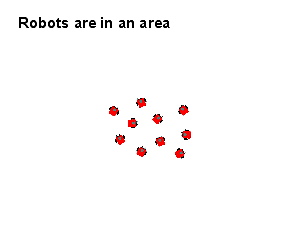
\includegraphics[width=\linewidth]{../ui_experiment/slide_images/Swarm_Robot_Control_-_Unknown_Number_of_Robots_0001.png}
	\end{subfigure}
	\begin{subfigure}{0.3\textwidth}
		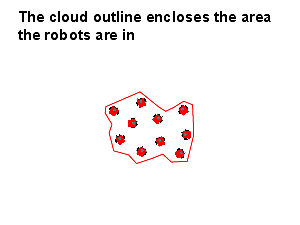
\includegraphics[width=\linewidth]{../ui_experiment/slide_images/Swarm_Robot_Control_-_Unknown_Number_of_Robots_0002.png}
	\end{subfigure}
	\begin{subfigure}{0.3\textwidth}
		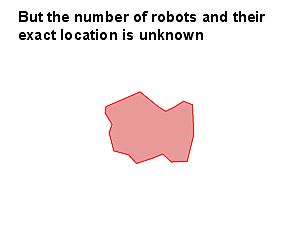
\includegraphics[width=\linewidth]{../ui_experiment/slide_images/Swarm_Robot_Control_-_Unknown_Number_of_Robots_0003.png}
	\end{subfigure}
	\caption{Instructional slides for the unknown number of robots condition, showing cloud representation of robot swarm.}
	\label{instructional_slides}
\end{figure}

\subsubsection{Selection Strategy} \label{section:Selection_Strategy}

At the end of the experiment, users were shown an image of a robot swarm, with a dotted line around it depicting a finger drag path around some of the robots. 
The users were told that the intent of this gesture was to select robots, and asked to indicate which robots in the image were selected, or in the unknown number of robots case, whether the gesture selected all of the robots or left any out. 
Users in the single robot case were shown the selection image with ten robots in it, because the with one robot, there are not enough robots to have a selection which may exclude some robots and include others. 

\begin{figure}
	\centering
	\begin{subfigure}{0.48\textwidth}
		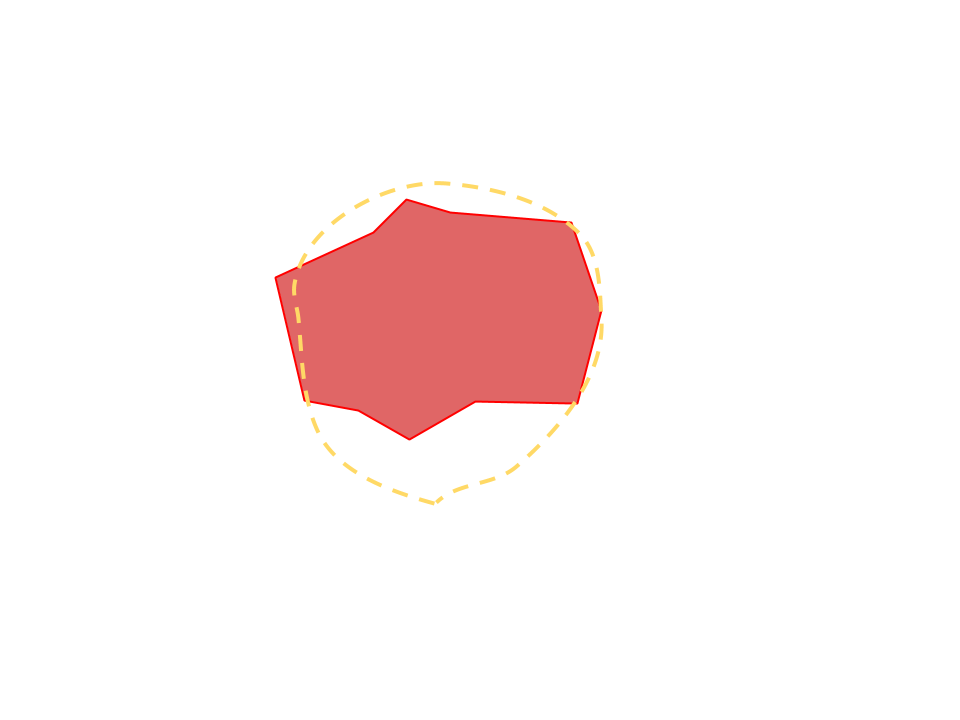
\includegraphics[width=\linewidth]{../Selection_Fuzz_X.png}
	\end{subfigure}
	\begin{subfigure}{0.48\textwidth}
		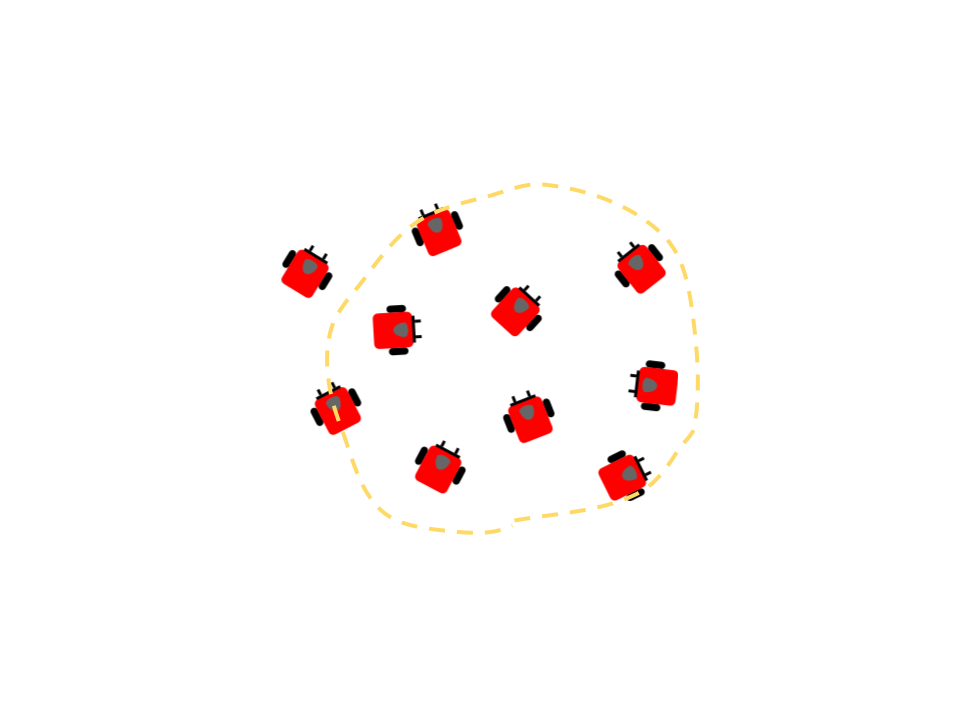
\includegraphics[width=\linewidth]{../Selection_Fuzz_10.png}
	\end{subfigure}
	\begin{subfigure}{0.48\textwidth}
		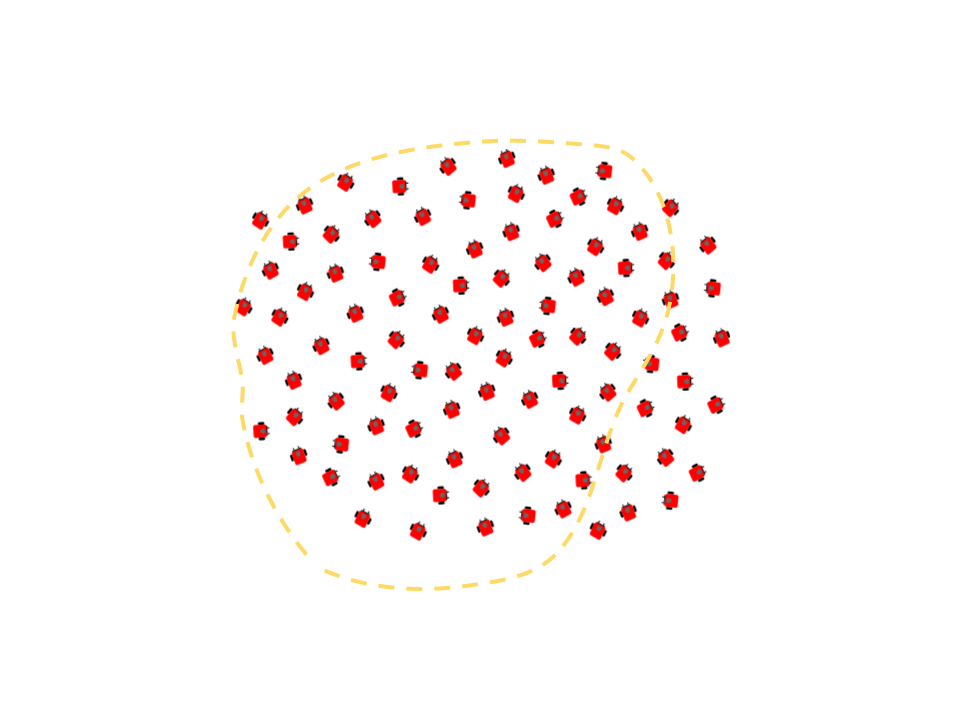
\includegraphics[width=\linewidth]{../Selection_Fuzz_100.png}
	\end{subfigure}
 	\begin{subfigure}{0.48\textwidth}
		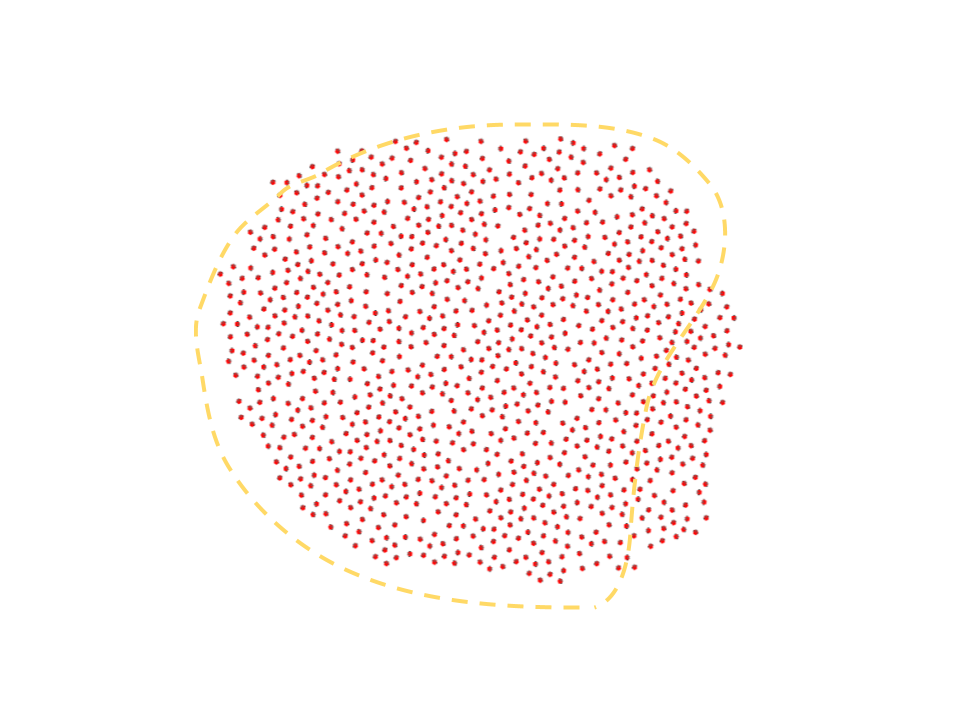
\includegraphics[width=\linewidth]{../Selection_Fuzz_1000.png}
	\end{subfigure}
		\caption{Images for selection strategy question.}
	\label{strategy_question}
\end{figure}

In the unknown number of robots case, 7 participants indicated that all the robots were selected, 3 of the participants indicated that some robots were left out, and one participant indicated that whether the selection included all of the robots could depend on the task. 

Because the 1 and 10 robot cases saw the same selection image, they are reported together. 
12 participants indicated that robots that were inside the selection or touched by the selection line should be considered selected. 
2 participants indicated that robots depicted with half or more of the robot inside the circle should be considered selected. 
One participant indicated that the robot half out of the circle should \emph{not} be selected. 
One participant indicated that robots on the border should be included or not included in the selection, depending on the task. \todo{Three answers are missing, find those and fix}
One user indicated that only the first robot touched should be selected, which is consistent with control strategies that move each robot individually. 

For the hundred robot case, 3 participants indicated that robots inside or touching the line were selected. 
3 participants said that robots should be mostly inside the line to be counted, with one participant stating that robots should be 80\% or more inside the line to count. 
2 participants indicated that robots should be more than halfway inside the line to be selected. 
One participant stated that only robots completely inside the line should be counted. \todo{One answer missing, find and fix}
 
In the thousand robot case, 7 participants indicated that robots inside or touching the line should be selected. 
2 participants indicated that robots must be completely inside the line to be selected. 
1 participant indicated that robots mostly inside the line should be selected. 

Overall, participants generally err on the side of inclusion, rather than exclusion of robots from selection.
If a user interface is required to include or exclude ambiguous elements from a selection, it appears that including ambiguous elements will satisfy users. 
User comments also suggested that ways to amend selections before further commanding the robots would be desirable.

 \begin{tabular}{ l l l l l}
   Condition & Completely inside & Half or more in & Touching line & Other\\
   \hline
   10 & 0 & 2 & 12 & 3 \\
   
   100 & 1 & 5 & 3 & 0 \\
   1000 & 2 & 1 & 7 & 0\\
   \hline
   Totals & 3 & 8 & 22 & 2 \\
 \end{tabular}

%It is interesting to note that two participants, one from the unknown number of robots case, and one from the 10 robot case, said that in cases of ambiguous selection, the system should add or remove robots from the selection based on the task. 
%As the system cannot predict the task it is about to be commanded to perform, it is likely best to err on the side of selecting too many robots, rather than too few. 



\subsubsection{Participant Demographics} \label{section:Participant_Demographics}

The experiment had 50 participants, 10 in each condition. 28 of the participants were male, 22 were female. The average age of participants was 22.1 years, with a standard deviation of 3.16. 

These demographics are representative of the location that the study was performed, the campus of an American college. 
It has been suggested that research in psychology focuses too much on a population that is WEIRD (Western, Educated, Industrialized, Rich, and Democratic), and that the results of such studies may not generalize beyond that population \citep{arnett2008neglected}.
However, for the purposes of this study, particularly assessing the influence of smartphone use on expectations of user interface gestures, it is useful to have a population with significant experience using smartphones, which are a product of both rich and industrialized societies. 
It is not proposed that the results of this work generalize to humanity as a whole.  

\subsection{Conclusions} \label{section:Conclusions}

In future, it would be interesting to repeat this work with a condition that does not display the robots in the user interface at all. 
We expect that for conditions such as the ``move the crate'' tasks, the user would simply indicate the crate should move to area A, without concern for which robots perform the moving. 
However, such an interface would not afford indicating particular robots or groups, so tasks such as dividing the robots around an obstacle may become impossible to perform.

During this experiment, there were some cases where the users expectations of what was possible in the interface indicated a sort of ``metaphor failure" in the user interface. 
Natural User Interfaces, of which multitouch screens are an example, are supposed to be able to leverage users' understanding of the physical world, and how objects behave in it, to build affordances for objects on the screen. 
For example, a volume knob can be displayed as an actual knob, and the screen can react appropriately to attempts to rotate the knob. 
However, people know that the objects on the screen are not e.g. knobs, switches, and so on, but pictures of those things, drawn by the computer. 
As a result, the affordances are mixed. 
The knob may afford turning, but it also affords dragging around the screen or deletion, which a knob on a real radio does not afford. 
In this study, users were tasked with stopping the robots, which had begun to move around a wall to a target area. 
One user dragged the wall in front of the robots, and another user asked if they could move the wall. 
The wall was intended to represent an actual wall, which doesn't afford moving in the physical world, but it was represented in the experiment as a thick black line. 
It may be that the users would have not attempted to move the wall if it was more clearly represented as e.g. a stone or brick wall, and so had connotations of excessive weight. 
On the other hand, the users may have regarded it as what it actually was, an image of a wall on a computer screen, and decided that since images can be moved around the screen, the wall image can too. 
Attempting to experimentally determine if the representation affects how the user interacts with the wall may require a large number of users, as out of 50 participants, only 2 even mentioned the idea of moving the wall. 

In this experiment, some users were initially confused by the interface not responding. 
It may be that running this experiment on a computer, rather than a paper prototype, contributed to the user expectation that the system could react. 
Most users' experience with touch screens is that when they touch them, something visible happens nearly immediately. 
A system that does not visibly react, as in this experiment, is usually assumed to be broken, or waiting for further input, but no one expects printed documents to react to touch.
For future work, it may be desirable to structure attempts to elicit user gestures as in Wobbrock \emph{et al.}. 
The experiment described in this section showed the initial situation, and asked the users how they would make a specific change. 
Wobbrock \emph{et al.} showed the change occurring, and then asked the users what command they would issue to cause that result. 
Showing the response before asking for the gesture removes the expectation that the system will react. 



%Where we're going, we don't need timelines
%\chapter{Timeline}

\section{September}

Gestures - The experiment to collect the gesture data set will be performed in September.   

Software - A preliminary gesture recognition system will be developed, although it may have to be amended to reflect the gestures collected in the experiment. 
Preliminary versions of the gesture compiler and the infrastructure for running the resulting programs on the robots are written, but they will be refined and extended.

\section{October}

Gestures - The experiment to collect the gesture data set will be completed, and analysis of the gesture data set will be done. 
The results will be written up and published if possible. 
At this point, it should be clear that there either is or is not a transition point where the user changes the gestures they use for a bigger swarm. 
If there is no transition, then it would seem to indicate that the same UI can be used for individual robots and swarms. 

Writing - Assuming data set for gestures is useful for a paper, it will be written up and published. The resulting write up, as well as expansion on experimental methodology will be added to my thesis. 

Software - The gesture recognizer will be extended with the gestures collected from the experiment.
Automation will be put in place to have the pipeline from gestures to program deployment on the robots occur without user intervention. 

\section{November}

As of this writing, the deadline to submit a Declaration of Intent to Graduate form for the fall is unknown (https://www.uml.edu/Registrar/Calendars/2017-fall-grad.aspx lists it as "TBD"), but it is likely in early December. It should be submitted sometime this month. 

Software - Finishing and cleanup work will be done on gesture compiler. It may be possible to connect the UI from the experiment to the overhead camera for the swarm, resulting in a complete overhead view interface for real robots. 

Writing - Notes on gesture compiler design and development will be added to thesis, and possibly developed towards a paper. Thesis defense presentation will be written.

\subsection{December}

Defend Thesis

Print copies of the thesis for submission to the library. 

As of this writing, the deadline to submit the thesis/dissertation to the library is unknown, but it is likely around the last day of fall semester classes, Dec 13th. 


\section{Expected Contributions}

\subsection{Multitouch Gesture set for Swarm Control}
This work will attempt to determine if there is an intuitive multitouch gesture set for a single user to command a large swarm of robots.
For the experiment, there are 5 cases: 1 robot, 10 robots, 100 robots, 1000 robots, and cloud (unknown robot count). 
In all the cases except the cloud case, the robots are represented as individual robots on the screen of the interaction device. 
In the cloud case, the robots are presented as a cloud covering the area that the robots are present in, but without precise representation of each individual robot. 

There are 18 tasks. 
Each user is assigned to one case, and then performs all the tasks using that case. 
Having each user work on one case is intended to prevent the user from being influenced by their memory of what they did in a different case, and so creating a consistency that is not a product of the requirements of the task and case. 
Some of the tasks do not make sense with the cloud case, such as interactions with a single robot, so users who are assigned to the cloud case will not view the tasks that are impossible in that case.
Pilot runs of the study indicate that it can be completed in one hour. 

The data set will be analyzed and compared to existing work on multitouch gestures for command and control. 
The analysis will also attempt to determine if the gesture set shows a transition point between many and few robots. 
The influence of the presentation of the interface on the gesture set will be examined. 
The gesture set will also be analyzed to determine if the size of the swarm has any effect on the gestures used, or on neglect of individual robots by the user. 

\subsection{Compilation of User Gestures into Robot Programs}
The automatic conversion from a user-specified task into a set of command programs to be distributed to the swarm robots is still an open question.
One recent approach uses a human-in-the-loop multitouch interface to allow a human to guide a swarm by drawing a bounding prism that the swarm attempts to remain within \citep{ayanian2014controlling}. 
As the bounding prism moves, the swarm moves with it, with the individual robots performing obstacle avoidance. 
However, this work assumes that the individual swarm units can localize themselves, and that there is constant availability of communications between all swarm members and the central controller. 
For a number of reasons, these assumptions frequently fail to hold, and so a more robust system can be designed by assuming that localization and communication are difficult. 
This work will attempt to create an automated process by which user-specified behaviors of the swarm as a whole can be converted into programs that run on individual robots. 
The behavior of the individual robots under this control should converge to the user-specified behavior without further communication from the central server.

Previous work in gesture control for small groups of robots was able to recognize a grammar of user inputs using a finite state machine \citep{micire2010multi}.
The intent of this work is to implement basic robot behaviors as statements in an implementation of guarded control programming with rates (GCPR), which can then be composed into more complex behaviors based on the recognized user gestures \citep{napp2011compositional}.  


\subsection{Inexpensive Swarm Hardware}

The previously described swarm robot platforms tend to fall into one of two groups, from a hardware perspective. 
The first group uses microcontrollers and very limited onboard computation, but is small and relatively cheap.
This group includes Alice, Jasmine, AmIR, and the other tabletop systems. 
Due to their limited computation, these systems do not generally support complex algorithms such as vision processing. 
The second group use more powerful computers, but at a significant cost in weight, power consumption, and financial outlay.

The robot described in this work is intended to occupy a theoretical ``sweet spot'' at the high end of the tabletop swarms or the low end of the room-scale swarms, depending on how large of a mobility platform is used. 
As a result, if it is configured for tabletop operation, the system can be used with a minimum of available space. 
If, on the other hand, it is configured for room-scale operations, the system can be tested in natural or naturalistic human environments. 

The robot swarm developed for this work consists of a hardware module for controlling two motors of a toy, such as a small RC car, for mobility. 
The reasons for choosing this hardware design are explained in more detail below, but the overall intent is to have an inexpensive platform available for swarm research, without having to rely on any particular group of swarm robotics researchers starting and maintaining a side business supporting and selling robots.
Duplication of software and other digital artifacts is trivial, so constructing a duplicate of the hardware becomes the primary difficulty. 
The use of toys for the mechanical components of the robots is intended to reduce the difficulty of constructing the hardware. 
If researchers are not to be expected to become entrepreneurs, they should also not be expected to become expert machine tool operators.
The hardware resulting from this work is designed so that it can be duplicated by a researcher using common tools, and possessed of no more than hobby-level familiarity with electronic hardware.

%\begin{figure}
%\centering
%\includegraphics[width=0.8\textwidth]{../robot_makers_2/tiny_tank}
%\caption{A tank-drive toy with a 3.7V lithium polymer battery and a control board mounted to it.}
%\end{figure}
%
%In order to be both heterogeneous and inexpensive, the robots used for this work are constructed by developing a Commercial Off-The-Shelf (COTS) modular control hardware platform that can be attached to children's toys. 
%Modified toys are an adequate substitute for custom mechanical assemblies, and permit easy experimentation with heterogeneous swarms. 
%The use of children's toys as mobility platforms may also avoid the sensitivity to the work surface exhibited by the Kilobots and, to a lesser extent, the Epucks.
%The controller module was designed to be used as a replacement for the control electronics of children's toys, similar to the Spider-Bots developed by Laird, Price, and Raptis, or Bergbreiter's COTSBots \citep{lairdspider, bergbreiter2003cotsbots}.
%However, unlike the Spider-Bots and COTSBots, this work does not specify a particular toy chassis to use for mobility. 
%Most children's toys use either one motor with a mechanical linkage to cause the toy to turn when the motor is reversed, or two motors.
%Two-motor toys frequently use either differential steering or have one motor provide drive power and the other provide steering. 
%All of these toys can be controlled by the hardware described in this work. 
% %
%The robots are intended to be heterogeneous, partly because of the advantages of heterogeneity in a swarm, and partly because toy supplies are unreliable.
%While toys in the general case are expected to remain available, a particular line of toys might be discontinued or a modified version released. 
%The software framework in development to support the robots is based on ROS, and so allows modular replacement of the control algorithms used to convert desired motion of the robot into drive signals for the motors. 
% %
%%Toys cost $24, $16, $15, $21/2, 
%\begin{table}
%	\begin{tabular}{l l l l}
%	Part & Price & Quantity & Subtotal\\
%	\hline
%	Mobile Toy & 14-20 & 1 & 20 \\
%	Battery & 2.54 & 1 & 2.54 \\
%	Main PCB & 2.75 &  1 & 2.75 \\
%	ESP8266 Module & 2-7 & 1 & 7.0 \\
%	DRV8830 & 2.30 & 2 & 4.60 \\
%	MIC5319-3.3YD5 & 1.36 & 1 & 1.36 \\
%	MCP73831 & 0.58 & 1 & 0.58 \\
% %	\hline
%	Total & & & 27.83-38.83\\
%	\end{tabular}
%	\caption{All prices are for single quantities of new parts. It may be possible to get bulk discounts, especially on the toys and ESP-8226 modules. The costs of the resistors and capacitors has been left off, as they cost fractions of a penny each.}
%\end{table}
% %
%The processor of the controller is an ESP-8266 wifi module.
%The ESP-8266 costs approximately \$3-5, and contains both a wireless interface and a micro controller that can be programmed from a variety of programming environments and languages, including Lua and the Arduino variant of C/C++. The ESP-8266 module is based on the ESP-8266 IC, made by Expressif Systems. The IC itself has an 80Mhz Tensilica Xtensa L106 processor with 64kB of instruction memory and 96kB of data RAM. The modules come equipped with 512kB to 16MB of flash memory for program storage, and some combination of the 16 GPIO lines of the IC available for use. 
%The ESP-8266 is available in several form factors, each designated by a different suffix. 
%The version selected is the ESP-8266-03, which offers more GPIO pins than most other versions, and includes an internal antenna.
% %
%In addition to 802.11 b/g/n WiFi, the ESP-8266 supports a variety of serial protocols, including a UART, I$^2$C, SPI. 
%The I$^2$C interface is used on the board to connect to two DRV8830 motor driver ICs by Texas Instruments. 
%The DRV8830 provides 1A of drive current.
%Experimental tests with 8 different toys indicate that small toys draw well under 1A while moving freely, and peak around 2A when the motors are stalled. 
%The tested toys include 3 insect-styled walkers, 3 wheeled vehicles (2 differential drive, 1 Ackerman steering), 1 toy helicopter, and 1 toy quadcopter.
%The DRV8830 provides overcurrent limiting, so a stall condition or short circuit of the motor leads will disable the motor drive, but not damage the DRV8830. 
% %
%The control module also provides connections for a 3.7V lithium-ion battery pack, as well as charge control circuitry for the battery. 
%The charge controller allows the robot to be charged from the same USB connection that is used to change the programming of the ESP-8266. 
%Reset and entry into programming mode is controlled by a separate USB-to-serial adapter board, the Sparkfun BOB-11736.
%Moving this functionality to the adapter board reduces the size and cost of the control module. 
% %
%\subsection{Toy Compatibility}
% %
%Children's toys normally use inexpensive brushed DC motors in their construction. 
%These motors have not been the subject of extensive study, as they are commodity parts. 
%However, it is useful to quantify their behavior to some extent, to determine which kinds of toys can be used with the controller. 
% %
%Two common types of motors found in children's toys are the RE and FA series of motors produced by Mabuchi Motor, or imitations of these motors produced by other companies. 
%These motors use simple metal brushes and are constructed to be inexpensive, rather than precise. 
%The intended voltage range of the motors varies with different winding types, but according to datasheets available from Mabuchi Motor, the voltage ranges and current draws for motors in this range are as shown in table \ref{tab:properBrandedMotors}.
% %
% %\begin{table}
%	\begin{tabular}{l l l l l}
%	Model & Voltage & No Load Current & Max Efficiency & Stall Current\\
% %	\hline
%	RE-140RA-2270 & 1.5-3 & 0.21 & 0.66 & 2.1 \\
%	RE-140RA-18100 & 1.5-3 & 0.13 & 0.37 & 1.07 \\
%	RE-140RA-12240 & 3-6 & 0.05 & 0.14 & 0.39 \\
%	FA-130RA-2270 & 1.5-3 & 0.2 & 0.66 & 2.2\\
%	FA-130RA-18100 & 1.5-3 & 0.15 & 0.56 & 2.1\\
%	FA-130RA-14150 & 1.5-4.5 & 0.11 & 0.31 & 0.9\\
% %	\end{tabular}
%	\caption{Current draw for Mabuchi-branded motors.}
%	\label{tab:properBrandedMotors}
% %\end{table}
% %
%These are somewhat large brushed motors. 
%For smaller toys, coreless motors are more common. 
%The values in table \ref{tab:coreless} were measured from six of the toys used in constructing the swarm.
%The measurements from the toy helicopter and toy quadcopter are included for comparison.
%While the board can supply sufficient current to control all of these toys, it has not been tested in flying platforms.
% %
% %\begin{table}
%	\begin{tabular}{l l l}
%	Motor number & No Load Current & Stall Current (measured)\\
%	\hline 
%	Hexbug brand mini spider & 0.03A & 0.13A* \\
%	Hexbug brand 6-legged insect & 0.06A & 0.25A \\
%	Miniature toy RC car & 0.21A & 0.8A \\
%	Miniature toy RC insect & 0.19A & 1.13A \\
%	Miniature toy RC vehicle & 0.37A & 0.8A \\
%	Miniature toy RC vehicle & 0.06A & 0.74A \\
%	Toy helicopter & 0.07A & 1.12A \\
%	Toy quadcopter & 0.74A & 1.99A \\
% %	\end{tabular}
%	\caption{No load and stall current for coreless DC micromotors. Measurements were performed at 3V supply voltage. *The Hexbug mini spider includes a slip clutch, so attempting to stall the motors by holding the toy still does not prevent the motor from turning}
%	\label{tab:coreless}
% %\end{table}
% %
% %
%\subsection{Potential for Expansion}
% %
%The current design for the robots does not include sensors as a cost-saving decision. 
%However, the communication between the ESP-8266 and the motor drivers uses the industry standard I2C bus serial interface. 
%Due to the non-proprietary nature of this interface standard, it has been widely adopted, and many sensors are available to connect to an I2C bus. 
%For example, Vishay Semiconductor makes the VCNL3020, which is an infrared proximity sensor with a 20mm range. 
%If greater range is required, The ST Microelectronics VL53L0X Time-of-flight (ToF) laser ranger and gesture sensor provides a 2M range and 1D gesture sensing in a 4.4mm x 2.4mm package. 
%As of this writing, the VCNL3020 is \$3.44 and the VL53L0X costs \$6.28 in single quantities.
%These prices are reduced significantly when buying components in bulk, but because they increase the cost, size, and power draw of the hardware, they have not yet been integrated with this platform. 
%Numerous multichannel ADC ICs with I2C interfaces are also available, which permits the addition of analog sensors to the platform. 

% \section{Expected Contributions}

% \subsection{Multitouch Gesture set for Swarm Control}
% This work will attempt to determine if there is an intuitive multitouch gesture set for a single user to command a large swarm of robots.
% For the experiment, there are 5 cases: 1 robot, 10 robots, 100 robots, 1000 robots, and cloud (unknown robot count). 
% In all the cases except the cloud case, the robots are represented as individual robots on the screen of the interaction device. 
% In the cloud case, the robots are presented as a cloud covering the area that the robots are present in, but without precise representation of each individual robot. 

% There are 18 tasks. 
% Each user is assigned to one case, and then performs all the tasks using that case. 
% Having each user work on one case is intended to prevent the user from being influenced by their memory of what they did in a different case, and so creating a consistency that is not a product of the requirements of the task and case. 
% Some of the tasks do not make sense with the cloud case, such as interactions with a single robot, so users who are assigned to the cloud case will not view the tasks that are impossible in that case.
% Pilot runs of the study indicate that it can be completed in one hour. 

% The data set will be analyzed and compared to existing work on multitouch gestures for command and control. 
% The analysis will also attempt to determine if the gesture set shows a transition point between many and few robots. 
% The influence of the presentation of the interface on the gesture set will be examined. 
% The gesture set will also be analyzed to determine if the size of the swarm has any effect on the gestures used, or on neglect of individual robots by the user. 

% \subsection{Compilation of User Gestures into Robot Programs}
% The automatic conversion from a user-specified task into a set of command programs to be distributed to the swarm robots is still an open question.
% One recent approach uses a human-in-the-loop multitouch interface to allow a human to guide a swarm by drawing a bounding prism that the swarm attempts to remain within \cite{ayanian2014controlling}. 
% As the bounding prism moves, the swarm moves with it, with the individual robots performing obstacle avoidance. 
% However, this work assumes that the individual swarm units can localize themselves, and that there is constant availability of communications between all swarm members and the central controller. 
% For a number of reasons, these assumptions frequently fail to hold, and so a more robust system can be designed by assuming that localization and communication are difficult. 
% This work will attempt to create an automated process by which user-specified behaviors of the swarm as a whole can be converted into programs that run on individual robots. 
% The behavior of the individual robots under this control should converge to the user-specified behavior without further communication from the central server.

% \subsection{Inexpensive Swarm Hardware}

% The previously described swarm robot platforms tend to fall into one of two groups, from a hardware perspective. 
% The first group uses microcontrollers and very limited onboard computation, but is small and relatively cheap.
% This group includes Alice, Jasmine, AmIR, and the other tabletop systems. 
% Due to their limited computation, these systems do not generally support complex algorithms such as vision processing. 
% The second group use more powerful computers, but at a significant cost in weight, power consumption, and financial outlay.

% The robot described in this work is intended to occupy a theoretical ``sweet spot'' at the high end of the tabletop swarms or the low end of the room-scale swarms, depending on how large of a mobility platform is used. 
% As a result, if it is configured for tabletop operation, the system can be used with a minimum of available space. 
% If, on the other hand, it is configured for room-scale operations, the system can be tested in natural or naturalistic human environments. 

% The robot swarm developed for this work consists of a hardware module for controlling two motors of a toy, such as a small RC car, for mobility. 
% The reasons for choosing this hardware design are explained in more detail below, but the overall intent is to have an inexpensive platform available for swarm research, without having to rely on any particular group of swarm robotics researchers starting and maintaining a side business supporting and selling robots.
% Duplication of software and other digital artifacts is trivial, so constructing a duplicate of the hardware becomes the primary difficulty. 
% The use of toys for the mechanical components of the robots is intended to reduce the difficulty of constructing the hardware. 
% If researchers are not to be expected to become entrepreneurs, they should also not be expected to become expert machine tool operators.
% The hardware resulting from this work is designed so that it can be duplicated by a researcher using common tools, and possessed of no more than hobby-level familiarity with electronic hardware.

\begin{figure}
\centering
\includegraphics[width=0.8\textwidth]{../robot_makers_2/tiny_tank}
\caption{A tank-drive toy with a 3.7V lithium polymer battery and a control board mounted to it.}
\end{figure}

In order to be both heterogeneous and inexpensive, the robots used for this work are constructed by developing a Commercial Off-The-Shelf (COTS) modular control hardware platform that can be attached to children's toys. 
Modified toys are an adequate substitute for custom mechanical assemblies, and permit easy experimentation with heterogeneous swarms. 
The use of children's toys as mobility platforms may also avoid the sensitivity to the work surface exhibited by the Kilobots and, to a lesser extent, the Epucks.
% The controller module was designed to be used as a replacement for the control electronics of children's toys, similar to the Spider-Bots developed by Laird, Price, and Raptis, or Bergbreiter's COTSBots \cite{lairdspider, bergbreiter2003cotsbots}.
However, unlike the Spider-Bots and COTSBots, this work does not specify a particular toy chassis to use for mobility. 
Most children's toys use either one motor with a mechanical linkage to cause the toy to turn when the motor is reversed, or two motors.
Two-motor toys frequently use either differential steering or have one motor provide drive power and the other provide steering. 
All of these toys can be controlled by the hardware described in this work. 

The robots are intended to be heterogeneous, partly because of the advantages of heterogeneity in a swarm, and partly because toy supplies are unreliable.
While toys in the general case are expected to remain available, a particular line of toys might be discontinued or a modified version released. 
The software framework in development to support the robots is based on ROS, and so allows modular replacement of the control algorithms used to convert desired motion of the robot into drive signals for the motors. 

%Toys cost $24, $16, $15, $21/2, 
\begin{table}
	\begin{tabular}{l l l l}
	Part & Price & Quantity & Subtotal\\
	\hline
	Mobile Toy & 14-20 & 1 & 20 \\
	Battery & 2.54 & 1 & 2.54 \\
	Main PCB & 2.75 &  1 & 2.75 \\
	ESP8266 Module & 2-7 & 1 & 7.0 \\
	DRV8830 & 2.30 & 2 & 4.60 \\
	MIC5319-3.3YD5 & 1.36 & 1 & 1.36 \\
	MCP73831 & 0.58 & 1 & 0.58 \\
% 	\hline
	Total & & & 27.83-38.83\\
	\end{tabular}
	\caption{All prices are for single quantities of new parts. It may be possible to get bulk discounts, especially on the toys and ESP-8226 modules. The costs of the resistors and capacitors has been left off, as they cost fractions of a penny each.}
\end{table}

% \begin{table}
	\begin{tabular}{l l l l l l l l }
	Name & Value & Cost (1) & Cost (100) & Count & Subtotal & Subtotal (100)\\
% 	\hline
Battery & 3.7V & 3.41 & 1.5 & 1 & 3.41 & 1.5\\
C1, C2 & 4.7uF & 0.5 & 0.2 & 2 & 1 & 0.4\\
C3 & 0.1uF & 0.1 & 0.02 & 1 & 0.1 & 0.02\\
C4 & 10uF & 0.19 & 0.06 & 1 & 0.19 & 0.06\\
Charge IC & MCP73831 & 0.59 & 0.44 & 1 & 0.59 & 0.44\\
Charge LED & Green & 0.54 & 0.3 & 1 & 0.54 & 0.3\\
Diode & GF1A & 0.51 & 0.23 & 1 & 0.51 & 0.23\\
Motor driver & DRV8830 & 2.27 & 1.64 & 2 & 4.54 & 3.28\\
Header & 6-pin  & 0.52 & 0.37 & 1 & 0.52 & 0.37\\
PCB &  & 3.3 & 0.79 & 1 & 3.3 & 0.79\\
R1 & 470 ohm & 0.1 & 0.02 & 1 & 0.1 & 0.02\\
R2 & 2k & 0.1 & 0.02 & 1 & 0.1 & 0.02\\
R3, R4 & 0.22 ohm & 0.46 & 0.13 & 2 & 0.92 & 0.26\\
R5, R8-12 & 10k & 0.1 & 0.01 & 6 & 0.6 & 0.06\\
R6, R7 & 1k & 0.1 & 0.01 & 2 & 0.2 & 0.02\\
Switch & 410-2016 & 0.91 & 0.72 & 1 & 0.91 & 0.72\\
Thermal Fuse & 0ZB0050FF2G1 & 0.13 & 0.1 & 1 & 0.13 & 0.1\\
V Regulator & MIC5265 & 1.4 & 1.06 & 1 & 1.4 & 1.06\\
Wifi & ESP-8266-03 & 4.32 & 2.25 & 1 & 4.32 & 2.25\\
\hline
Total Cost &  &  &  &  & 23.38 & 11.9\\
% 	\end{tabular}
% \end{table}

The mobility platforms used for the existing TinyRobo swarm cost 12-20 dollars in single quantities, putting the total cost for a single robot at \$35-45. Where bulk ordering is available, the cost of 100 mobility platforms is \$8 per unit, reducing the per-unit cost of a 100-member TinyRobo swarm to \$20. 

Kilobot: A Low Cost Scalable Robot System for Collective Behaviors
Michael Rubenstein, Christian Ahler, and Radhika Nagpal
	Original Kilobot hardware announcement
	\$14 worth of parts and 5 minutes to assemble (assuming you're not assembling the PCB)
	Indicates that it's still hard to model robots interactions with each other and the environment, so the stuff from the Brooks paper still holds
	Gives a price point for Jasmine of \$130
	Kilobots don't shut off
		time to program, etc is constant 
		Because every robot gets the same program
	Heh. Kilobot parts cost is for 1000 units. 
		My price is close to theirs at that level
		And my robots don't need a whiteboard

The processor of the controller is an ESP-8266 wifi module.
The ESP-8266 costs approximately \$3-5, and contains both a wireless interface and a micro controller that can be programmed from a variety of programming environments and languages, including Lua and the Arduino variant of C/C++. The ESP-8266 module is based on the ESP-8266 IC, made by Expressif Systems. The IC itself has an 80Mhz Tensilica Xtensa L106 processor with 64kB of instruction memory and 96kB of data RAM. The modules come equipped with 512kB to 16MB of flash memory for program storage, and some combination of the 16 GPIO lines of the IC available for use. 
The ESP-8266 is available in several form factors, each designated by a different suffix. 
The version selected is the ESP-8266-03, which offers more GPIO pins than most other versions, and includes an internal antenna.

In addition to 802.11 b/g/n WiFi, the ESP-8266 supports a variety of serial protocols, including a UART, I$^2$C, SPI. 
The I$^2$C interface is used on the board to connect to two DRV8830 motor driver ICs by Texas Instruments. 
The DRV8830 provides 1A of drive current.
Experimental tests with 8 different toys indicate that small toys draw well under 1A while moving freely, and peak around 2A when the motors are stalled. 
The tested toys include 3 insect-styled walkers, 3 wheeled vehicles (2 differential drive, 1 Ackerman steering), 1 toy helicopter, and 1 toy quadcopter.
The DRV8830 provides overcurrent limiting, so a stall condition or short circuit of the motor leads will disable the motor drive, but not damage the DRV8830. 

The control module also provides connections for a 3.7V lithium-ion battery pack, as well as charge control circuitry for the battery. 
The charge controller allows the robot to be charged from the same USB connection that is used to change the programming of the ESP-8266. 
Reset and entry into programming mode is controlled by a separate USB-to-serial adapter board, the Sparkfun BOB-11736.
Moving this functionality to the adapter board reduces the size and cost of the control module. 

\subsection{Toy Compatibility}

Children's toys normally use inexpensive brushed DC motors in their construction. 
These motors have not been the subject of extensive study, as they are commodity parts. 
However, it is useful to quantify their behavior to some extent, to determine which kinds of toys can be used with the controller. 

Two common types of motors found in children's toys are the RE and FA series of motors produced by Mabuchi Motor, or imitations of these motors produced by other companies. 
These motors use simple metal brushes and are constructed to be inexpensive, rather than precise. 
The intended voltage range of the motors varies with different winding types, but according to datasheets available from Mabuchi Motor, the voltage ranges and current draws for motors in this range are as shown in table \ref{tab:properBrandedMotors}.

% \begin{table}
	\begin{tabular}{l l l l l}
	Model & Voltage & No Load Current & Max Efficiency & Stall Current\\
% 	\hline
	RE-140RA-2270 & 1.5-3 & 0.21 & 0.66 & 2.1 \\
	RE-140RA-18100 & 1.5-3 & 0.13 & 0.37 & 1.07 \\
	RE-140RA-12240 & 3-6 & 0.05 & 0.14 & 0.39 \\
	FA-130RA-2270 & 1.5-3 & 0.2 & 0.66 & 2.2\\
	FA-130RA-18100 & 1.5-3 & 0.15 & 0.56 & 2.1\\
	FA-130RA-14150 & 1.5-4.5 & 0.11 & 0.31 & 0.9\\
% 	\end{tabular}
	\caption{Current draw for Mabuchi-branded motors.}
	\label{tab:properBrandedMotors}
% \end{table}

These are somewhat large brushed motors. 
For smaller toys, coreless motors are more common. 
The values in table \ref{tab:coreless} were measured from six of the toys used in constructing the swarm.
The measurements from the toy helicopter and toy quadcopter are included for comparison.
While the board can supply sufficient current to control all of these toys, it has not been tested in flying platforms.

% \begin{table}
	\begin{tabular}{l l l}
	Motor number & No Load Current & Stall Current (measured)\\
	\hline 
	Hexbug brand mini spider & 0.03A & 0.13A* \\
	Hexbug brand 6-legged insect & 0.06A & 0.25A \\
	Miniature toy RC car & 0.21A & 0.8A \\
	Miniature toy RC insect & 0.19A & 1.13A \\
	Miniature toy RC vehicle & 0.37A & 0.8A \\
	Miniature toy RC vehicle & 0.06A & 0.74A \\
	Toy helicopter & 0.07A & 1.12A \\
	Toy quadcopter & 0.74A & 1.99A \\
% 	\end{tabular}
	\caption{No load and stall current for coreless DC micromotors. Measurements were performed at 3V supply voltage. *The Hexbug mini spider includes a slip clutch, so attempting to stall the motors by holding the toy still does not prevent the motor from turning}
	\label{tab:coreless}
% \end{table}


\subsection{Potential for Expansion}

The current design for the robots does not include sensors as a cost-saving decision. 
However, the communication between the ESP-8266 and the motor drivers uses the industry standard I2C bus serial interface. 
Due to the non-proprietary nature of this interface standard, it has been widely adopted, and many sensors are available to connect to an I2C bus. 
For example, Vishay Semiconductor makes the VCNL3020, which is an infrared proximity sensor with a 20mm range. 
If greater range is required, The ST Microelectronics VL53L0X Time-of-flight (ToF) laser ranger and gesture sensor provides a 2M range and 1D gesture sensing in a 4.4mm x 2.4mm package. 
As of this writing, the VCNL3020 is \$3.44 and the VL53L0X costs \$6.28 in single quantities.
These prices are reduced significantly when buying components in bulk, but because they increase the cost, size, and power draw of the hardware, they have not yet been integrated with this platform. 
Numerous multichannel ADC ICs with I2C interfaces are also available, which permits the addition of analog sensors to the platform. 

%Papers to read

%Cooperative interaction of walking human and distributed robot maintaining stability of swarm 

%Development of IR-based short-range communication techniques for swarm robot applications 

%The Wanda Robot and Its Development System for Swarm Algorithms

%Stability of swarm robot based on local forces of local swarms

%Swarm robot pattern formation using a morphogenetic multi-cellular based self-organizing algorithm 

%A particle-swarm-optimized fuzzy-neural network for voice-controlled robot systems 

%The I-SWARM project 
% %
%\subsection{Current Consumption of Children's Toys}
%Motor driver test required, a well as quantification of motor current draw for children's toys. 
%Quantification of required power may indicate that larger motor driver power is needed.
% %
%Toys are effectively black boxes to the end user.
%Motors in particular are a commodity item, manufactured in large quantities without particular demand for electrical efficiency. 
%In the toys \improvement{Photos of motors and toys} used in this work, the most common motors are coreless brushed DC motors, although some of the larger toys also used brushed DC motors with cores. 
%The presence or absence of a core in the motor is of little practical concern in toys or in swarm robotic applications, as they are driven identically. 
% %
%All of the motors were driven at 3.7VDC. 
%This voltage was chosen because it is the output voltage of a fully-charged COTS lithium-polymer battery, which the platform uses for power. 
%Current was recorded for each motor running without the robot being in contact with the ground, to assess the minimum current draw, and stalled, to determine the potential maximum draw. 
%Current was measured using a multimeter, which does not have storage or recording capability, and so no attempt was made to determine peak surge current. 
% %
%Hexbug brand mini spider (two coreless brushed DC motors) Free run: 0.03A    Stall: 0.13A
%Hexbug brand 6-legged insect (one coreless brushed DC motor) Free run: 0.06A    Stall: 0.25A
%Miniature toy RC car, unknown model (one coreless brushed DC motor) Free run: 0.21A   Stall: 0.8A
%Miniature toy RC insect, unknown model (two motors, unknown construction) Free run: 0.19A    Stall: 1.13A
%Miniature toy RC car, differential steering (two motors, unknown construction) Free run: 0.37A    Stall: 0.8A
%Miniature toy RC vehicle, differential steering (two motors, unknown construction) Free run: 0.06A    Stall: 0.74A
%Toy helicopter (two motors, unknown construction, probably brushless) Free run: 0.07A   Stall: 1.12A
%Toy quadcopter (four motors, unknown construction, probably brushless) Free run: 0.74A   Stall: 1.99A


\bibliography{../proposal/swarm.bib}
%\bibliographystyle{apalike}

\begin{appendices}
\chapter{Coding Definitions for User Gestures}

\section{General Points} \label{section:General_Points}

Code the time that the user ends the gesture (takes their finger off the screen), to at least 0.1 second, 0.01 second is better. 
 
Code all interactions with the screen. Some users draw on the screen with their finger while explaining their commands, or describing the reaction they would expect from the system. These should be coded because 
\begin{itemize}
	\item The system, being a dumb computer, can't determine the user's intentions
	\item Everyone coding the same things helps with inter-coder reliability 
\end{itemize}

Use the ``example'' flag when coding these actions. The example flag is also used for if the user repeats their command while describing it, but not for the first time they do it. 
\begin{itemize}
	\item Do not code non-contact examples, which is to say when the user is discussing their thinking and not touching the screen, even if they are repeating an action that they did while touching the screen. Only count examples that touch the screen. 
\end{itemize}
 
Lasso and Box Select are essentially specific forms of Drag, but the users frequently clarify these actions by saying things like ``I'd take these robots'' or ``Select some robots...'', or by mentioning their inspiration for the action, such as Real Time Strategy (RTS) games or selecting multiple files on the desktop. Users are generally consistent, so if a user has used Box Select or Lasso previously with a clear statement of their intent, future Box Selections or Lassos can be coded as such without requiring the user to say what they're doing. 
 
Generally, if the user does the same action with both hands, and the actions have the same object, such as dragging the robots to one point with both hands, it's a single action, but coded as 2-handed. If the actions have different objects, such as dragging one group of robots with one hand and a different group with the other hand, it's two drag actions, although they may have very similar or the same ending time. 

\section{Gestures} \label{section:Gestures}

Drag - User places their finger or fingers down and moves them to a different location while touching the screen. The drag ends when the user lifts their finger, so drawing a circle around robots and then to another location is a single drag action, not a lasso followed by a drag. 
\begin{itemize}
	\item If two or more drags are performed at the same time on the same object, code it as one instance of two-handed drag, not two instances of drag. 
	\item If two or more drags are performed at the same time, but have different objects, code it as two drags with different objects.
	\item If the user is drawing a specific form, use the ``draw'' flag of the drag code, and describe what they drew. 
	\item If a user lifts their finger while drawing something in multiple parts, such as writing out words, or drawing arrowheads on lines, code each time they lift their finger as a separate drag. 
	\item A person dragging the side of their finger is an ``other'', not a ``drag''
\end{itemize}

UI - User interacts with the screen while describing a UI element such as a menu, drop-down box, on-screen joystick, or similar. Also used for description of a sequence of events, such as the user saying ``I would pull up a menu'' or ``I would type in a command''. 
\begin{itemize}
	\item Do not code the user describing something that they would like to have in the UI unless they are describing how they would use it to issue commands for the current task. 
	\item If the user taps for a menu, or drags a menu down, code it as UI, not as a tap or drag. \item Code UI actions at the end of the action, not at the end of the user description. 
	\item If the user taps the same button many times, code each time (don't combine them)
\end{itemize}
 
Tap - User places finger on screen and lifts it immediately, without moving it a significant distance. Taps longer than one second are ``Holds'', as defined below. 
 
Double-tap - User taps twice with both taps falling within an inch of each other and within one second, and without describing tapping on something else, such as tapping to bring up a menu and then tapping something on that menu. 
\begin{itemize}
	\item Taps for actions such as drawing a dotted line should be coded as individual taps. 
Double-taps are coded as taps with the -c (for ``count'') flag set to 2. 
\end{itemize}

Triple-tap - As with double-tap, but with three taps. 
\begin{itemize}
	\item Anything beyond three taps should be coded as individual taps, but obviously with close-together time codes. Quadruple-taps and beyond are also comparatively rare. 
	\item Triple-taps are coded as taps with the -c (for ``count'') flag set to 3. 
\end{itemize}

Hold - User places one finger on the screen and leaves it there without moving for more than one second. Code the time at the end of the hold, when they lift their finger. 
\begin{itemize}
	\item Holds are coded as taps with the -h (for ``hold'') flag. 
\end{itemize}

Pinch - User places two fingers on the screen, resulting in two points of contact, and moves them towards each other in a line. 
\begin{itemize}
	\item The Pinch code has flags for specifying the number of fingers and hands used, please code them appropriately.
	\item Multiple pinches at the same time on the same object should be coded as a single pinch instance. For a case where a user makes a pinch gesture with both hands at once, code it as a single pinch, with two hands and four fingers. 
	\item Multiple pinches at the same time on different objects should be coded as separate pinches, with the -o/object flag describing which things were pinched. 
\end{itemize}

Reverse pinch - User places two fingers on the screen, resulting in two points of contact, and moves them away from each other in a line. 
\begin{itemize}
	\item The Pinch code has flags for specifying the number of fingers and hands used, please code them appropriately.
\end{itemize}

Lasso - User touches on or near the robots and moves their finger in a closed shape (usually a circle or oval) around or over some set of the robots. Immediately precedes issuing some other command to the selected group. 
\begin{itemize}
	\item If it is unclear whether the user intended to perform this action as a selection, code it as a drag. 
\end{itemize}

Box select - User touches on or near the robots and drags their finger diagonally across the robots in a straight line, then lifts their finger. Immediately precedes issuing some other command to the selected group. 
\begin{itemize}
	\item If it is unclear whether the user intended to perform this action as a selection, code it as a drag.  
\end{itemize}

Voice command - Statements addressed to the robots, such as ``Robots, go to area A'', or statements such as ``I would tell the robots to form a square''. Code the time of voice commands at the end of the user's full sentence. 
\begin{itemize}
	\item If the user says something like ``Robots, do X and then do Y'', that's one voice command, don't break it into two commands at the ``and then''. 
\end{itemize}

Other - Anything not listed above, but intended by the user as a command for the robot. This code has a description field in the coding program, please use it to describe the action. 
\begin{itemize}
	\item Gestures over the screen, without contact, and that don't match the any of the other commands should generally be coded as ``Other'', but only if they are clearly intended as a command to the robot, not e.g. pointing at something on the screen or indicating the screen itself. 
\end{itemize}
\end{appendices}

\end{document}
